\documentclass[12pt]{article}

\usepackage[utf8]{inputenc} % Allows input of international characters (UTF-8 encoding).

\usepackage{titlesec}

\setcounter{secnumdepth}{4}

\titleformat{\paragraph}
{\normalfont\normalsize\bfseries}{\theparagraph}{1em}{}
\titlespacing*{\paragraph}
{0pt}{3.25ex plus 1ex minus .2ex}{1.5ex plus .2ex}




% Color definitions for use in documents, with predefined color sets.
\usepackage[x11names,dvipsnames,svgnames,table]{xcolor} 

\usepackage[export]{adjustbox} % Extends the graphicx package with options for clipping and scaling graphics.
\usepackage{afterpage} % Execute command after the next page break.

\usepackage{graphicx} % Enhanced support for graphics.
\usepackage{placeins} % Control float placement with \FloatBarrier command.
\usepackage{pdfpages} % Include PDF documents in LaTeX.
\usepackage{algorithm2e} % Environment for writing algorithms with different styles.
\usepackage{array} % Extending the array and tabular environments.
\usepackage{booktabs} % Publication quality tables in LaTeX.
\usepackage[most]{tcolorbox} % Colored text boxes with advanced features.
\usepackage{calligra} % Support for the Calligra handwriting font.
\usepackage{caption} % Customizing captions in floating environments.
\usepackage{datetime} % Change format of \today with commands for current time.
\usepackage{dblfnote} % Double-column footnotes.
\usepackage{dirtytalk} % Simplify the typesetting of quotations.
\usepackage{dsfont} % Double stroke font for mathematical use.
\usepackage{etex} % Extended TeX, provides more registers.
\usepackage{fancyhdr} % Extensive control of page headers and footers.
\usepackage{fix-cm} % Permit Computer Modern fonts at arbitrary sizes.
\usepackage[T1]{fontenc} % Standard package for selecting font encodings.
\usepackage{textcomp,gensymb} % Access to text companion symbols and generic symbols, respectively.

% Repeated due to possible error; this package is already listed above.
\usepackage{graphicx} % Enhanced support for graphics.

\usepackage{lipsum} % Easy access to the Lorem Ipsum dummy text.
\usepackage{listings} % Typeset source code listings.
\usepackage{transparent} % Setting the transparency of text, drawings, etc.
\usepackage[everyline=true,framemethod=tikz]{mdframed} % Framed environments that can split at page boundaries.
\usepackage{mparhack} % Workaround for a LaTeX bug in marginpars.
\usepackage{multicol} % Interference between multicols and other packages.
\usepackage{multirow} % Create tabular cells spanning multiple rows.

%\usepackage{parskip} % Adjust the space between paragraphs.


\usepackage{lscape} % Place selected parts of a document in landscape.
\usepackage{pdflscape} % Make landscape pages display as landscape.

% Repeated due to possible error; this package is already listed above.
\usepackage{pdfpages} % Include PDF documents in LaTeX.

% Repeated due to possible error; this package is already listed above.
\usepackage{placeins} % Control float placement with \FloatBarrier command.

\usepackage[document]{ragged2e} % Alternative to the standard justified text.
\usepackage{rotating} % Rotation tools, including rotated full-page floats.
\usepackage{setspace} % Set space between lines in a document.
\usepackage{subcaption} % Support for sub-captions.
\usepackage{threeparttable} % Tables with captions and notes all the same width.
\usepackage[normalem]{ulem} % Package for underlining.
\usepackage{verbatim} % Reimplementation of and extensions to LaTeX verbatim.
\usepackage{soul} % Hyphenatable letterspacing, underlining, and more.

\usepackage[titletoc,title,header]{appendix} % Advanced appendix configuration, adding it to TOC, etc.

% Repeated due to possible error; this package is already listed above.
\usepackage[utf8]{inputenc} % Allows input of international characters (UTF-8 encoding).

\usepackage[french]{babel} % French language support.

\setlength{\parindent}{20pt}

\usepackage{csquotes} % Context sensitive quotation facilities.

\usepackage[a4paper]{geometry} % Flexible and complete interface to document dimensions.
\usepackage{lastpage} % Reference the number of pages in your LaTeX document.

\usepackage{url} % Verbatim with URL-sensitive line breaks.
\usepackage[hidelinks]{hyperref} % Extensive support for hypertext in LaTeX.
\usepackage{cleveref} % Intelligent cross-referencing.

%\usepackage[nottoc]{tocbibind} % Adds bibliography/index/contents to Table of Contents.


\usepackage{amsmath} % mathematical facilities for LaTeX.

\usepackage{mathtools} % An extension of amsmath that improves its formulas.

\setcounter{secnumdepth}{5} % Allows numbering up to 5 levels deep in sections.

\usepackage{enumitem} % Control layout of itemize, enumerate, description.

\usepackage[backgroundcolor=yellow]{todonotes} % Adding todo notes with several options for editing.

\usepackage{url} % Verbatim with URL-sensitive line breaks. (Repeated, consider removing duplicates)

\urlstyle{same} % URL font style.

\usepackage[acronym,nonumberlist,toc,section=subsection,numberedsection=nolabel]{glossaries}
% Create glossaries and lists of acronyms.

\makeglossaries % Generate the glossaries.

\newacronym{abc}{ABC}{Australian Broadcasting Corporation} % Include glossary entries from an external file.

\linespread{1.25} % Line spacing command, this sets the spacing to 1.25x the normal spacing.

\usepackage{siunitx} %A comprehensive (SI) units package.
\usepackage{svg} %Includes and manipulates scalable vector graphics (SVG).
\usepackage[rightcaption]{sidecap} %Adds typeset captions to the right of figures or tables.
\usepackage{wrapfig} %Allows figures or tables to have text wrapped around them. (Note: Listed twice, consider removing duplicates)
\usepackage{multirow} %Creates tabular cells spanning multiple rows. (This package was listed before, but it's included again for clarity as it's also present in the new list.)
\usepackage{tabu} %Provides an enhanced tabular environment.
\usepackage{steinmetz} %Adds the command for phasor notation in electrical engineering.
\usepackage{eso-pic} %Adds one or more user commands to LaTeX's shipout actions.

% ------------IDENTATION AND SPACE BETWEEN PARAGRAPHS ---------------
\usepackage{indentfirst} %Indents the first paragraph of each section.

\setlength{\parindent}{20pt} % Sets the indentation for paragraphs, adjust the value as needed.
\setlength{\parskip}{1em plus 0.5em minus 0.2em} % Sets the spacing between paragraphs, adjust the value as needed.
\usepackage{etoolbox} % Required for patching commands

% Save the original parskip value
\newlength{\originalparskip}
\setlength{\originalparskip}{\parskip}

% Command to set parskip to zero within TOC, LOF, LOT
\newcommand{\setzero}{
  \setlength{\parskip}{0pt}
}

% Command to reset parskip to original value
\newcommand{\resetparskip}{
  \setlength{\parskip}{\originalparskip}
}

% Patch the tableofcontents, listoffigures, and listoftables commands
\pretocmd{\tableofcontents}{\setzero}{}{}
\pretocmd{\listoffigures}{\setzero}{}{}
\pretocmd{\listoftables}{\setzero}{}{}

\apptocmd{\tableofcontents}{\resetparskip}{}{}
\apptocmd{\listoffigures}{\resetparskip}{}{}
\apptocmd{\listoftables}{\resetparskip}{}{}
% --------------------------------------------

\usepackage{geometry}
\geometry{
  top=1in,    % Top margin
  bottom=1in, % Bottom margin
  left=1.25in,   % Left margin (binding side)
  right=1in     % Right margin
}

\usepackage{titlesec}



















\begin{document}

% firt pages configuration ------
\newgeometry{
  top=1in,
  bottom=1in,
  left=1in,
  right=1in
}


\begin{titlepage}
%\newgeometry{left=20mm,right=20mm,top=2.5cm,bottom=2cm}

\thispagestyle{empty}
\setlength\headheight{0pt} 
\begin{center}

\begin{center}

\includegraphics[width=0.40\linewidth]{img/ENSEM-logo.png}     

\end{center}	
% {\small School of Electrical, Electronic \& Computer Engineering}\\[0.2em]
% {\small Faculty of Engineering, Computing \& Mathematics}\\[0.2em]
% {\small The University of Western Australia}\\[2.5em]

        \vspace{0.25cm}
        {\scshape\LARGE École nationale supérieure d’électricité et de mécanique \par}
        \vspace{0.25cm}
        {\scshape\Large Projet tutoré académique\par}
        \vspace{0.5cm}

        {\Large\bfseries Simulation et contrôle des machines asynchrones à cage et à double alimentation\par}
        
        \vspace{1.5cm}
        {\Large\itshape Déric A. F. de Sales}\\
         filiale Systèmes Numériques
        \vspace{0.25cm}

\vspace{1cm}
Supervisé par\par
Jean-Philippe \textsc{Martin} \\
bureau de Génie Électrique \\
Thierry \textsc{Boileau} \\
bureau de Génie Électrique
\par
\vspace{3.5cm}
\large
\today

\end{center}

\clearpage
\restoregeometry
\end{titlepage}

\thispagestyle{empty}


%\section*{Remerciements}
%\input{tex_files/3_remerciements.tex}
%\pagebreak

\setcounter{tocdepth}{5}

\tableofcontents
\thispagestyle{empty}

\pagebreak

\listoffigures
\thispagestyle{empty}

%\listoftables
%\thispagestyle{empty}
%\pagebreak

\justify

%\section*{Résumé}
%\input{tex_files/4_resume.tex}
%\pagebreak

\restoregeometry
\setcounter{page}{1}

\section{Introduction}
 % problématique spécifique du PTA
  % parler de qu'est que va contituer le travail et quest que c'est la contribution genéré 
  % falar que ao longo do trabalho vamos fazer primeiro uma simulação de uma máquina assíncrona tradicional (simulaçção e controle) e que então fazendo a tensão no rotor ser diferente de zero podemos simular uma máquina do tipo MADA

  L'intégration efficace des énergies renouvelables, telles que l'éolien et l'hydraulique, dans le réseau électrique est essentielle pour la transition énergétique mondiale. La Chine et l'union européenne illustrent cet engagement par des initiatives ambitieuses visant à augmenter significativement leur capacité renouvelable, avec un objectif de 1200 GW pour la Chine d'ici 2030 \cite{ChinaWindIntegration} et le plan "Fit for 55" de l'UE pour réduire les émissions de CO2 de 55 \% d'ici 2030 \cite{EuropeEnergyTransition}. Ces efforts soulignent l'importance croissante de l'énergie verte dans le mix énergétique global.

Au cœur de cette transition, la Machine Asynchrone à Double Alimentation (MADA) se distingue par sa capacité à ajuster la puissance réactive, cruciale pour la stabilité du réseau électrique. Elle permet une meilleure intégration des sources renouvelables fluctuantes grâce à ses capacités de régulation, en offrant une inertie virtuelle et un amortissement réactif \cite{Qi2023DFIG}.

Parallèlement, la machine asynchrone à cage, pour sa part, est valorisée pour sa robustesse, sa simplicité et son faible besoin en maintenance, caractéristiques découlant de son rotor en cage d'écureuil. Cette machine trouve sa place dans de multiples applications industrielles, démontrant sa flexibilité et sa fiabilité \cite{Qi2023DFIG}.

Enfin, l'adoption de la modélisation et de la simulation pour étudier les machines électriques joue un rôle prépondérant dans l'optimisation de l'intégration des énergies renouvelables. Ces outils offrent une compréhension détaillée des dynamiques des machines et permettent le développement de stratégies de contrôle avancées, facilitant ainsi une transition énergétique efficace et innovante.

    \section{Objectives}

   Ce travail vise à simuler des machines asynchrones, à cage et à double alimentation, via MATLAB/Simulink \cite{MATLAB} \cite{Simulink}, en exploitant leurs équations dynamiques dans l'environnement Simulink. Pour la machine à cage, des régulateurs de courant et de vitesse seront développés pour ajuster sa vitesse, tandis qu'un contrôleur de puissance sera implémenté pour la machine à double alimentation afin de gérer son facteur de puissance dans un réseau simulé.

%\section{Literature Review}
%\input{2_body/literature.tex}

\section{Méthodologie}
%---------------------------------------
\FloatBarrier
\subsection{Transformations de coordonnées et bases mathématiques}
\FloatBarrier
%---------------------------------------

Dans le domaine de la modélisation et du contrôle des machines électriques, l'utilisation des transformations de coordonnées et des principes mathématiques sous-jacents est essentielle. Ces outils simplifient considérablement l'analyse des systèmes polyphasés et optimisent la conception de contrôleurs hautement performants. Parmi ces transformations, celles de Park, Clarke et Concordia se distinguent par leur importance cruciale. Elles seront explorées en détail, mettant en lumière leur mécanisme de fonctionnement et l'impact significatif qu'elles ont sur l'efficacité du contrôle des machines électriques.

%*******
\FloatBarrier
\subsubsection{Transformée de Concordia :}
\FloatBarrier
%*******

La transformation de Concordia est une transformation linéaire caractérisée par une matrice constante $T_{23}$. Cet transformation permet de passer d'un système triphasé à un système diphasé conservant la puissance totale dans les deux systèmes. Ça veut dire que la puissance totale dans le système triphasé est égale à la puissance totale dans le système transformé à deux phases. 

La Figure \ref{img-abc_dq} illustre graphiquement le principe de fonctionnement de la transformation de Concordia, où les phaseurs triphasés sont projetés sur les axes d et q, générant un système biphasé équivalent. La relation \ref{eq:T23} indique la matrice qui effectue cette opération de projection, générant la transformation. 

\begin{figure}[!h]
    \centering
    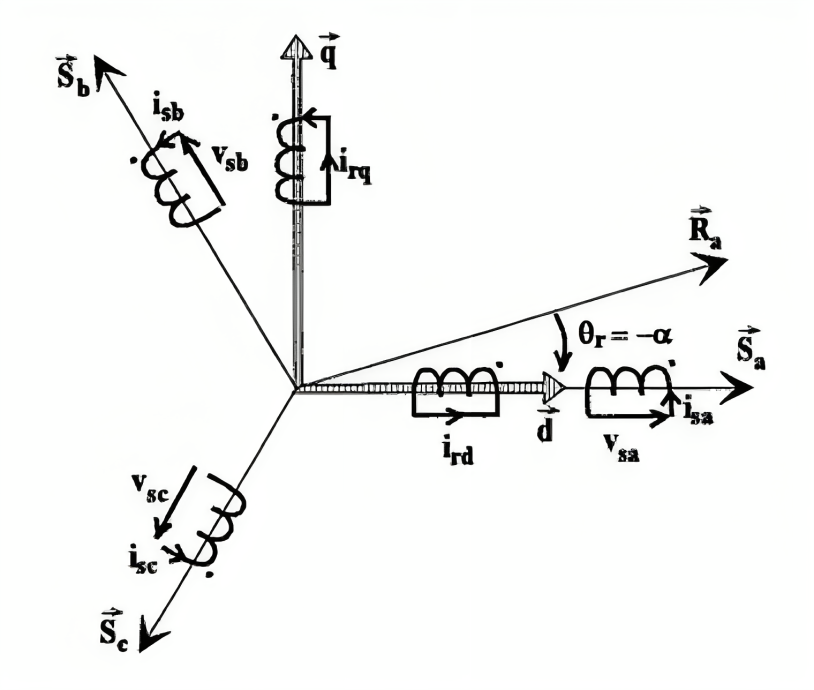
\includegraphics[width=0.4\textwidth]{book_imgs/abc_dq.png} 
    \caption{Transformation du système abc au système dq.}
    \label{img-abc_dq}
\end{figure}

\begin{align}
    \begin{bmatrix}
        v_{\alpha \beta} 
    \end{bmatrix} = 
    \begin{bmatrix}
        T_{23}
    \end{bmatrix} \cdot 
    \begin{bmatrix}
        v_{abc}
    \end{bmatrix} \; ; \;\;\;
    \begin{bmatrix}
        T_{23}
    \end{bmatrix} = \sqrt{\frac{2}{3}}
    \begin{bmatrix}
        1 & \frac{-1}{2} & \frac{-1}{2} \\
        0 & \frac{\sqrt{3}}{2} & \frac{-\sqrt{3}}{2}
    \end{bmatrix}
    \label{eq:T23}
\end{align}

    
Inverse de Concordia $\left[ v_{abc} \right] = [T_{32}] \cdot \left[ v_{\alpha \beta}\right]$  :

\begin{align}
    \begin{bmatrix}
        v_a \\
        v_b \\
        v_c 
    \end{bmatrix} 
    &= 
    \sqrt{\frac{2}{3}}
    \begin{bmatrix}
        1 & 0 \\
        \frac{-1}{2} & \frac{\sqrt{3}}{2} \\
        \frac{-1}{2} & \frac{-\sqrt{3}}{2}
    \end{bmatrix} \cdot 
    \begin{bmatrix}
        v_{\alpha} \\
        v_{\beta} 
    \end{bmatrix}
    \label{eq:T32}
\end{align}

On peut observer dans la relation (\ref{eq:T32}) que $T_{32} = {T_{23}}^{-1} = {T_{23}}^{T}$ \cite{Chattopadhyay2008}, une caractéristique intéressant de la matrice de transformation de Concordia. 

%*******
\FloatBarrier
\subsubsection{Transformée de Clarke :}
%*******

Initialement comme proposé par Edith Clarke \cite{Duesterhoeft1951}, la transformée passe d'un repère a,b,c à un repère $\alpha$, $\beta$ et $o$ :


\begin{align} 
    \begin{bmatrix}
    i_{\alpha}(t) \\
    i_{\beta}(t) \\
    i_{o}(t)
    \end{bmatrix}
    = P \cdot i_{abc}(t) = \frac{2}{3}
    \begin{bmatrix}
    1 & -\frac{1}{2} & -\frac{1}{2} \\
    0 & \frac{\sqrt{3}}{2} & -\frac{\sqrt{3}}{2} \\
    \frac{1}{2} & \frac{1}{2} & \frac{1}{2}
    \end{bmatrix} \cdot
    \begin{bmatrix}
    i_a(t) \\
    i_b(t) \\
    i_c(t)
    \end{bmatrix} 
    \label{eq:Clarke} \\
    \begin{bmatrix}
    i_a(t) \\
    i_b(t) \\
    i_c(t)
    \end{bmatrix}
    = P^{-1}\cdot i_{\alpha\beta}(t) = 
    \begin{bmatrix}
    1 & 0 & 1 \\
    -\frac{1}{2} & \frac{\sqrt{3}}{2} & 1 \\
    -\frac{1}{2} & -\frac{\sqrt{3}}{2} & 1
    \end{bmatrix} \cdot
    \begin{bmatrix}
    i_{\alpha}(t) \\
    i_{\beta}(t) \\
    i_0(t)
    \end{bmatrix}
    \label{eq:Clarke_inv}
\end{align}

Dans la transformation, la composante $o$ permet de détecter les déséquilibres entre les phases du système triphasé. Cela est utile pour le diagnostic de problèmes dans les systèmes électriques et pour la conception de stratégies de contrôle qui peuvent compenser ou gérer ces déséquilibres.

Pour un système triphasée équilibré \cite{Tahri2007}, elle sera donnée pour $\left[v_{\alpha \beta} \right] = \left[Cl\right] \cdot \left[v_{abc} \right]$ :

\begin{equation}
    \begin{bmatrix}
        v_\alpha \\
        v_\beta
    \end{bmatrix} = 
    \frac{2}{3} \cdot 
    \begin{bmatrix}
        1 & -\frac{1}{2} & -\frac{1}{2} \\
        0 & \frac{\sqrt{3} }{2} & -\frac{\sqrt{3} }{2} 
    \end{bmatrix} \cdot
    \begin{bmatrix}
        v_a \\
        v_b \\
        v_c
    \end{bmatrix}
\end{equation}

Et l'inverse de la transformée de Clarke $\left[i_{abc} \right] = \left[Cl\right]^{-1} \cdot \left[i_{\alpha \beta} \right]$ :

\begin{equation}
    \begin{bmatrix}
        v_a \\
        v_b \\
        v_c
    \end{bmatrix} = 
    \frac{2}{3} \cdot 
    \begin{bmatrix}
        1 & 0 \\
        -\frac{1}{2} & \frac{\sqrt{3}}{2} \\
        -\frac{1}{2} & -\frac{\sqrt{3}}{2}
    \end{bmatrix} \cdot
    \begin{bmatrix}
        v_\alpha \\
        v_\beta 
    \end{bmatrix}
\end{equation}

Contrairement à la transformation de Concordia qui conserve la puissance du système, la transformation de Clarke conserve l'amplitude des signaux mais pas nécessairement leur puissance.

%*******
\FloatBarrier
\subsubsection{Transformée de Park :}
%*******

La matrice de rotation de Park peut être facilement comprise à partir de l'image \ref{img-dq_alphabeta}, qui montre comme le axe d va être projeté sur le axe $\alpha$ a partir du cosinus de $\theta$ e le axe $\beta$ a partir du sinus de $\theta$. Le même sera fait pour les projections du axe q, qui a sa fois aura une décalage de $+\pi/2$ con relation au axe d. Alors, sa projection sur $\alpha$ sera donnée pour $cos(\theta - \pi/2) = - sin(\theta)$ et sur le axe $\beta$, $sin(\theta - \pi/2) = cos(\theta)$. En fin de compte, nous générerons le relation \ref{eq:dq_alphabeta}. 

\begin{figure}[!h]
    \centering
    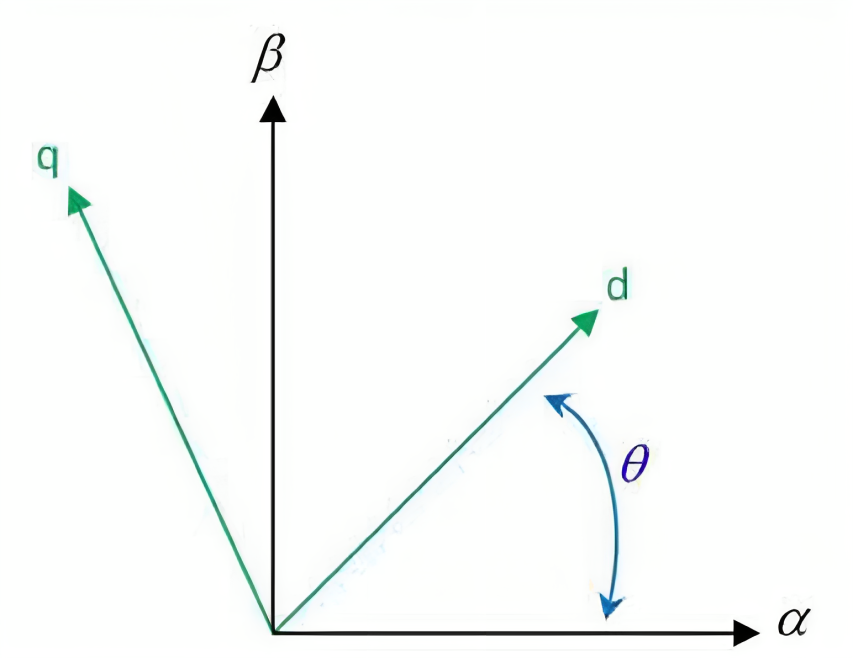
\includegraphics[width=0.4\textwidth]{book_imgs/dq_alphabeta.png} 
    \caption{Rotation du repère $\alpha\beta$ vers le repère dq.}
    \label{img-dq_alphabeta}
\end{figure}

\begin{equation}
    \begin{bmatrix}
        v_d \\
        v_q
    \end{bmatrix} = 
        P(-\theta) \cdot
    \begin{bmatrix}
        v_\alpha \\
        v_\beta 
    \end{bmatrix} \;\; ; \;\;\;
    P(-\theta) =
     \begin{bmatrix}
        cos(\theta) & sin(\theta)  \\
        -sin(\theta) & cos(\theta)  \\
    \end{bmatrix}
    \label{eq:dq_alphabeta}
\end{equation}

Nous pouvons aussi faire la transformée inverse qui sera équivalent à $P(-\theta)^{-1} = P(-\theta)^T = P(\theta)$, où :

\begin{equation}
    \begin{bmatrix}
        v_\alpha \\
        v_\beta 
    \end{bmatrix} = 
        P(\theta) \cdot
    \begin{bmatrix}
        v_d \\
        v_q 
    \end{bmatrix} \;\; ; \;\;\;
    P(\theta) =
     \begin{bmatrix}
        cos(\theta) & -sin(\theta)  \\
        sin(\theta) & cos(\theta)  \\
    \end{bmatrix}
    \label{eq:alphabeta_dq}
\end{equation}

La principale utilité de la transformée de Park est l'expansion des capacités de la transformé de Clarke ou Concordia pour le contrôle des machines tournantes, depuis que, comme elle utilise l'angle $\theta$ dans ça construction, c'est possible qu'elle soit exécuté en continu pendant le contrôle et que $\theta$ soit varié dans la même vitesse de rotation du rotor de la machine. Ainsi, les composantes de courant vont apparaître comme étant continues considérant un glissement de champ nulle. Cela va permettre d'exécuter un contrôle linéaire des courants. 




%==========================================================================
%**************************************************************************
\FloatBarrier
\subsection{La machine asynchrone triphasée à cage}
%**************************************************************************
%==========================================================================

Cette section expose les principes et les équations régissant le fonctionnement et le contrôle vectoriel d'une machine asynchrone triphasée à cage. Elle explique aussi comment le modèle correspondant a été élaboré et implémenté dans Simulink, fournissant un aperçu pratique de sa configuration.

%---------------------------------------
\FloatBarrier
\subsubsection{Équations}
%---------------------------------------

Pour modéliser un moteur asynchrone (modèle à cage, Figure \ref{img-zureks}), il faut d'abord analyser la relation entre les interactions générées entre le rotor et son stator. Dans la pratique, le moteur triphasé aura plusieurs pôles, mais pour des raisons de simplicité, il peut être analysé comme indiqué dans la Figure \ref{img-stator_rotor}, avec un seul pôle triphasé.

\begin{figure}[!h]
    \centering
    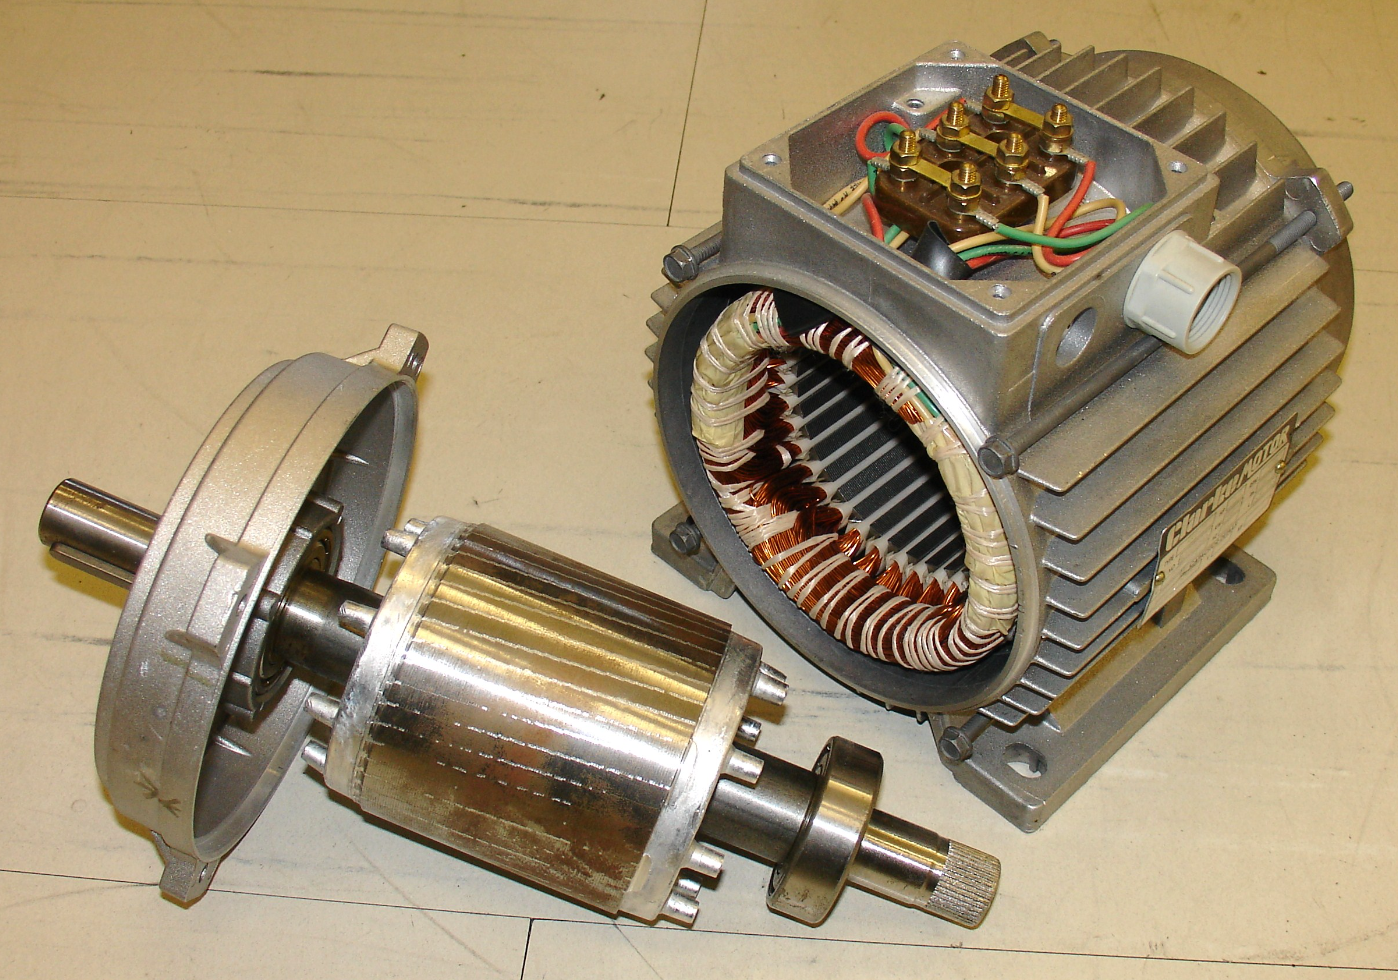
\includegraphics[width=0.6\textwidth]{imgs_pics/zureks.png} 
    \caption{Stator et rotor de moteur asynchrone à cage. \cite{Zureks}}
    \label{img-zureks}
\end{figure}

\begin{figure}[!h]
    \centering
    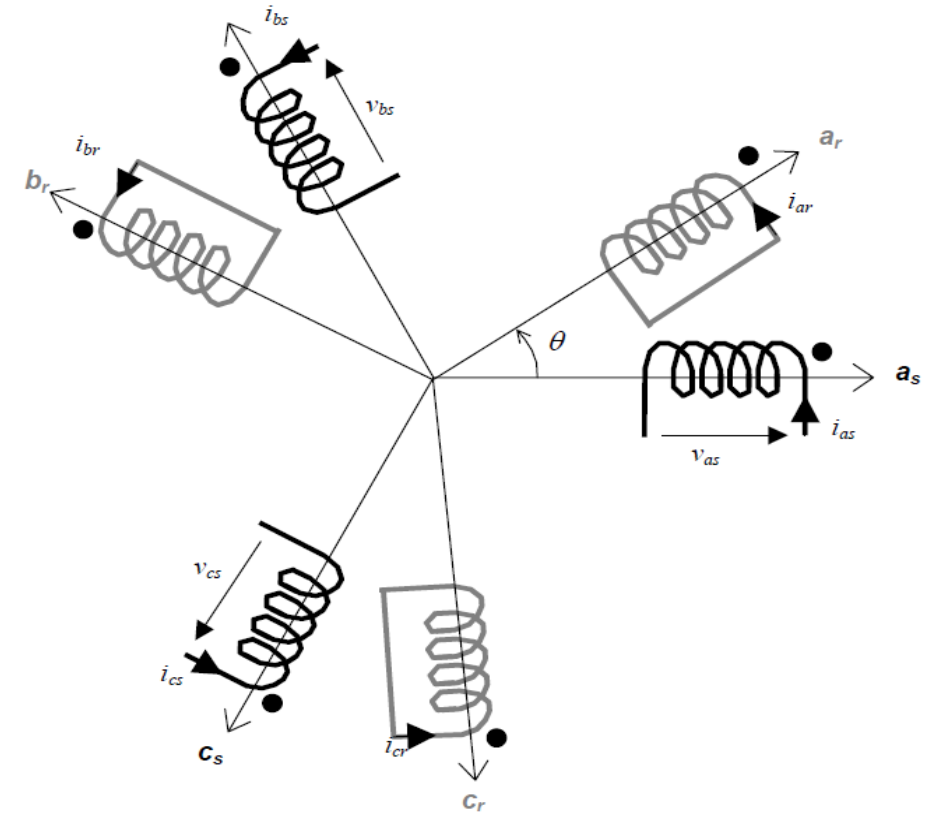
\includegraphics[width=0.4\textwidth]{book_imgs/stator_rotor.png} 
    \caption{Représentation des enroulements statoriques et rotoriques d'une machine asynchrone à rotor bobiné.}
    \label{img-stator_rotor}
\end{figure}

L'équation différentielle décrivant le flux magnétique $\varphi$ dans une bobine (ou inducteur) peut être dérivée de la loi de Faraday pour l'induction électromagnétique. Cette loi stipule que la tension induite dans une bobine est directement proportionnelle à la variation temporelle du flux magnétique à travers la bobine. Ainsi, mathématiquement ça sera exprimée pour $V = -N\frac{d\varphi}{dt}$ où $N$ est le numéro de spires de la bobine. Considérant le modèle des enroulements de l'image \ref{img-stator_rotor} et considérant qu'en plus de l'indutance il aura une résistance (suivant la loi de Ohm), le système des équations des tensions dans le stator de la machine seront données pour \ref{eq:tensions_stator} : 

\begin{equation}
    \left\{
    \begin{align}
        &V_{as}(t) = R_s \cdot i_{as}(t) + \frac{d \varphi_{as}(t)}{dt} \\
        &V_{bs}(t) = R_s \cdot i_{bs}(t) + \frac{d \varphi_{bs}(t)}{dt} \\
        &V_{cs}(t) = R_s \cdot i_{cs}(t) + \frac{d \varphi_{cs}(t)}{dt}
    \end{align} \right.
    \label{eq:tensions_stator}
\end{equation}


Pour présenter un modèle dynamique régissant le comportement d'une machine à induction, les hypothèses suivantes ont été adoptées :

\begin{itemize}
    \item bobinage réparti pour donner une fmm sinusoïdale lorsque le courant est sinusoïdal;
    \item circuit magnétique non-saturé;
    \item phénomènes d’hystérésis, courant de Foucault et effet de peau négligés;
    \item couplages capacitifs des enroulements et phénomènes haute-fréquence négligés;
    \item somme des courants de phases au stator ainsi que celle au rotor est nulle.
\end{itemize}

À partir de la Figure \ref{img-stator_rotor}, se basant sur la relation \ref{eq:tensions_stator} présentée, c'est possible d'écrire les équations simplifiées de tension au stator (\ref{eq:tension_stator}) et rotor (\ref{eq:tension_rotor}). C'est possible de noter que les grandeurs associées au stator portent l'indice s et au rotor, r. 

\begin{equation}
    [v_{sabc}] = R_s \cdot [i_{sabc}] + \frac{d [\varphi_{sabc}]}{dt}
    \label{eq:tension_stator}
\end{equation}

\begin{equation}
    [v_{rabc}] = R_r \cdot [i_{rabc}] + \frac{d [\varphi_{rabc}]}{dt}
    \label{eq:tension_rotor}
\end{equation}

Dans les relations présentés, R est la résistance d'une phase, $i$ le courant de phase et $\varphi$ le flux traversant la phase. Ces fluxes sont définis pour la relation \ref{eq:flux}, où $l_s$ est l'inductrice propre d'une phase statorique, $l_r$ des phases rotoriques, $m_s$ et $m_r$ les inductances mutuelles entre deux phases statoriques et rotoriques respectivement. Savant que $m_{sr}$ est le maximum de l'inductance mutuelle entre une phase statorique et rotorique, il est connu que :

\begin{align*}
    m_1 =& m_{sr} \cdot cos(\theta) \\
    m_2 =& m_{sr} \cdot cos\left( \theta - \frac{2 \cdot \pi}{3} \right) \\
    m_3 =& m_{sr} \cdot cos \left( \theta + \frac{2 \cdot \pi}{3} \right) 
\end{align*}

\begin{equation}
    \left[ \begin{array}{c}
    \varphi_{sa} \\
    \varphi_{sb} \\
    \varphi_{sc} \\
    \vdots \\
    \varphi_{ra} \\
    \varphi_{rb} \\
    \varphi_{rc} \\
    \end{array} \right]
    =
    \left[ \begin{array}{ccccccc}
    l_s & m_s & m_s & \dots & m_1 & m_3 & m_2 \\
    m_s & l_s & m_s & \dots & m_2 & m_1 & m_3 \\
    m_s & m_s & l_s & \dots & m_3 & m_2 & m_1 \\
    \vdots & \vdots & \vdots & \ddots & \vdots & \vdots & \vdots \\
    m_1 & m_2 & m_3 & \dots & l_r & m_r & m_r \\
    m_3 & m_1 & m_2 & \dots & m_r & l_r & m_r \\
    m_2 & m_3 & m_1 & \dots & m_r & m_r & l_r \\
    \end{array} \right] \cdot 
    \left[ \begin{array}{c}
    i_{sa} \\
    i_{sb} \\
    i_{sc} \\
    \vdots \\
    i_{ra} \\
    i_{rb} \\
    i_{rc} \\
    \end{array} \right]
    \label{eq:flux}
\end{equation}

Appliquant la transformée de Concordia à relation des fluxes \ref{eq:flux}, on obtient l'expression suivante :

\begin{equation}
    \begin{bmatrix}
        [\varphi_{s\alpha \beta}] \\
        [\varphi_{r\alpha \beta}]
    \end{bmatrix} = 
    \begin{bmatrix}
        [L_s] & [M(\theta)] \\
        [M(-\theta)] & [L_r]
    \end{bmatrix} \cdot 
    \begin{bmatrix}
        [i_{s \alpha \beta}] \\
        [i_{r \alpha \beta}]
    \end{bmatrix}
    \label{eq:flux_alphabeta}
\end{equation}

Afin de simplifier encore plus la relation obtenue \ref{eq:flux_alphabeta}, on peut adopter un repère de travail $\theta_s = \theta + \theta_r$, sachant que $\theta_s$ est l'angle entre le repère $[\alpha\beta]_s$ et le repère $[dq]$. Le même s'applique eu repère du rotor. La transformation peut être mieux visualisé par la Figure \ref{img-repere}, que démontre les angles à la gauche et le repère résultat à la droite. Ces rotations vont être exécutés dans la simulation par la transformé de Park présenté par la relation \ref{eq:dq_alphabeta}.

\begin{figure}[!h]
    \centering
    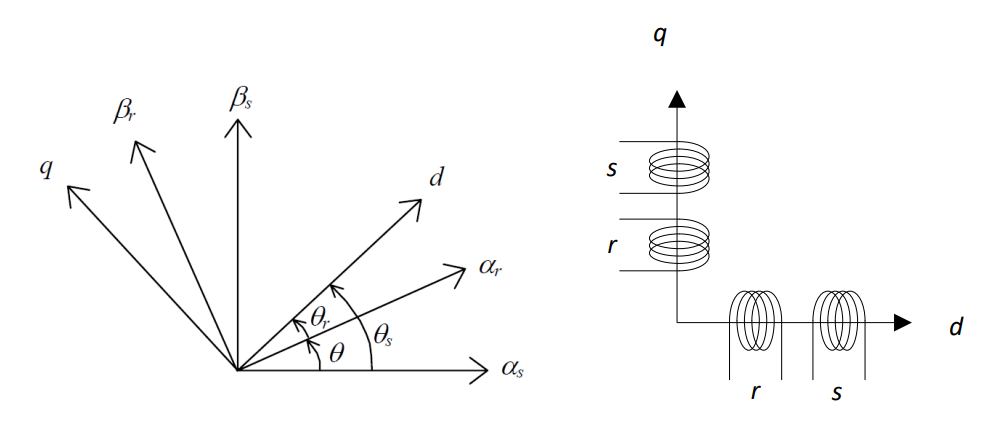
\includegraphics[width=0.8\textwidth]{book_imgs/repere.png} 
    \caption{Repère $\alpha\beta$ statorique, $\alpha\beta$ rotorique et repère dq.}
    \label{img-repere}
\end{figure}

En plus, on aura aussi que $\dot{\theta_s} = \dot{\theta} + \dot{\theta_r}$, depuis que $\omega_s = \omega + \omega_r$. Où chaque $\omega$ représente la vitesse relative du repère $dq$ par rapport au $\alpha\beta$. On aura aussi que $\omega = p \cdot \Omega$, où p est le numéro de pôles de la machine et $\Omega$ la vitesse mécanique du rotor.

A partir des équations \ref{eq:tension_stator} et \ref{eq:flux}, appliquant les transformations de Concordia et Park (\ref{eq:T23}, et \ref{eq:alphabeta_dq}), le modèle suivante est obtenue :


\begin{equation}
    \left\{
    \begin{aligned}
    v_{sd} &= R_s \cdot i_{sd} - \omega_s \cdot \varphi_{sq} + \frac{d\varphi_{sd}}{dt} \\
    v_{sq} &= R_s \cdot i_{sq} + \omega_s \cdot \varphi_{sd} + \frac{d\varphi_{sq}}{dt} \\
    v_{rd} &= R_r \cdot i_{rd} - \omega_r \cdot \varphi_{rq} + \frac{d\varphi_{rd}}{dt} \\
    v_{rq} &= R_r \cdot i_{rq} + \omega_r \cdot \varphi_{rd} + \frac{d\varphi_{rq}}{dt}
    \end{aligned}
    \right.
    \label{eq:tensions_finales}
\end{equation}

\begin{equation}
    \left\{
    \begin{aligned}
    \varphi_{sd} &= L_s \cdot i_{sd} + M_{sr} \cdot i_{rd} \\
    \varphi_{sq} &= L_s \cdot i_{sq} + M_{sr} \cdot i_{rq} \\
    \varphi_{rd} &= L_r \cdot i_{rd} + M_{sr} \cdot i_{sd} \\
    \varphi_{rq} &= L_r \cdot i_{rq} + M_{sr} \cdot i_{sq}
    \end{aligned}
    \right.
    \label{eq:flux_finales}
\end{equation}

Où les fluxes (\ref{eq:flux_finales}) s'appliquent dans l'équation \ref{eq:tensions_finales}, avec $L_s = l_s - m_s$, $L_r = l_r - m_r$ et $M_{sr} = \frac{3}{2} m_{sr}$. Pour une machine asynchrone de alimentation triphasée, nous aurons que $v_{rd} = v_{rq} = 0$.

Par fin, l´équation du couple du moteur est exprimée par :

\begin{equation}
    C_e = p\frac{M_{sr}}{L_r} \cdot (\varphi_{rd} \cdot i_{sq} - \varphi_{rq} - i_{sd})
    \label{eq:Ce-finales}
\end{equation}


%---------------------------------------
\FloatBarrier
\subsubsection{Contrôle vectoriel}
%---------------------------------------


Pour le contrôle de la machine asynchrone triphasée il est possible d'imposer arbitrairement le flux rotorique sur l'axe d, ce qu'il va baser son contrôle vectoriel comme d'une machine synchrone \cite{TPBoileau}. De cette façon, le flux sera concentrée entièrement sur l'axe q, comme montre le système \ref{eq:cont-1-flux} :

\begin{equation}
    \left\{
    \begin{aligned}
    \varphi_{rd} &= \varphi_r \\
    \varphi_{rq} &= \frac{d \varphi_{rq}}{dt} = 0
    \end{aligned}
    \right.
    \label{eq:cont-1-flux}
\end{equation}

Combinant les expressions \ref{eq:Ce-finales} et \ref{eq:cont-1-flux}, l'expression \ref{eq:cont-2-Ce} est obtenue, ressemblant l'équation de couple d'une machine synchrone, qui était l'objective, depuis que l'idée c'est de simplifier d'expressions pour contrôler la machine asynchrone.

\begin{equation}
    C_e = p \frac{M_{sr}}{L_r} \cdot \varphi_r \cdot i_{sq}
    \label{eq:cont-2-Ce}
\end{equation}

A partir des expressions \ref{eq:tensions_finales} et \ref{eq:cont-1-flux}, l'équation \ref{eq:cont-3-0} est obtenue :

\begin{equation}
    0 = R_r \cdot i_{rd} + \frac{d \varphi_r}{dt}
    \label{eq:cont-3-0}
\end{equation}

Ensuite, en utilisant les expressions \ref{eq:flux_finales} et \ref{eq:cont-3-0}, sont obtenues \ref{eq:cont-4-flux} et \ref{eq:cont-5-Lr}, et a partir de ces deux dernières, c'est possible obtenir l'expression de l'évolution du flux rotorique en fonction du courant statorique d'axe d, dans l'expression \ref{eq:cont-6-taur}.

\begin{equation}
    \varphi_{r} = L_{r} \cdot i_{rd} + M_{sr} \cdot i_{sd}; \;\;\; i_{rd} = \frac{\varphi_r M_{sr} \cdot i_{sd}}{L_r}
    \label{eq:cont-4-flux}
\end{equation}

\begin{equation}
    L_r \cdot_{rq} + M_{sr} \cdot i_{sr} = 0; \;\;\; i_{rq} = -\frac{M_{sr}}{L_r}
    \label{eq:cont-5-Lr}
 \cdot i_{sq}\end{equation}


\begin{equation}
    \tau_r \cdot \frac{d \varphi_r}{dt} + \varphi_r = M_{sr} \cdot i_{sd}
    \label{eq:cont-6-taur}
\end{equation}

Dans \ref{eq:cont-6-taur}, la constante de temps rotorique sera donné pour $\tau_r = \frac{L_r}{R_r}$ et il est évident que en régime permanent le flux rotorique sera uniquement dépendant du courant statorique d'axe d : $\varphi_r = M_{sr} \cdot i_{sd}$. Alors remontant dans l'expression du couple (\ref{eq:cont-2-Ce}), en régime permanent elle sera donnée pour \ref{eq:cont-7-Ce}, qui encore une fois se ressemblera a une expression d'une machine synchrone :


\begin{equation}
    C_e = p \cdot \frac{M_{sr}^2}{L_r} \cdot i_{sd} \cdot i_{sq}
    \label{eq:cont-7-Ce}
\end{equation}

Aussi, en analysant les équations \ref{eq:tensions_finales} et \ref{eq:cont-1-flux}, c'est possible l'obtention de l'expression de la pulsation électrique rotorique (loi d'orientation suivant le flux rotorique) :

\begin{equation}
    \omega_r = \frac{R_r}{L_r} \cdot \frac{M_{sr}}{\varphi_r} \cdot i_{sq}
    \label{eq:cont-8-omegar}
\end{equation}

En considérant que les courants statoriques sont parfaitement régulés en régime permanent électrique ça donnera l'expression suivante :


\begin{equation}
    \omega_r = \frac{1}{\tau_r} \cdot \frac{i_{sqref}}{i_{sdref}}
    \label{eq:cont-9-omegar}
\end{equation}

En remplaçant \ref{eq:cont-1-flux} dans \ref{eq:tensions_finales}, c'est possible d'obtenir le modèle de contrôle de la machine à induction dans le repère dq donné par \ref{eq:cont-10-modele}, où $\frac{di_\phi}{dt} = \frac{i_\phi}{\tau_r} + \frac{i_{sd}}{\tau_r}$, $i_\phi = \frac{\varphi_r}{M_{sr}}$ et $\sigma = 1 - \frac{M_{sr}^2}{L_s \cdot L_r}$. A partir de cette modèle, c'est possible définir les coefficients des contrôleurs PI qui seront appliquées à machine.

\begin{equation}
    \left\{
    \begin{aligned}
    v_{sd} &= \left( R_s + \frac{L_s}{\tau_r} \cdot (1 - \sigma)  \right) \cdot i_{sd} + \sigma\cdot L_{s} \cdot \frac{di_{sd}}{dt} - \sigma \cdot L_s \cdot \omega_s \cdot i_{sq} - \frac{L_s}{\tau_r} \cdot (1- \sigma) \cdot i_{\phi} \\
    v_{sq} &= \left( R_s + \frac{L_s}{\tau_r} \cdot (1 - \sigma) \right) \cdot i_{sq} + \sigma \cdot L_s \frac{di_{sq}}{dt} + \sigma \cdot L_s \cdot \omega_s \cdot i_{sd} + p \cdot \Omega \cdot L_s \cdot (1 - \sigma) \cdot i__{\phi}
    \end{aligned}
    \right.
    \label{eq:cont-10-modele}
\end{equation}

Simplifiant l'expression \ref{eq:cont-10-modele}, considérant quelques termes comme des perturbations négligeables dans le système, c'est possible d'obtenir l'expression \ref{eq:cont-11-modele}, qui simplifiera encore plus le calcul des coefficients du contrôleur.

\begin{equation}
    \left\{
    \begin{aligned}
    v_{sd} &= \left( R_s + \frac{L_s}{\tau_r} \cdot (1 - \sigma)  \right) \cdot i_{sd} + \sigma\cdot L_{s} \cdot \frac{di_{sd}}{dt}  \\
    v_{sq} &= \left( R_s + \frac{L_s}{\tau_r} \cdot (1 - \sigma) \right) \cdot i_{sq} + \sigma \cdot L_s \frac{di_{sq}}{dt} 
    \end{aligned}
    \right.
    \label{eq:cont-11-modele}
\end{equation}

%----------------


\begin{equation}
    dWm = \frac{1}{J} \cdot (C_e - T_{load})
    \label{eq:dWm}
\end{equation}


%---------------------------------------
\newpage
\FloatBarrier
\subsubsection{Modélisation}
%---------------------------------------


Pour la modélisation de la machine asynchrone, la version R2020a de MATLAB/Simulink a été employée. Initialement, une modélisation de base de la machine sans système de contrôle a été réalisée et testée pour validation. Puis, le développement s'est poursuivi avec la conception et l'intégration d'un contrôleur de courant, suivi de l'implémentation d'un contrôleur de tension. Le schéma complet de la simulation pour la machine asynchrone à cage est illustré dans la Figure \ref{img-diagMAS}. De plus, la Figure \ref{img-MAS} détaille la mise en œuvre des transformations et les connexions réalisées pour représenter fidèlement le système.

\begin{figure}[!h]
    \centering
    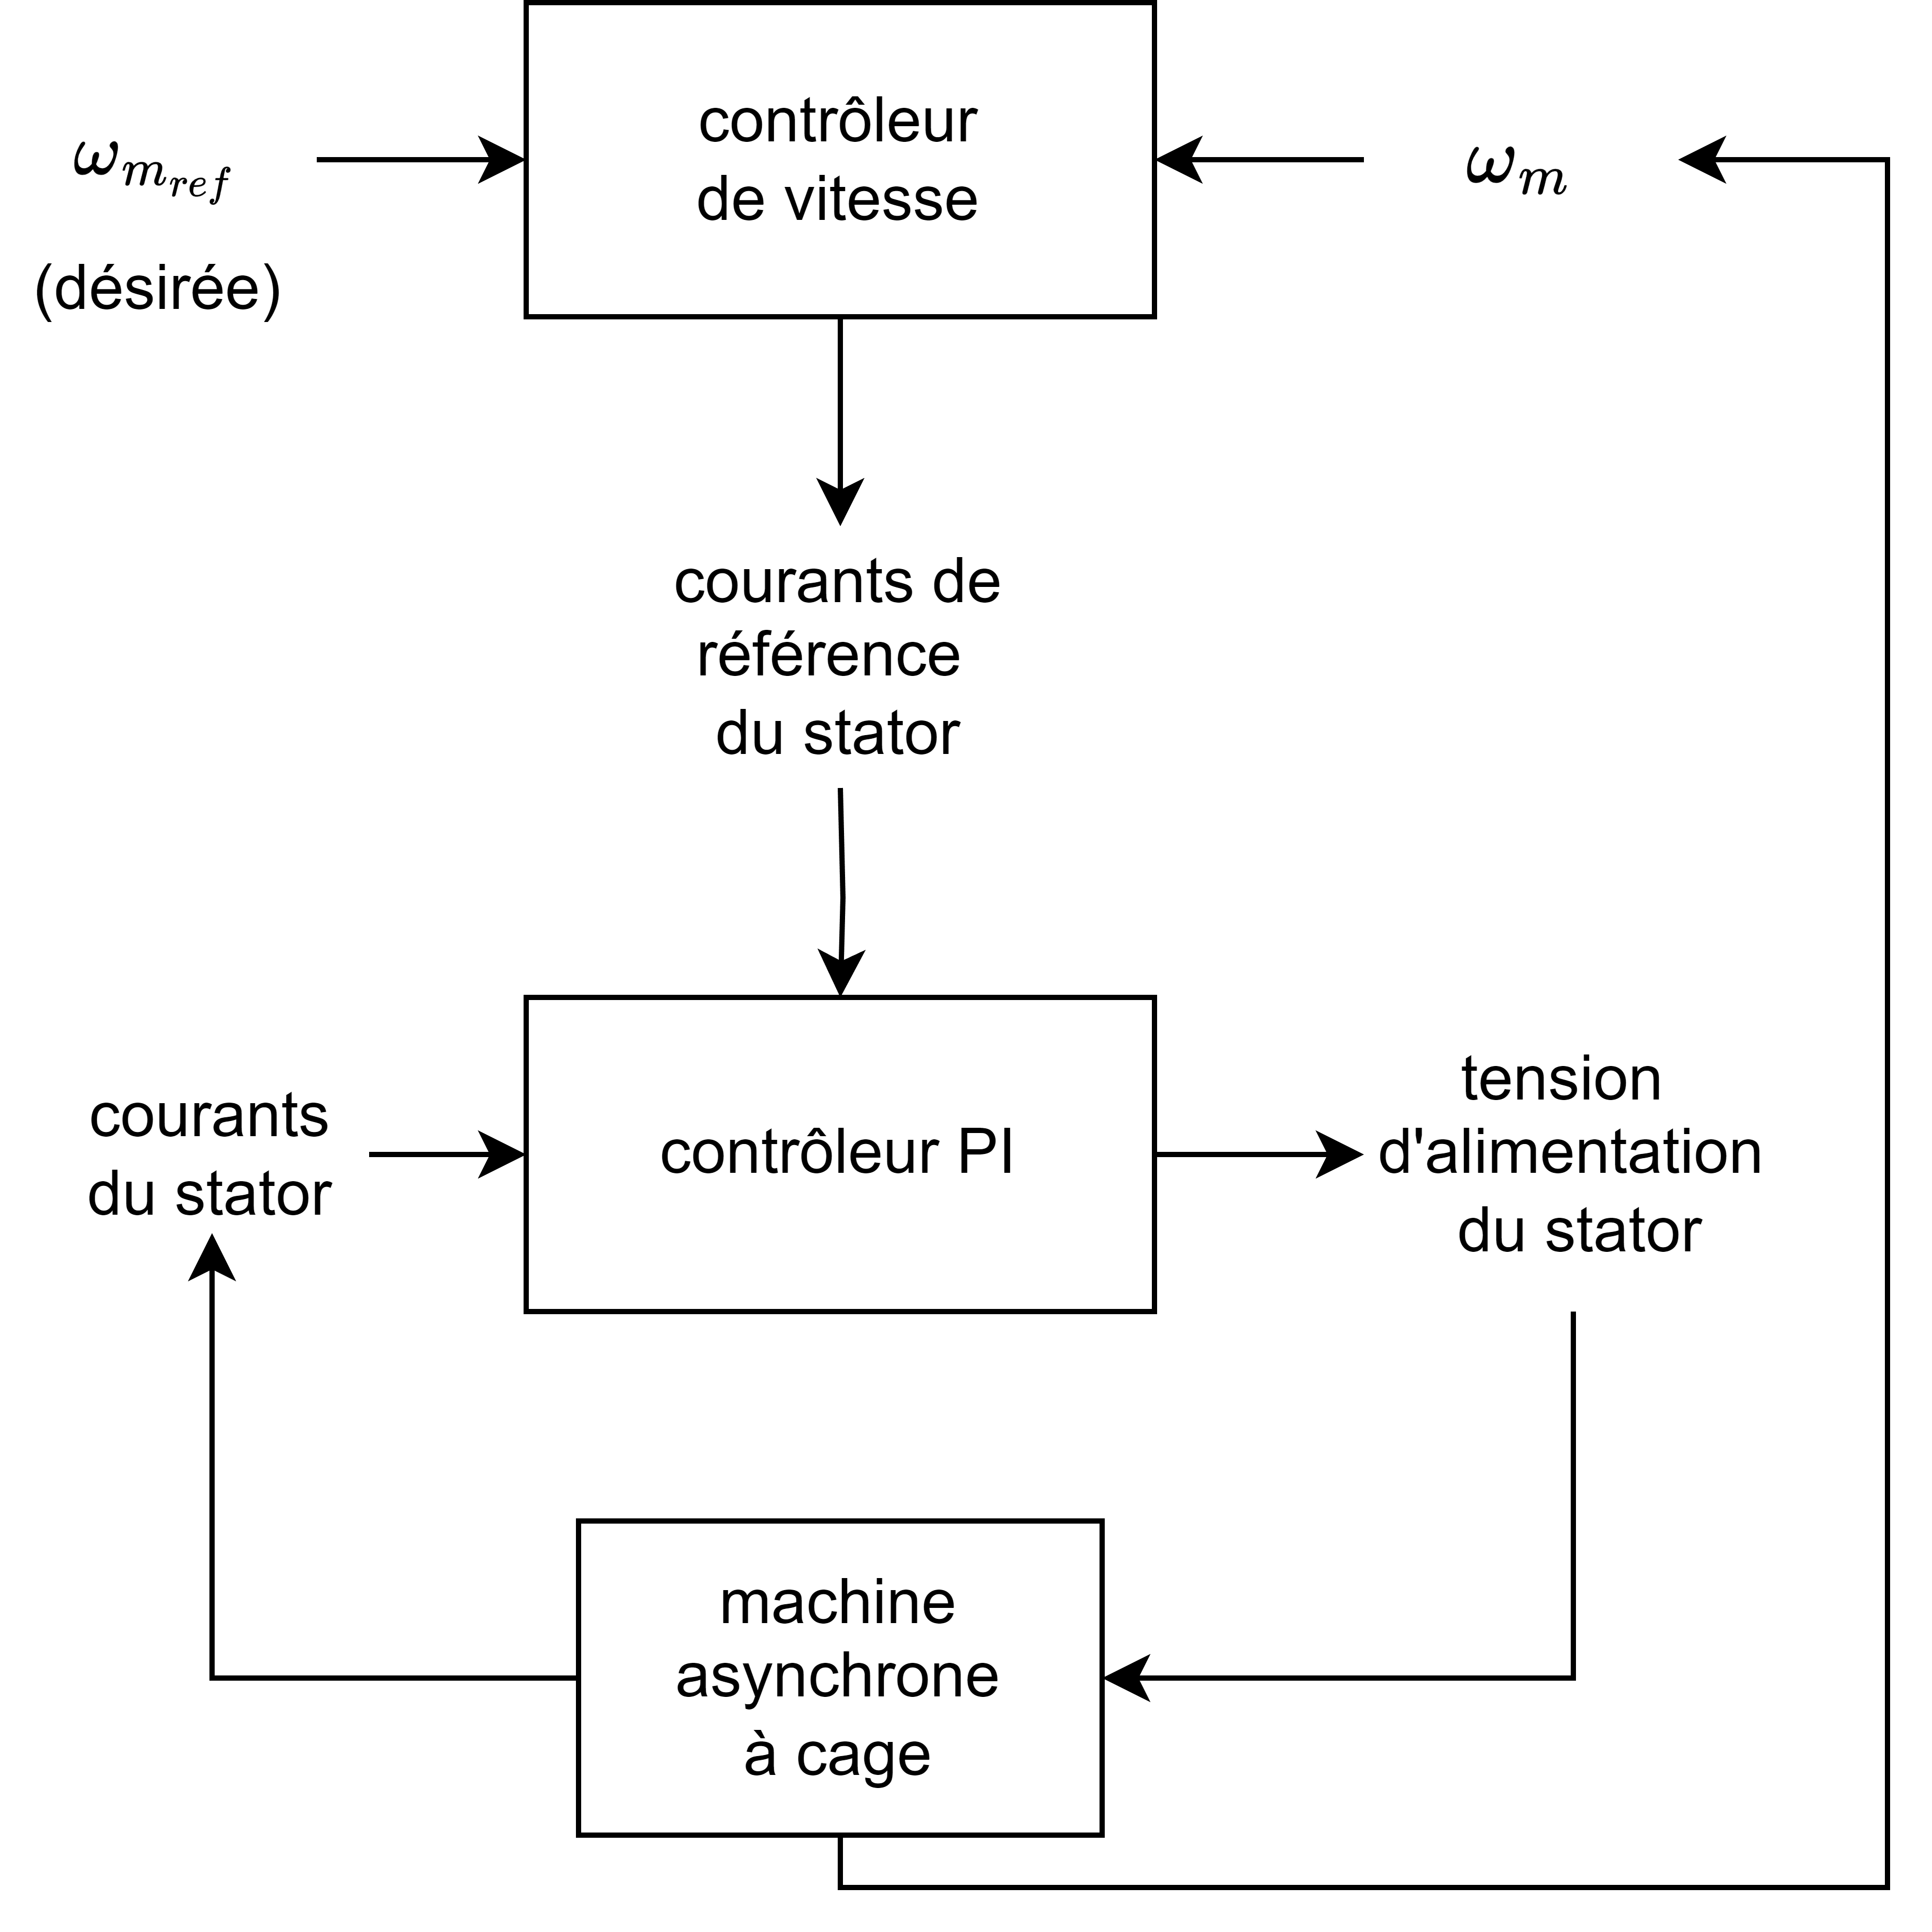
\includegraphics[width=0.6\textwidth]{diagrammes/diagMAS.png} 
    \caption{Schéma de la machine asynchrone à cage et de ses contrôleurs.}
    \label{img-diagMAS}
\end{figure}

La Figure \ref{img-MAS} illustre l'application des transformations de Park et de Concordia, via les équations \ref{eq:T23} et \ref{eq:Clarke}, et leurs inverses (\ref{eq:T32} et \ref{eq:Clarke_inv}), pour le contrôle d'un moteur asynchrone triphasé, représenté par le bloc MAS. Ce moteur, alimenté en tension triphasée $v_{abc}$ au stator, produit des courants triphasés $i_{abc}$ exploités dans une boucle de contrôle fermée. Le rotor, étant court-circuité, n'intervient pas dans l'alimentation électrique. Les courants du stator, une fois transformés dans le repère dq via les transformations de Concordia-Park, permettent de réguler la machine en ajustant la tension d'alimentation en réponse à l'erreur entre les courants mesurés et ceux souhaités. Cette régulation est assurée par un contrôleur de courant, décrit ultérieurement.

\begin{figure}[!h]
    \centering
    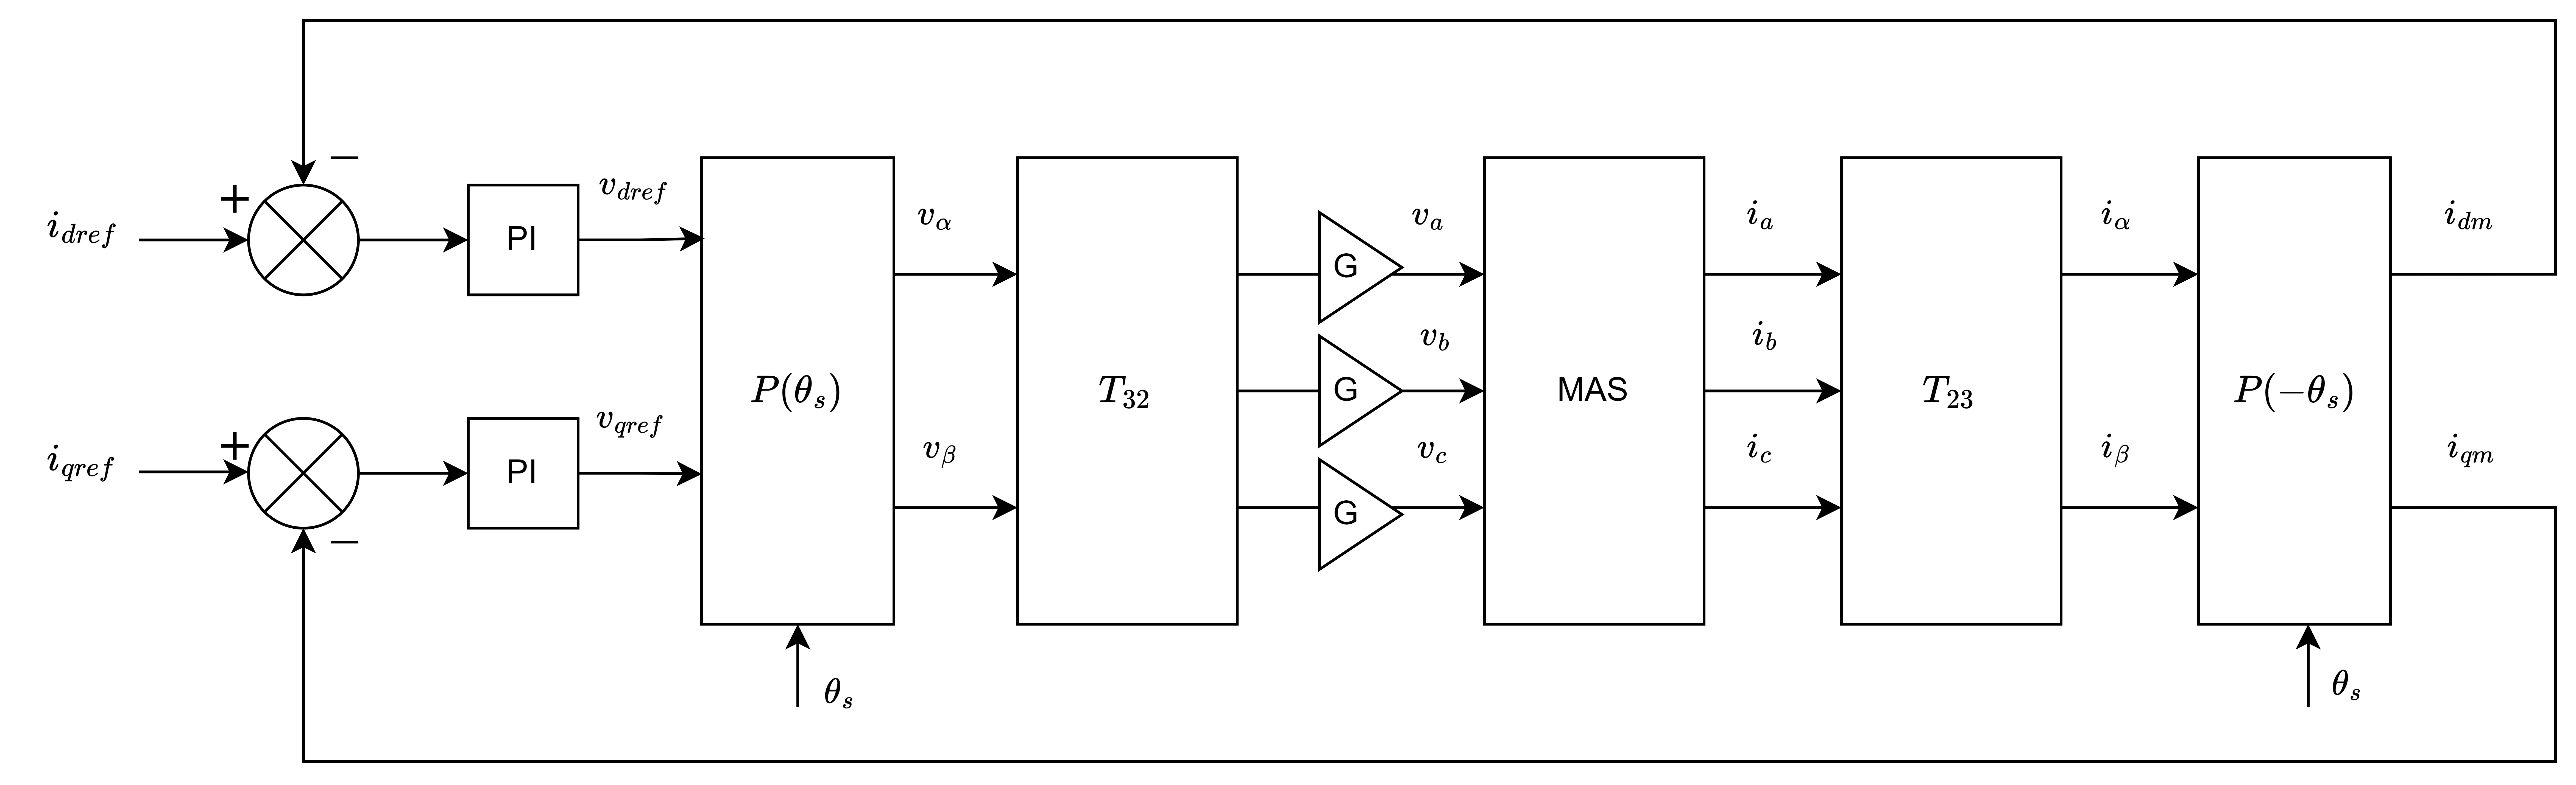
\includegraphics[width=1.0\textwidth]{diagrammes/MAS.png} 
    \caption{Diagramme de bloc en boucle fermée de la machine asynchrone.}
    \label{img-MAS}
\end{figure}

% ==============================================================
\FloatBarrier
\paragraph{MAS}
% ==============================================================

Au sein de Simulink, la première étape a consisté à élaborer un modèle simulant le fonctionnement d'une machine asynchrone à induction. Ce modèle, illustré par la Figure \ref{img-MAS_modele}, est conçu pour accepter une alimentation triphasée en entrée et émuler le comportement d'un moteur réel, basé sur une série de paramètres configurables définis dans les variables de l'environnement MATLAB.


\begin{figure}[!h]
    \centering
    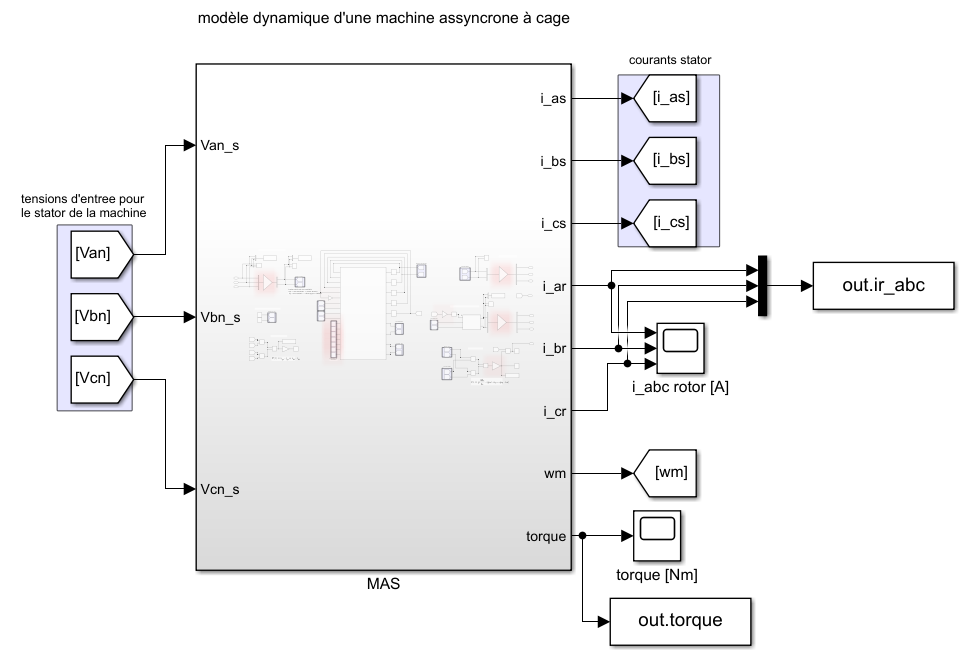
\includegraphics[width=0.8\textwidth]{imgsMATLAB/MAS/MAS/MAS_modele.png} 
    \caption{Sous-système Simulink simulant la machine asynchrone à cage.}
    \label{img-MAS_modele}
\end{figure}

Au cœur de ce sous-système, la fonction MATLAB essentielle simule la dynamique de la machine asynchrone (Figure \ref{img-MASblock_dynamique}). Cette fonction calcule les paramètres de sortie en exécutant une boucle qui intègre les configurations spécifiques de la machine, son alimentation, et résout les équations différentielles clés, illustrées par les références \ref{eq:tension_stator}, \ref{eq:tension_rotor} (notant que, dans un moteur asynchrone, le rotor étant court-circuité, ses tensions sont nulles), \ref{eq:flux_alphabeta}, \ref{eq:cont-2-Ce}, et \ref{eq:dWm}. Cette approche permet de refléter fidèlement le comportement électromécanique de la machine dans la simulation.

\begin{figure}[!h]
    \centering
    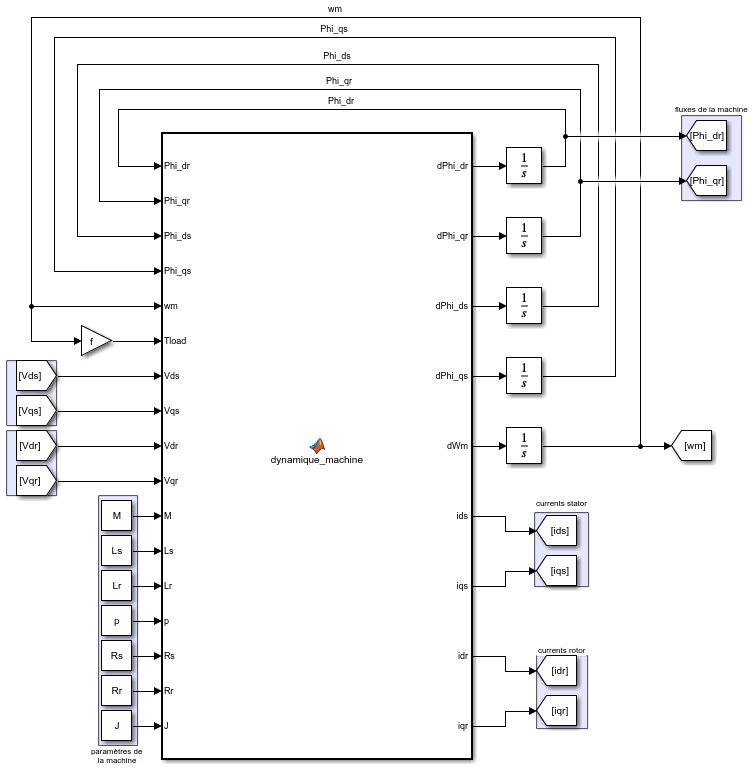
\includegraphics[width=0.8\textwidth]{imgsMATLAB/MAS/MASblock/MASblock_dynamique.png} 
    \caption{Bloc fonctionnel Matlab chargé de simuler la dynamique de la machine asynchrone.}
    \label{img-MASblock_dynamique}
\end{figure}

La figure \ref{img-MASblock_dynamique} montre que la charge appliquée au moteur est générée par le frottement dans la machine et uniquement cela, et qu'aucune charge externe n'a été ajoutée à la simulation. Par conséquent, la charge $T_{load}$ a été calculée en utilisant la relation $T_{load} = \omega_m \cdot f$.

\begin{figure}[!h]
    \centering
    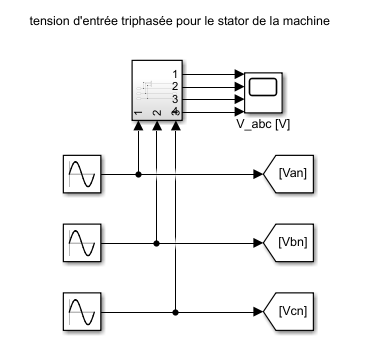
\includegraphics[width=0.5\textwidth]{imgsMATLAB/MAS/MAS/MAS_3f.png} 
    \caption{Alimentation sinusoïdale triphasée. }
    \label{img-MAS_3f}
\end{figure}

Initialement, le stator de la machine a été alimenté avec une tension triphasée pure, illustrée par la Figure \ref{img-MAS_3f}. Puis, dans le sous-système décrit par la Figure \ref{img-MAS_modele}, cette tension a été transposée en repère dq, facilitant ainsi l'analyse et le contrôle, comme expliqué via le schéma de la Figure \ref{img-MASblock/MASblock_tensions}. Cette approche transforme les variables triphasées en composantes directe et quadrature pour simplifier la gestion de la machine.


\begin{figure}[!h]
    \centering
    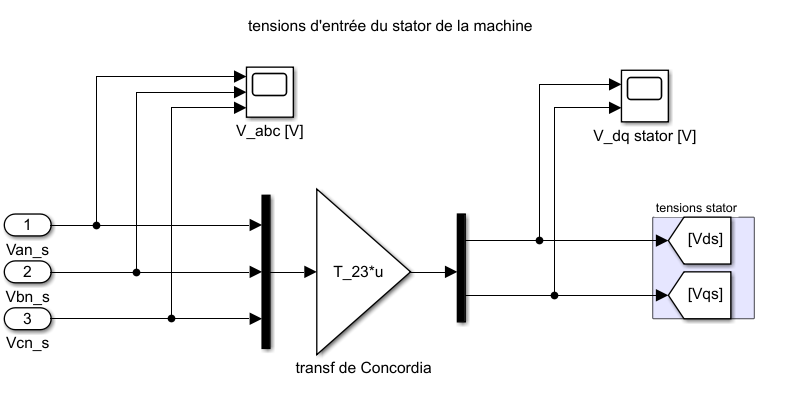
\includegraphics[width=0.8\textwidth]{imgsMATLAB/MAS/MASblock/MASblock_tensions.png} 
    \caption{Application de l'inverse de Concordia (\ref{eq:T23}) pour transformer des tensions biphasés en triphasés.}
    \label{img-MASblock/MASblock_tensions}
\end{figure}


Les transformations de Concordia et Park ont été appliquées aux courants de la machine, permettant une analyse détaillée de son comportement. Dans la Figure \ref{img-MASblock_ir_out}, la transformation de Park est spécifiquement utilisée pour le courant du rotor, facilitant le suivi de son comportement dynamique. Pour déterminer l'angle \(\theta\), il est nécessaire d'intégrer la vitesse de rotation de la machine et d'ajuster cet angle en fonction du nombre de pôles. Concernant les courants du stator, la transformation de Concordia est appliquée, simplifiant l'analyse des courants, comme démontré dans la Figure \ref{img-MASblock_currents_sortie_stator}. Cette méthode permet une représentation simplifiée et précise des paramètres électriques de la machine dans le repère dq.



\begin{figure}[!h]
    \centering
    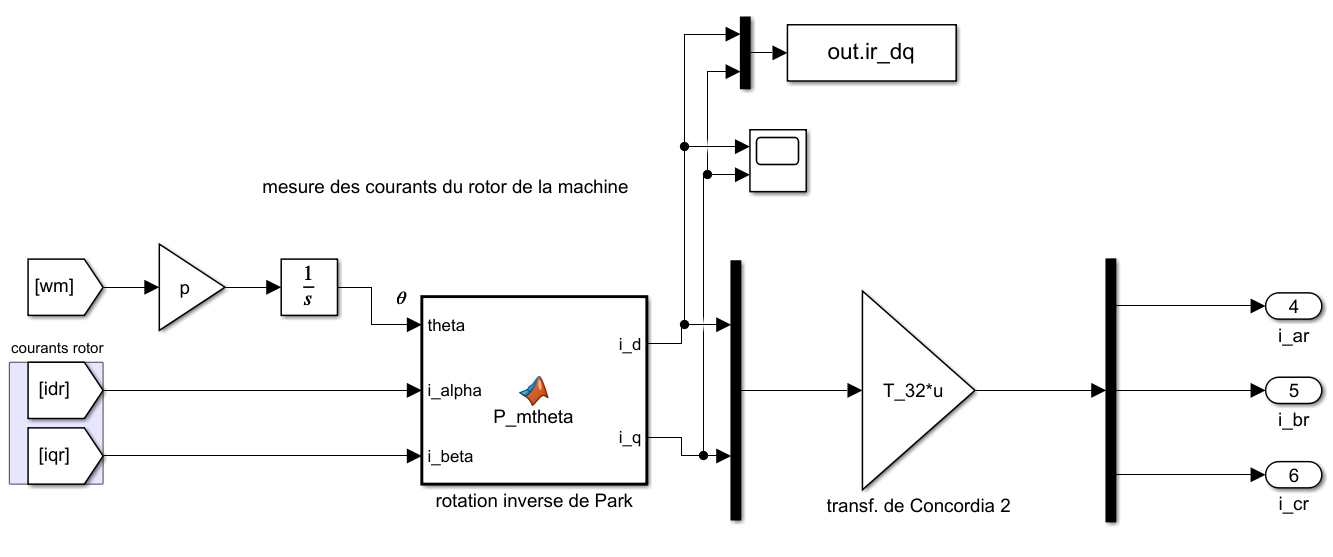
\includegraphics[width=0.9\textwidth]{imgsMATLAB/MAS/MASblock/MASblock_ir_out.png} 
    \caption{Application de l'inverse de Park (\ref{eq:dq_alphabeta}) et Concordia (\ref{eq:T23}) pour obtenir des courants triphasés.}
    \label{img-MASblock_ir_out}
\end{figure}


\begin{figure}[!h]
    \centering
    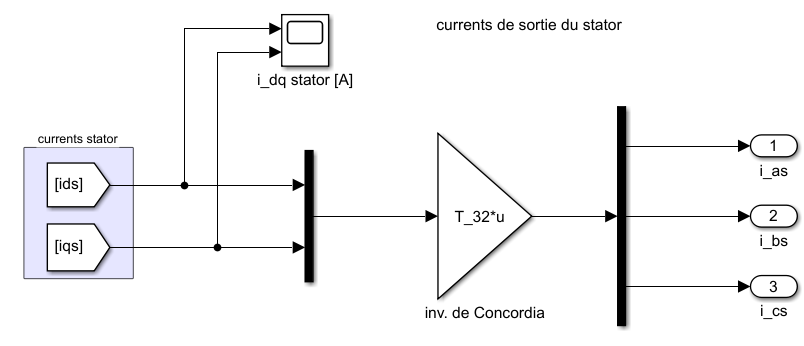
\includegraphics[width=0.8\textwidth]{imgsMATLAB/MAS/MASblock/MASblock_currents_sortie_stator.png} 
    \caption{Application de l'inverse de Concordia (\ref{eq:T32}) pour transformer des courants biphasés en triphasés.}
    \label{img-MASblock_currents_sortie_stator}
\end{figure}



% ==============================================================
\FloatBarrier
\paragraph{Contrôleur de courants}
% ==============================================================

Suite à la modélisation de la machine asynchrone, un contrôleur de courant a été conçu. Ce module évalue l'écart entre les courants statoriques réels et leurs valeurs cibles, ajustant la tension triphasée pour minimiser cette erreur. La Figure \ref{img-diagMAS} met en avant la fonction de ce contrôleur dans le cadre de la simulation, tandis que la Figure \ref{img-MAS_controleur_current} présente le bloc spécifique du contrôleur développé. 

\begin{figure}[!h]
    \centering
    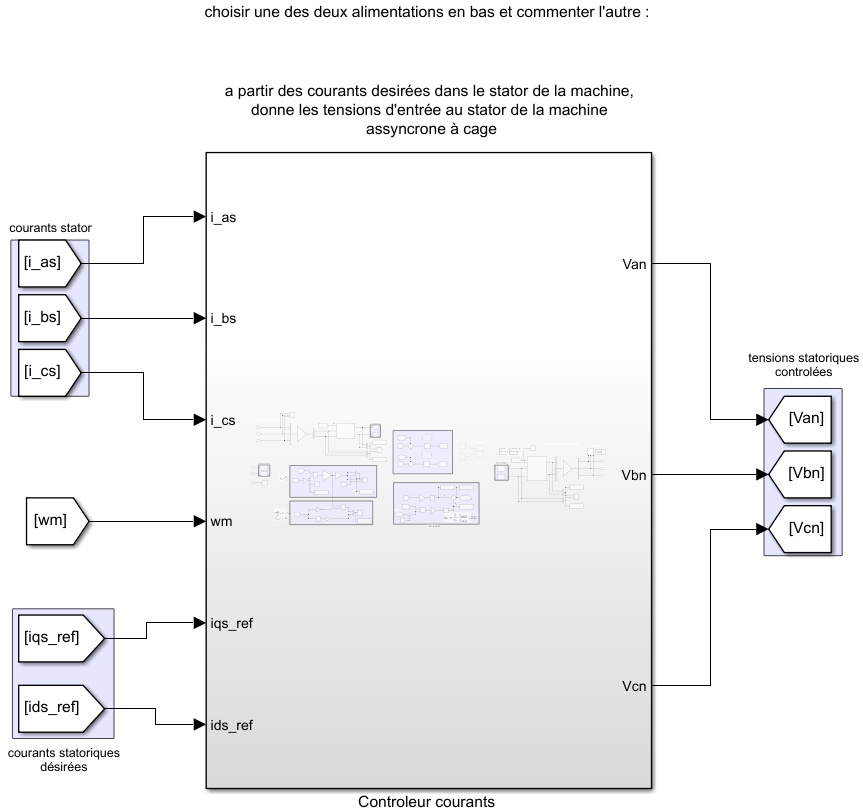
\includegraphics[width=0.9\textwidth]{imgsMATLAB/MAS/MAS/MAS_controleur_current.png} 
    \caption{Bloc fonctionnel Simulink chargé de simuler le comportement du contrôleur de courant de la machine asynchrone.}
    \label{img-MAS_controleur_current}
\end{figure}

Dans le sous-système de contrôle conçu, les courants triphasés du stator sont convertis en repère dq en suivant une méthode semblable à celle employée dans la Figure \ref{img-MASblock_ir_out}. Cette fois, pour traiter les courants statoriques, l'angle $\theta_s$ est utilisé dans la transformation de Park. Basé sur la relation \ref{eq:cont-9-omegar} et considérant que $\theta_s$ est égal à la somme de $\theta_r$ et de $\theta$, comme indiqué dans la Figure \ref{img-repere}, nous parvenons à déterminer l'angle $\theta_s$. La Figure \ref{img-CI_calculThetas} montre comment cet angle est calculé, facilitant ainsi le traitement des courants du stator dans le contexte de contrôle.


\begin{figure}[!h]
    \centering
    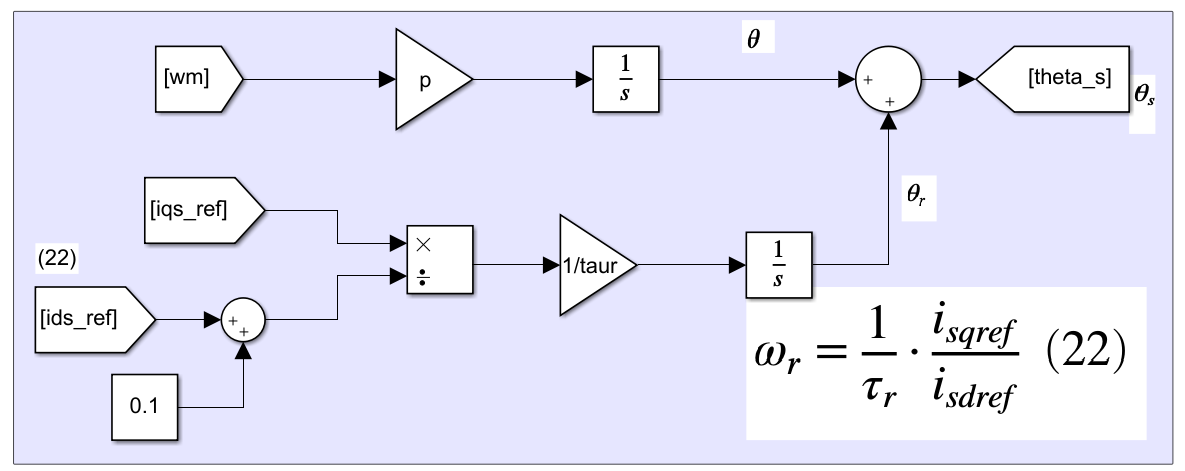
\includegraphics[width=0.7\textwidth]{imgsMATLAB/MAS/CI/CI_calculThetas.png} 
    \caption{Schéma de calcul des angles de phase de la machine asynchrone.}
    \label{img-CI_calculThetas}
\end{figure}

Avec les courants transformés en repère dq, aligné sur l'angle de flux de la machine, le contrôle vectoriel linéaire devient accessible grâce à l'utilisation de régulateurs PI. Simulink offre la fonctionnalité ``Auto tune" pour optimiser les constantes de ces régulateurs, permettant un choix entre une convergence rapide avec moins de robustesse ou une robustesse accrue avec une convergence plus lente. Cette approche est concrétisée dans Simulink, comme le montre la Figure \ref{img-CI_controlePI}.


Pour le calcul manuel des constantes d'un régulateur PI, illustré par le diagramme de la Figure \ref{img-PI}, les constantes \( K_p \) et \( \tau_i \) sont ajustées pour contrôler la réponse du système. La constante \( K_p \) ajuste la réaction immédiate du système à toute erreur instantanée, en amplifiant la commande proportionnelle à l'erreur. En revanche, \( \tau_i \) régule l'action intégratrice, ciblant l'élimination de l'erreur résiduelle sur le long terme et déterminant la vitesse de correction de l'erreur accumulée.


Pour simplifier le calcul des paramètres \( K_p \) et \( \tau_i \), il est utile de séparer le diagramme de la Figure \ref{img-PI} en deux parties distinctes : le modèle de la machine asynchrone et le contrôleur PI lui-même. Cette approche permet d'analyser et d'ajuster séparément la dynamique propre à la machine et la logique de contrôle, facilitant ainsi l'identification des réglages optimaux pour chaque composant. 

\begin{figure}[!h]
    \centering
    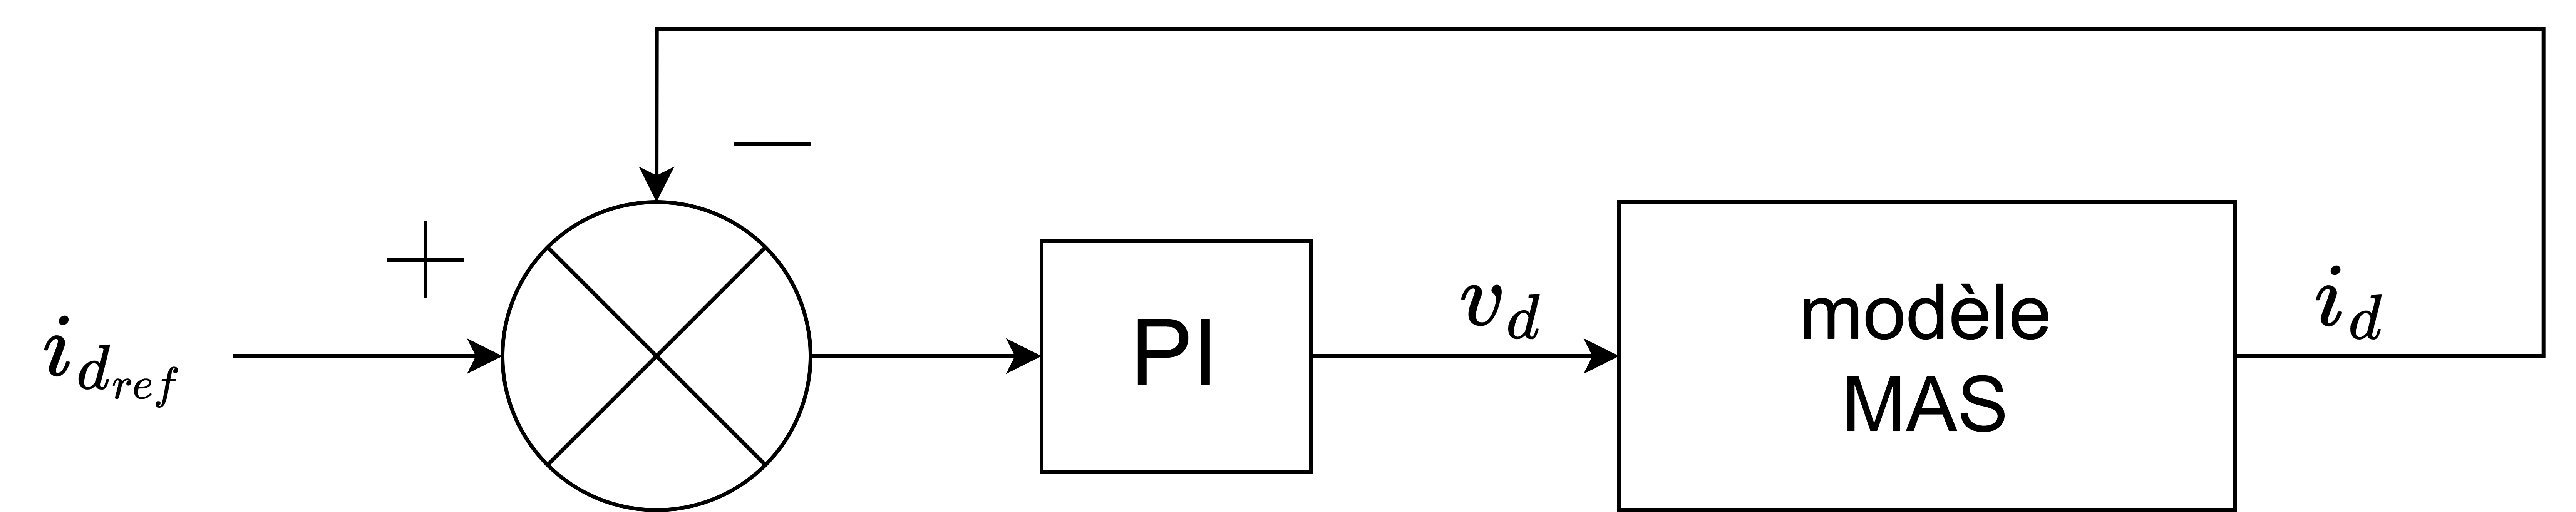
\includegraphics[width=0.8\textwidth]{diagrammes/PI_a.png} 
    \caption{Diagramme du contrôleur PI.}
    \label{img-PI_a}
\end{figure}

\begin{figure}[!h]
    \centering
    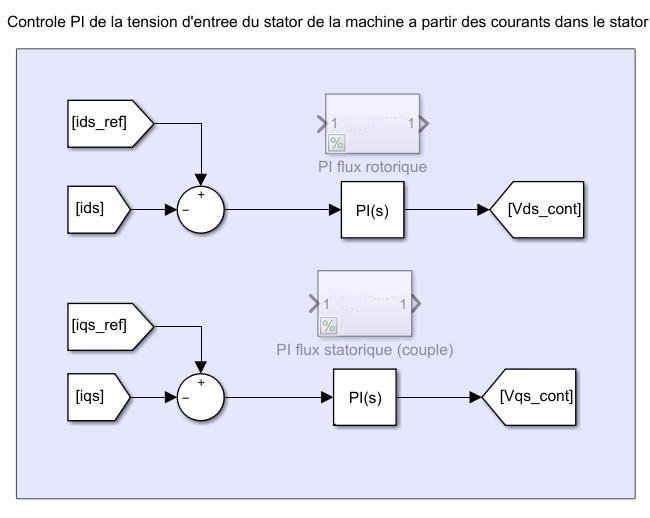
\includegraphics[width=0.6\textwidth]{imgsMATLAB/MAS/CI/CI_controlePI.png} 
    \caption{Diagramme montrant exactement comment les contrôleurs ont été appliqués dans Simulink.}
    \label{img-CI_controlePI}
\end{figure}

\begin{figure}[!h]
    \centering
    
\includegraphics[width=0.9\textwidth]{diagrammes/PI.png} 
    \caption{Diagramme du contrôleur PI.}
    \label{img-PI}
\end{figure}

Comprendre que \( v_d \) est la sortie du contrôleur PI qui influencera directement le stator de la machine nous amène à considérer sa fonction dans le domaine de Laplace comme indiqué par la relation \ref{eq:PI_1}. Pour dériver une fonction de transfert pour la machine asynchrone, le passage par le calcul spécifié dans \ref{eq:PI_2} est nécessaire. Dans cette fonction de transfert, la constante de temps \( \tau_{eq} \), qui est cruciale pour caractériser la réponse temporelle du système, est définie par le rapport \( \frac{L_{eq}}{R_{eq}} \), où \( L_{eq} \) est l'inductance équivalente et \( R_{eq} \) est la résistance équivalente. Cette constante de temps influence directement la vitesse à laquelle le système atteint sa valeur finale après une perturbation, permettant ainsi de définir la rapidité et la réactivité du système face aux changements de commande ou de charge.

\begin{align}
    &v_{d} = \left( R_s + \frac{L_s}{\tau_N} (1 - \sigma) \right) \ccdot i_{d} + \sigma L_s \frac{d i_d}{d\Gamma} \notag \\
    \implies &v_{d} = R_{eq} \cdot i_{d} + L_{eq} \frac{d i_{d}}{d \Gamma} \notag \\
    \implies &V_{d} (s) = R_{eq} \cdot I_{d} (s) + s \cdot L_{eq} \cdot I_{d} (s)
    \label{eq:PI_1}
\end{align}

\begin{equation}
    H_{MAS} (s) = \frac{\text{sortie}}{\text{entrée}} = \frac{I_{d}(s)}{V_{d}(s)} = \frac{1}{R_{eq} + s L_{eq}} = \frac{\frac{1}{R_{eq}}}{1 + s \frac{L_{eq}}{R_{eq}}}
    \label{eq:PI_2}
\end{equation}

\FloatBarrier
Considérant le système en en boucle ouverte :

\begin{align}
    H_{PI} =& K_p \cdot \left( \frac{\frac{1}{R_{eq}}}{1 + s \tau_{eq}} \right) \\
    H_{BO} =& H_{PI} \times H_{MAS} = K_p \left( \frac{1 \tau_i \cdot s}{\tau_i \cdot s} \right) \left( \frac{\frac{1}{R_{eq}}}{1 + s \cdot \tau_{eq}} \right)
\end{align}

Aussi, considérant le système en boucle fermée :

\begin{equation*}
    H_{BF} = \frac{H_{BO}}{1 + H_{BO}}
\end{equation*}

Alors, en prennent $\tau_i = \tau_{eq}$, 

\begin{equation*}
    \implies H_{BF} = \frac{\frac{\frac{1}{R_{eq}} \cdot K_p}{\tau_{eq} \cdot s}}   {1 + \frac{\frac{K_p}{R_{eq}}}{\tau_{eq} \cdot s}} = \frac{1}{1 + \frac{\tau_{eq} \cdot R_{eq}}{K_p}s}
\end{equation*}

Aussi, en faisant $\tau_{BF} = \frac{\tau_{eq}}{3}$ :

\begin{equation*}
    \implies \frac{\tau_{eq} \cdot R_{eq}}{K_p} = \frac{\tau_{eq}}{3}
\end{equation*}

Le $K_p$ sera calculé par $3 \cdot R_{eq}$. C'est ainsi que la boucle fermée illustrée dans la Figure \ref{img-MAS} peut être obtenue. 

% ==============================================================
\FloatBarrier
\paragraph{Contrôleur de vitesse}
% ==============================================================

Pour finaliser le schéma de la Figure \ref{img-diagMAS}, il s'agit maintenant d'intégrer le contrôleur de vitesse, tel que configuré dans Simulink et illustré par la Figure \ref{img-MAS_controleur_vitesse}. Ce contrôleur ajuste le courant de référence \( i_{qs_{ref}} \) en fonction de l'écart entre la vitesse réelle et la vitesse cible de la machine. Le courant de référence \( i_{ds_{ref}} \), indépendant du contrôleur de vitesse, est quant à lui maintenu à 150A.

\begin{figure}[!h]
    \centering
    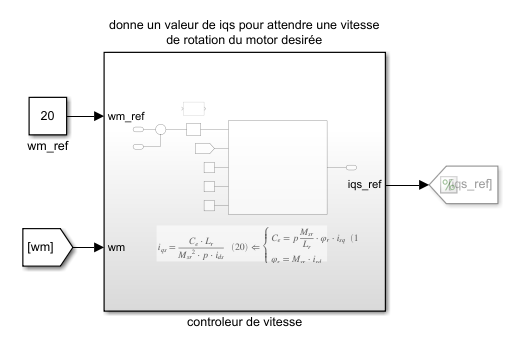
\includegraphics[width=0.8\textwidth]{imgsMATLAB/MAS/MAS/MAS_controleur_vitesse.png} 
    \caption{Bloc fonctionnel Simulink chargé de simuler le comportement du contrôleur de vitesse de la machine asynchrone.}
    \label{img-MAS_controleur_vitesse}
\end{figure}

Le contrôleur dans la Figure \ref{img-MAS_controleur_vitesse} suit le modèle de couplage de la Figure \ref{img-CV_couplage}, en intégrant la relation de couplage \ref{eq:cont-2-Ce}.

\begin{figure}[!h]
    \centering
    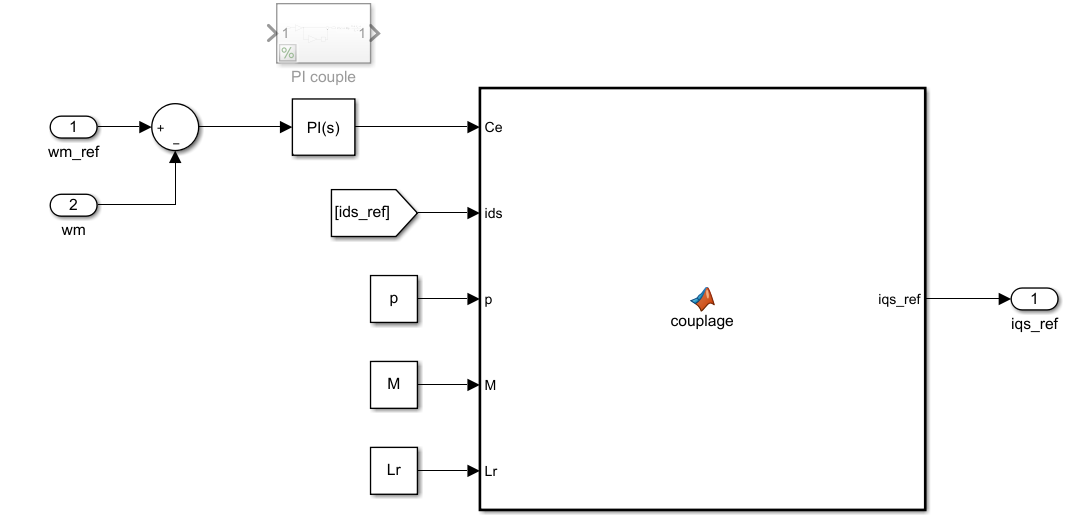
\includegraphics[width=0.8\textwidth]{imgsMATLAB/MAS/CV/CV_couplage.png} 
    \caption{Schéma du contrôleur de vitesse de la machine asynchrone.}
    \label{img-CV_couplage}
\end{figure}







 
%==========================================================================
%**************************************************************************
\FloatBarrier
\subsection{La machine asynchrone à double alimentation}
%**************************************************************************
%==========================================================================

La transition de la modélisation de la machine asynchrone à induction vers celle à double alimentation introduit une capacité de contrôle précis sur le flux magnétique et la vitesse par le biais de deux circuits d'alimentation distincts pour le stator et le rotor. Cette configuration, caractéristique de la machine à double alimentation, permet non seulement l'alimentation traditionnelle du stator mais aussi une alimentation dédiée au rotor. Cette spécificité offre à la machine une flexibilité remarquable pour agir sur le réseau en fournissant soit de la puissance active, soit réactive, par des ajustements fins de l'alimentation rotorique. Dans ce système, le stator est directement connecté au réseau électrique tandis que l'alimentation du rotor est réglée. 

%---------------------------------------
\FloatBarrier
\subsubsection{Équations}
%---------------------------------------

Le modèle de la machine asynchrone à double alimentation (MADA) partage de nombreuses similitudes avec celui de la machine asynchrone à induction décrit précédemment. La distinction majeure réside dans le fait que le rotor de la MADA est alimenté indépendamment, contrairement au rotor en court-circuit de la machine à induction. Ainsi, les équations de modélisation mentionnées pour la machine asynchrone standard sont applicables ici, avec l'équation \ref{eq:tensions_finales}, qui prend en compte \(vr_{dq}\) comme étant non nul.

%---------------------------------------
\FloatBarrier
\subsubsection{Contrôle vectoriel}
%---------------------------------------

La stratégie de commande pour la machine asynchrone à double alimentation reprend les principes appliqués au MAS (Machine Asynchrone Simple). Le dispositif de régulation de courant adopte une approche comparable à celle décrite dans la Figure \ref{img-MAS_controleur_current}. Toutefois, la principale différence réside dans le fait que, pour la machine à double alimentation, c’est le courant du rotor qui est régulé. Ainsi, le régulateur ajuste activement les courants rotoriques, reflétant le contrôle spécifique de l'alimentation du rotor.

Pour réguler les courants dans le rotor de manière analogue, il est nécessaire de transformer ces courants dans le repère dq en utilisant la transformation de Park. Dans ce contexte, l'angle \(\theta_r\) est crucial et se calcule par \(\theta_r = \theta_s - \theta\), où \(\theta_s\) est déterminé à partir de la fréquence du réseau électrique alimentant le stator. Pour le réseau français, par exemple, avec une fréquence de 50 Hz, \(\theta_s\) est obtenu en multipliant cette fréquence par \(2\pi\), ce qui donne la vitesse angulaire. Cette dernière est ensuite intégrée grâce à un bloc intégrateur de Matlab, qui effectue l'opération \(\frac{1}{s}\), pour calculer précisément \(\theta_r\).

Dans le repère dq, pour aligner l'axe d avec le flux statorique \(\varphi_s\), on définit \(\varphi_{ds} = \varphi_s\) et \(\varphi_{qs} = 0\), conformément à \ref{eq:cont-2-Ce}. Avec un réseau électrique fournissant une tension simple \(V_s\) stable, cela résulte en un flux statorique \(\varphi_s\) constant. Cette configuration, en lien avec \ref{eq:cont-2-Ce}, révèle que le couple électromagnétique \(C_{em}\) est directement lié au courant rotorique en quadrature \(i_{qr}\). En outre, en négligeant la résistance des enroulements statoriques, une hypothèse justifiée pour les machines de grande puissance typiquement employées dans la génération d'énergie éolienne (une application courante de la MADA), les expressions des tensions statoriques se simplifient en \ref{eq:MADA1} \cite{Boyette2006}.


\begin{equation}
    \left\{
    \begin{aligned}
        V_{ds} =& \frac{d\varphi_s}{dt} \\
        V_{qs} =& \omega_s \cdot \phi_s
    \end{aligned}
    \right.
    \label{eq:MADA1}
\end{equation}

En savant que $\varphi_{qs} = 0$, c'est possible d'extraire de la relation \ref{eq:flux_finales} :

\begin{equation}
    \left\{
    \begin{aligned}
        \varphi_{ds} = L_s \cdot I_{ds} + M \cdot I_{dr} \\
        0 = L_s \cdot I_{qs} + M \cdot I_{qr}
    \end{aligned}
    \right.
    \label{eq:MADA1_1}
\end{equation}


Avec l'hypothèse du flux statorique constant \ref{eq:MADA2} sera vrai : 

\begin{equation}
    \left\{
    \begin{aligned}
        V_{ds} =& 0 \\
        V_{qs} =& V_s
    \end{aligned}
    \right.
    \label{eq:MADA2}
\end{equation}

À travers de l'équation \ref{eq:MADA1_1}, c'est possible d'établir un lien  entre les courants statoriques et rotoriques :

\begin{equation}
    \left\{
    \begin{aligned}
        I_{ds} =& -\frac{M}{L_s} \cdot I_{dr} + \frac{\phi_s}{L_s} \\
        I_{qs} =& -\frac{M}{L_s} \cdot I_{qs}
    \end{aligned}
    \right.
    \label{eq:MADA3}
\end{equation}

Les puissances actives et réactives peuvent être calculées alors par :

\begin{equation}
    \left\{
    \begin{aligned}
        P =& V_{ds} \cdot I_{ds} + V_{qs} \cdot I_{qs} \\
        Q =& V_{qs} \cdot I_{qs} - V_{ds} \cdot I_{qs}
    \end{aligned}
    \right.
    \label{eq:MADA4}
\end{equation}

Savant que \ref{eq:MADA2} est vrai :


\begin{equation}
    \left\{
    \begin{aligned}
        P =& V_{s} \cdot I_{ds} \\
        Q =& V_{s} \cdot I_{qs} 
    \end{aligned}
    \right.
    \label{eq:MADA5}
\end{equation}

Pour obtenir l'expression des puissances en fonction des courants rotoriques, il faut juste remplacer \ref{eq:MADA3} en \ref{eq:MADA5} :


\begin{equation}
    \left\{
    \begin{aligned}
        P =& - V_{s} \cdot \frac{M}{L_s} \cdot I_{dr} \\
        Q =& - V_{s} \cdot \frac{M}{L_s} \cdot I_{dr} + V_s \frac{\varphi_s}{L_s} 
    \end{aligned}
    \right.
    \label{eq:MADA6}
\end{equation}

A partir des équations \ref{eq:MADA1} et \ref{eq:MADA2}, l'expression suivante pour le flux statorique est obtenue :

\begin{equation}
    \varphi_s = \frac{V_s}{\omega_s}
    \label{eq:MADA7}
 \end{equation}

 Alors à travers de \ref{eq:MADA6} combinée avec \ref{eq:MADA7}, l'expression des puissances peut être simplifiée :

 \begin{equation}
    \left\{
    \begin{aligned}
        P =& - V_{s} \cdot \frac{M}{L_s} \cdot I_{dr}  \\
        Q =& - V_{s} \cdot \frac{M}{L_s} \cdot I_{dr} +  \frac{V_s^2}{L_s \cdot \omega_s} 
    \end{aligned}
    \right.
    \label{eq:MADA8}
\end{equation}

Afin de pouvoir contrôler correctement la machine, c'est nécessaire d'établir la relation entre les courants et les tensions rotoriques qui seront appliqués à la machine. En remplaçant dans l'équation des flux \ref{eq:flux_finales} par l'expression \ref{eq:MADA3}, le système suivante est obtenu :


\begin{equation}
    \left\{
    \begin{aligned}
        \varphi_{dr} =& \left( L_r - \frac{M^2}{L_s} \right) I_{dr} + \frac{M V_s}{L_s \omega_s} \\
        \varphi_{dr} =& \left( L_r - \frac{M^2}{L_s} \right) I_{qr}
    \end{aligned}
    \right.
    \label{eq:MADA9}
\end{equation}

En remplaçant l'expression des flux rotoriques de l'équation précédente \ref{eq:MADA6} par $L_s = l_s - M_s$, $L_r = l_r - M_r$ et $M = \frac{3}{2}M_{sr}$ c'est obtenu :

\begin{equation}
    \left\{
    \begin{aligned}
        V_{dr} =& R_r I_{dr} + \left( L_r  L_s \right)\frac{dI_{dr}}{dt} - g \omega_s (L_r - \frac{M^2}{L_s}) I_{qr} \\
        V_{qr} =& R_r I_{qr} + \left( L_r  L_s \right)\frac{dI_{qr}}{dt} + g \omega_s (L_r - \frac{M^2}{L_s}) I_{dqr} + g 
        \frac{M V_s}{L_s}
        \label{eq:MADA10}
    \end{aligned}
    \right.
    \label{eq:MADA7}
\end{equation}


%---------------------------------------
\FloatBarrier
\subsubsection{Modélisation}
%---------------------------------------

La modélisation de la MADA a suivi celle de la machine asynchrone à induction, en adaptant le modèle de la MAS (Figure \ref{img-MAS_modele}) pour inclure une alimentation active du rotor. Le contrôleur de courant, similaire à celui de la MAS (Figure \ref{img-MAS_controleur_current}), cible désormais les courants rotoriques. L'étape suivante fut de développer un contrôleur de puissance pour la MADA, achevant le schéma de simulation présenté dans la Figure \ref{img-diagMADA} :

\begin{figure}[!h]
    \centering
    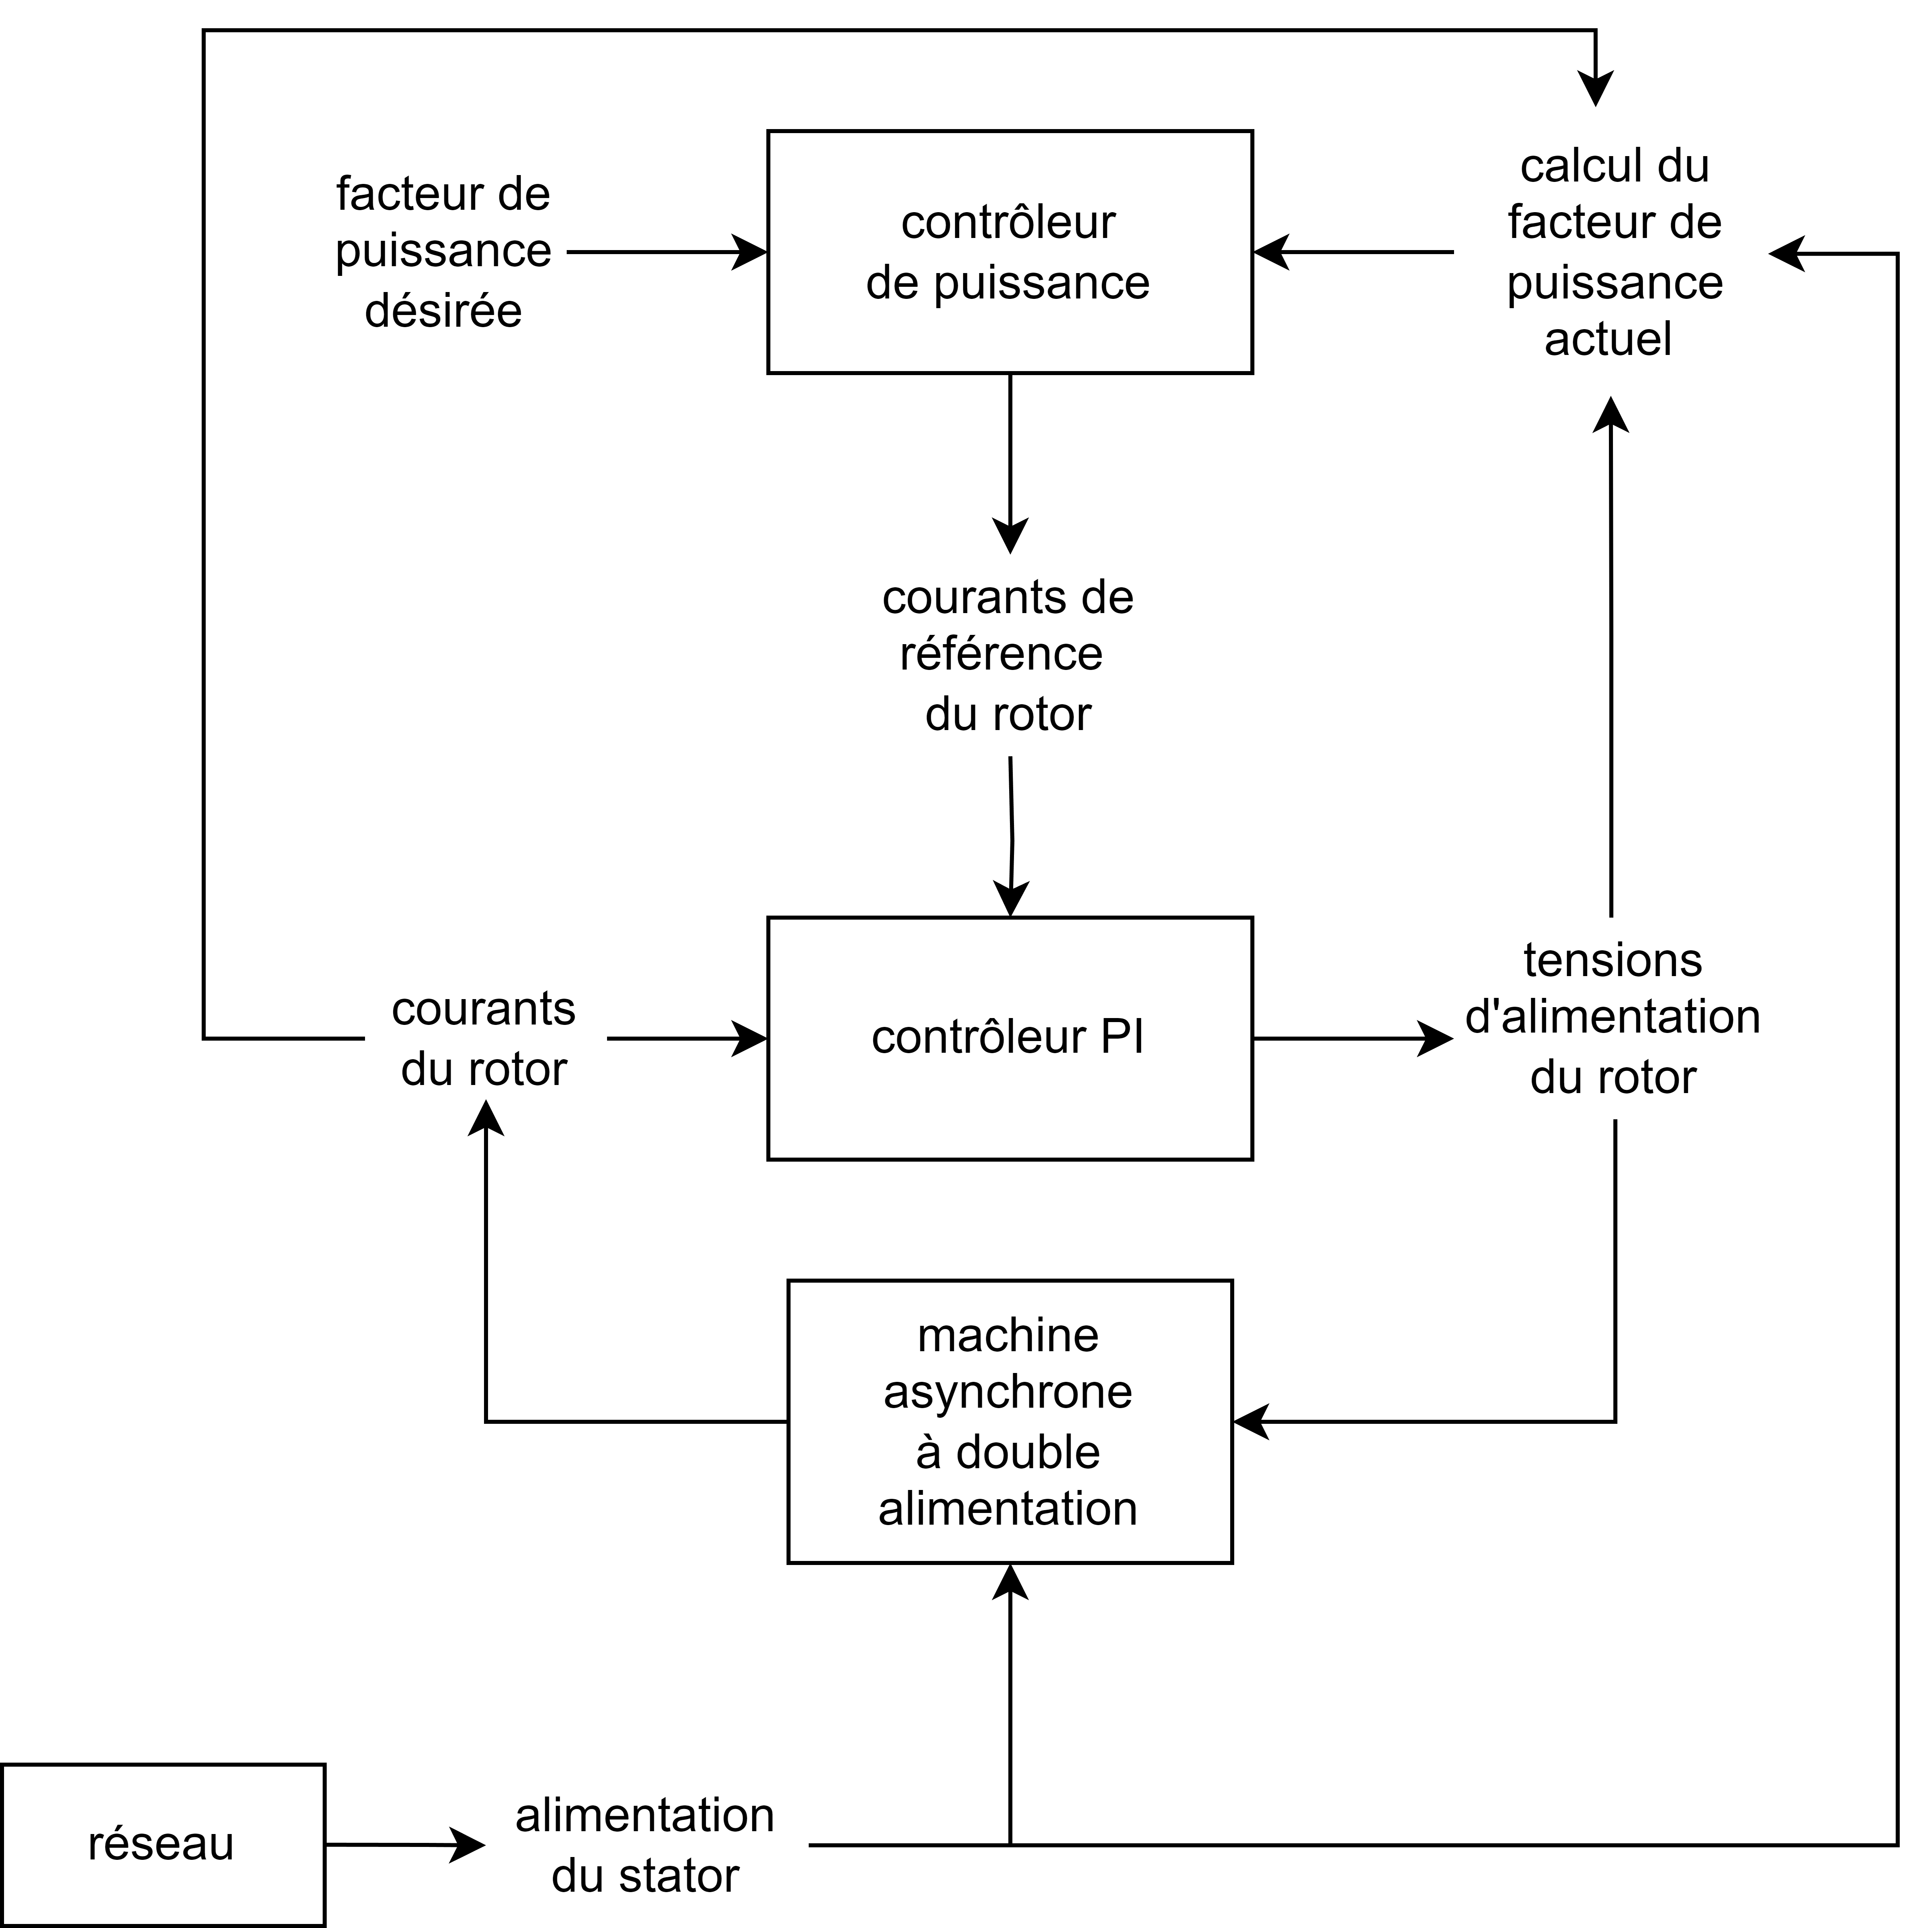
\includegraphics[width=0.7\textwidth]{diagrammes/diagMADA.png} 
    \caption{Schéma de la MADA et ses contrôleurs.}
    \label{img-diagMADA}
\end{figure}

La simulation de la MADA, illustrée dans la Figure \ref{img-MADA}, emploie les transformations de Park et de Concordia pour le changement de repère, similaire à ce qui est présenté pour la MAS dans la Figure \ref{img-MAS}. Le schéma souligne la connexion du réseau au stator et la régulation indépendante de l'alimentation du rotor.


\begin{figure}[!h]
    \centering
    \includegraphics[width=1.0\textwidth]{diagrammes/MADA.png} 
    \caption{Diagramme de bloc en boucle fermée de la MADA.}
    \label{img-MADA}
\end{figure}

Pour le contrôleur de puissance, c'était implémente la relation \ref{eq:MADA8} pour définir les courants $I_{qr}$ et $I_{dr}$ de référence utilisant les valeurs de $P$ et $Q$ désirée en plus des valeurs de $V_{s} = V_{qs}$, $\omega_s$, $M$ et $L_s$.






\newpage
\section{Résultats et discussions}


%---------------------------------------
\subsection{Simulation MAS}
%---------------------------------------


Pour tester la machine virtuelle crée, les paramètres suivantes ont étés adoptées : $p=2; Rs = 3m\Omega; Rr=4.5m\Omega; Ls=210uH; L_r = L_s; M_{sr}=195.5uH; f=1.1 \cdot 10^{-3} kg\cdot m^2 \cdot s^{-1}; J = 10.8 \cdot 10^-3{kg \cdot m^2}$. Aussi, avec ces paramètres et définissant $\tau_i=\tau_{eq}$ et $K_p = 3 \cdot R_{eq}$, c'est possible calculer $\tau_i = 4.1\cdot 10^-3$ et $K_p = 2.07 \cdot 10^-2$.

Dans les simulations, une vitesse cible de \(1500 \frac{rad}{s}\) et des courants de référence de \(150 A\) pour le repère dq du stator ont été établis, isolant ainsi le contrôleur de vitesse pour une analyse plus nette. Cette configuration, choisie pour sa clarté dans l'analyse des données, utilise un intervalle de simulation de 30 secondes avec un simulateur discret à pas fixe de \(10^{-4}\) et un solveur de type Runge-Kutta d'ordre 4.

La courbe de vitesse angulaire du rotor montre une augmentation amortie jusqu'à stabiliser à \(1500 \frac{rad}{s}\), soit \(1.4324 \times 10^4 Hz\). Ce comportement démontre l'efficacité du système à atteindre la vitesse désirée, un aspect positif de la performance de la machine :

% ela poderia ir mais rápido ?

\begin{figure}[!h]
    \centering
    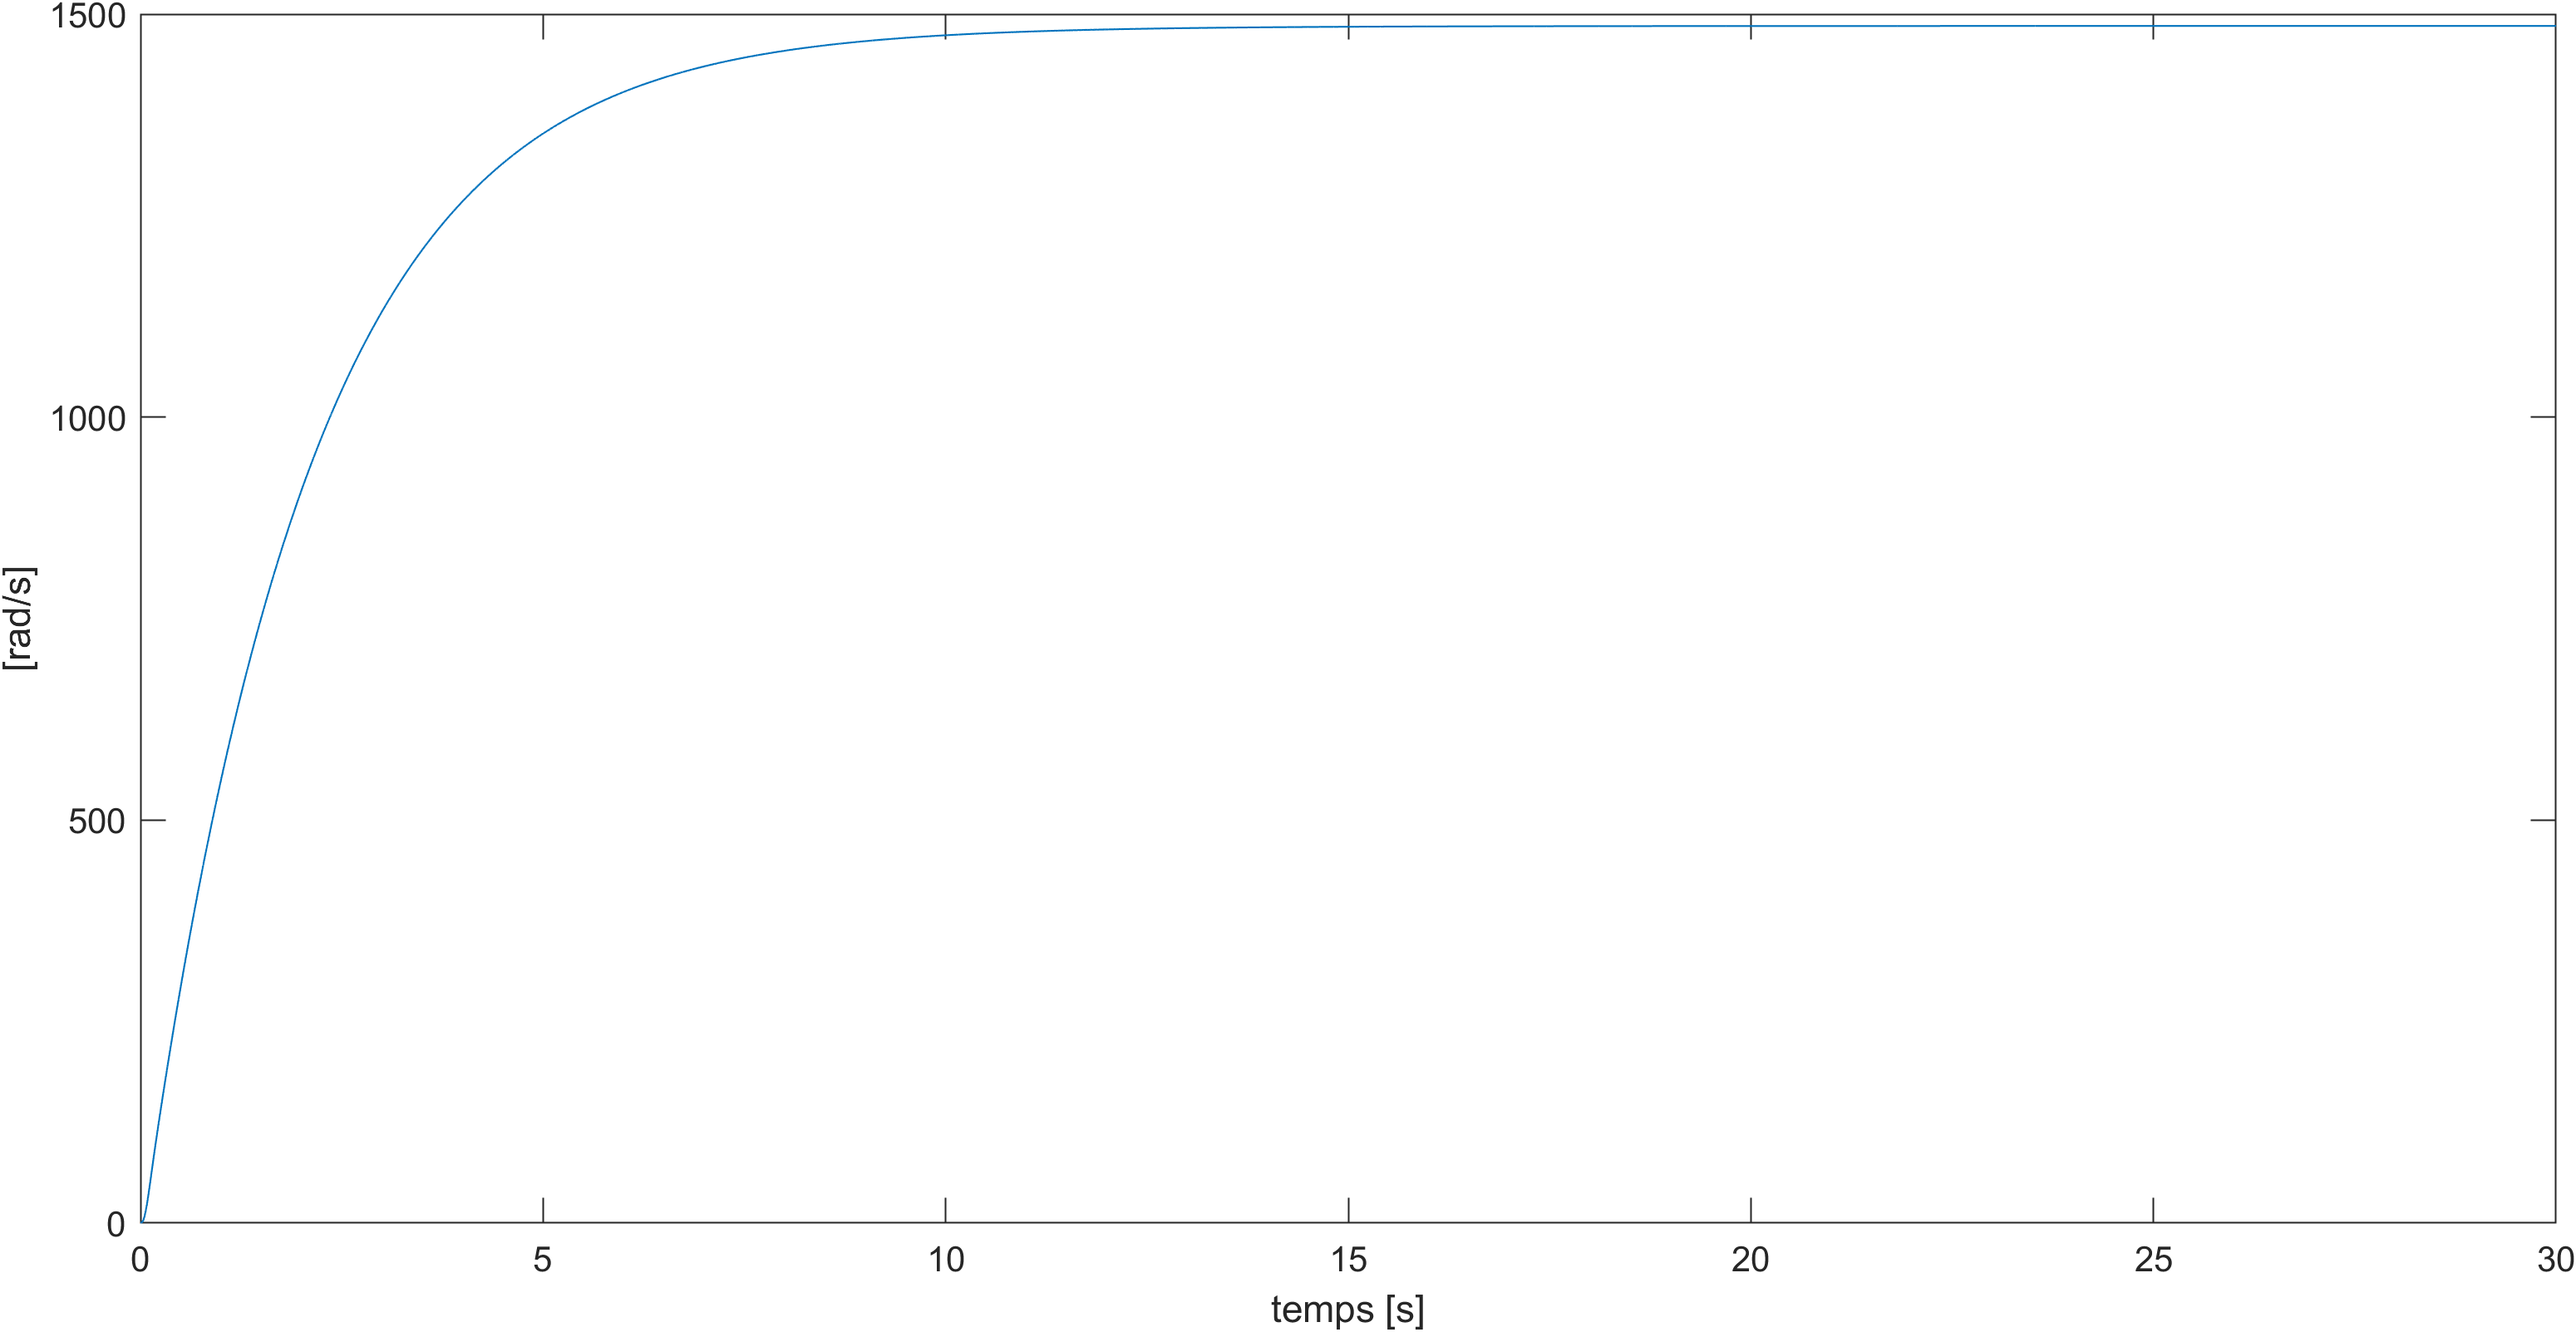
\includegraphics[width=0.8\textwidth]{simusMATLAB/MAS/wm.png} 
    \caption{Vitesse angulaire du rotor de la MAS mesurée au cours du temps.}
    \label{img-simuMatlab-wm}
\end{figure}

La Figure \ref{img-simuMatlab-is_abc} illustrant les courants triphasés dans le stator révèle une phase transitoire dans les premiers dixièmes de seconde, typique d'un démarrage. Passé ce moment, dès 0,2 seconde, les courants alternatifs commencent à converger, indiquant une stabilisation rapide du système sous l'effet du contrôleur.


\begin{figure}[!h]
    \centering
    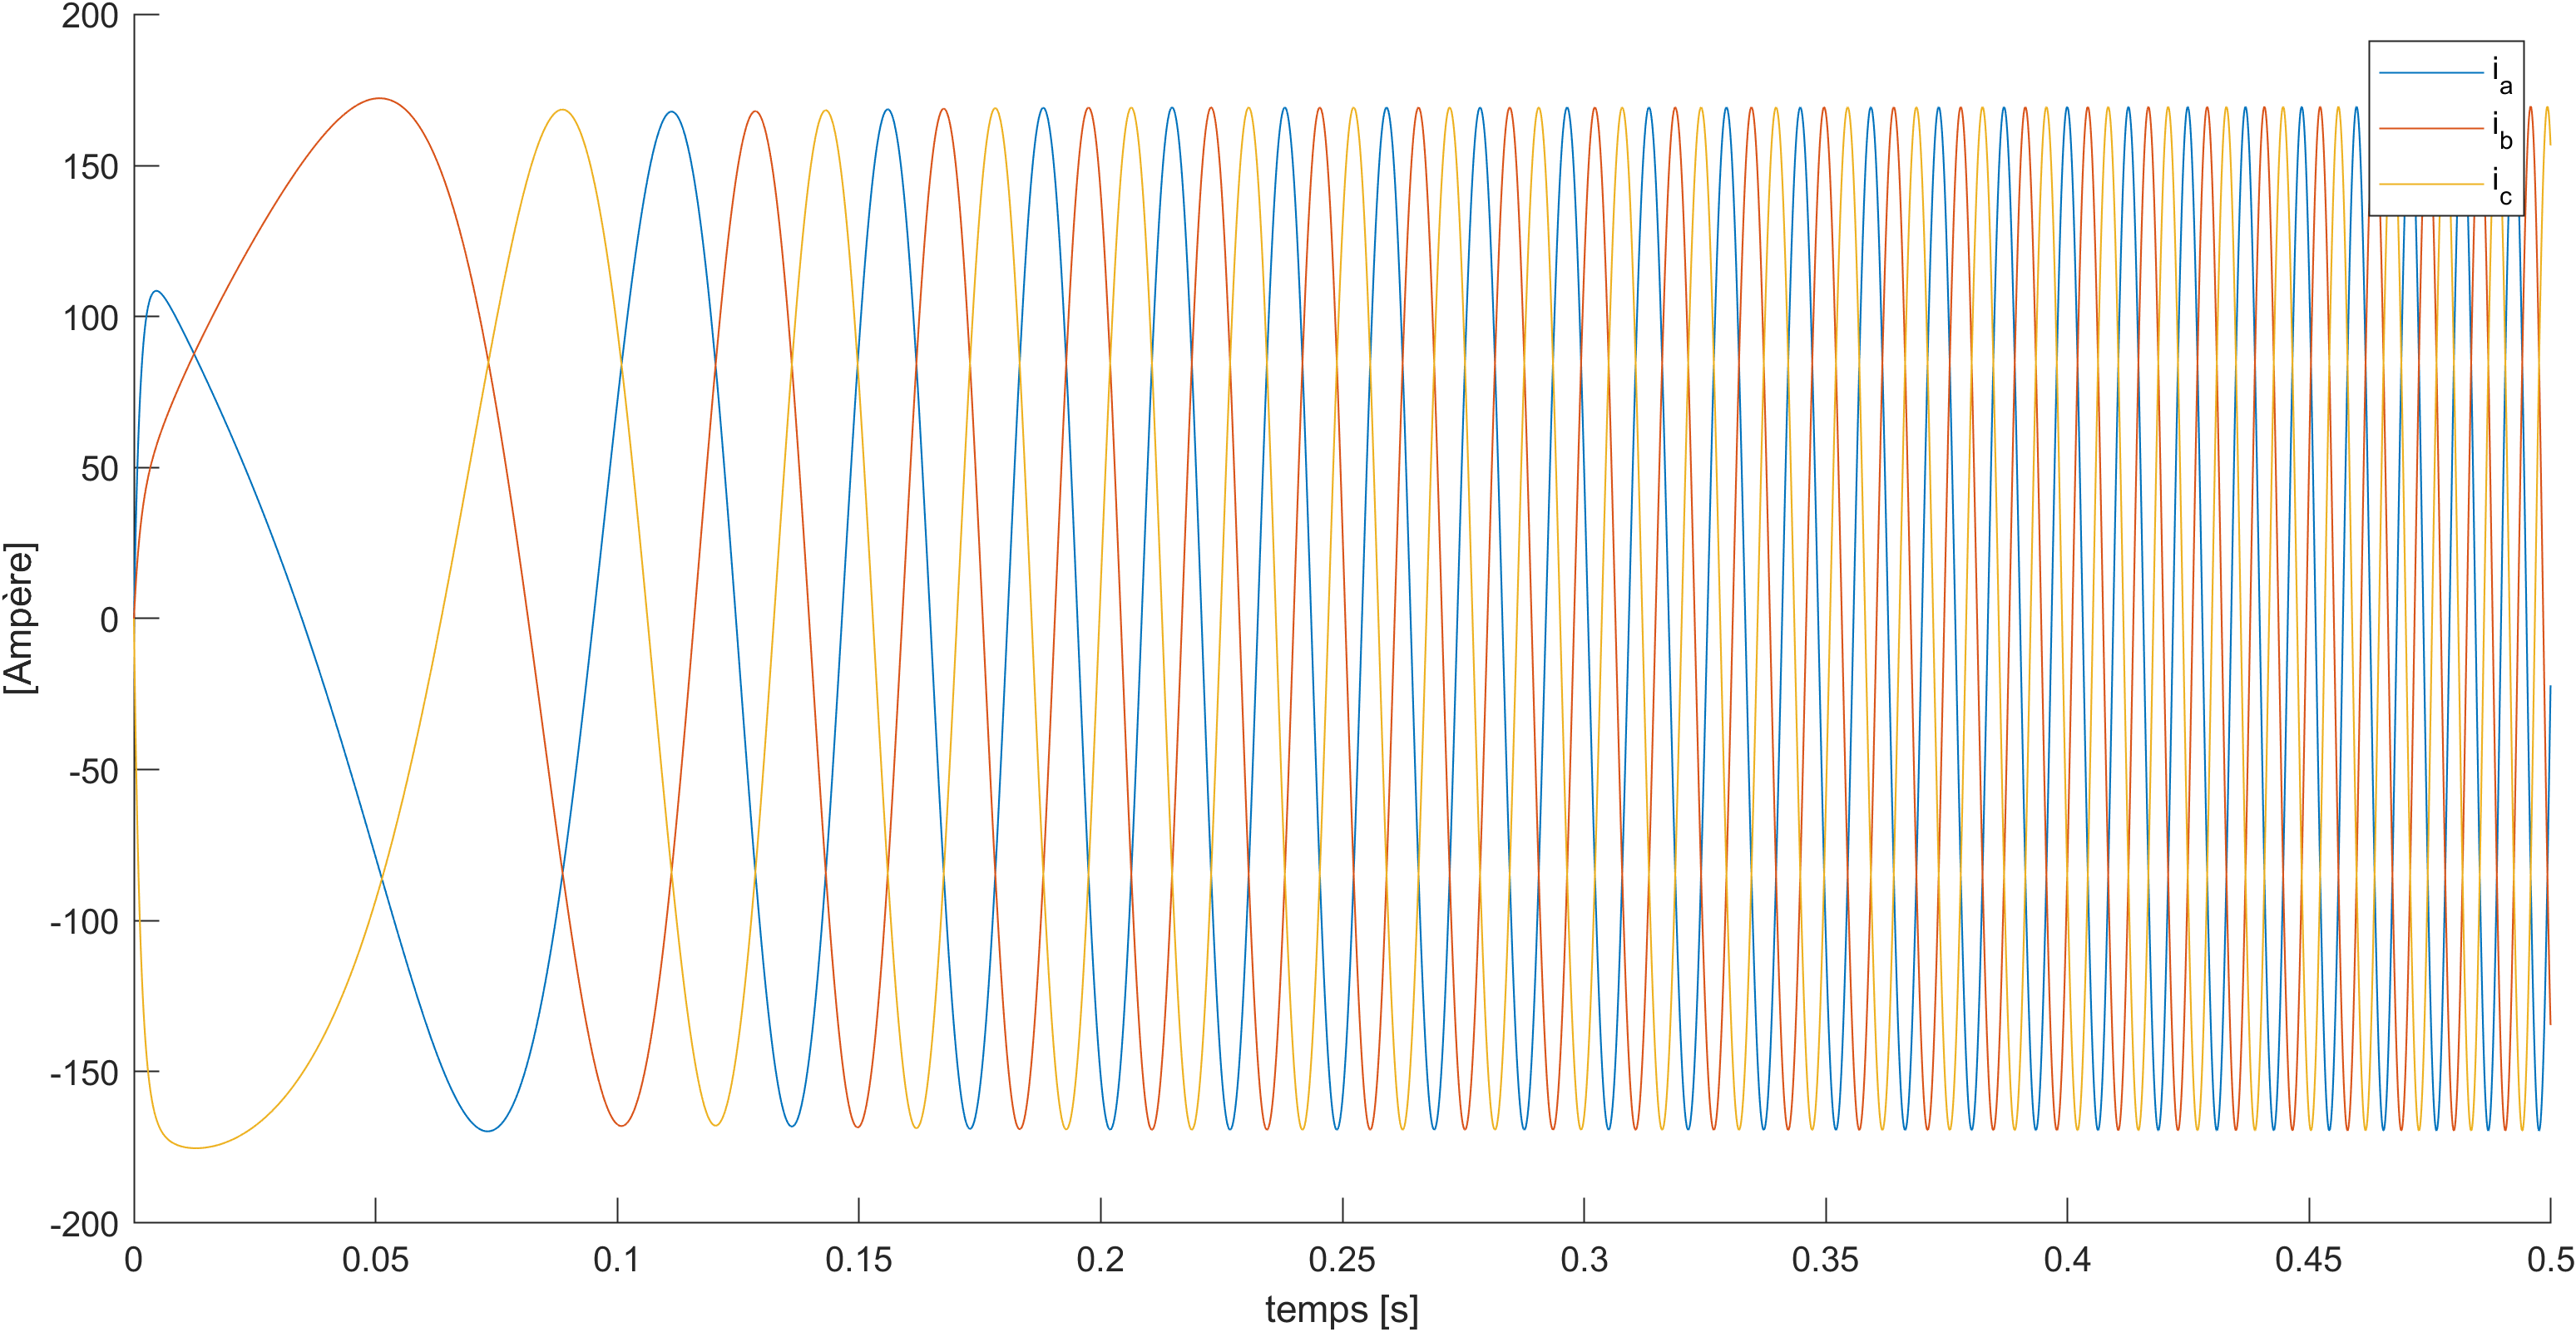
\includegraphics[width=0.8\textwidth]{simusMATLAB/MAS/is_abc.png} 
    \caption{Courants triphasées do stator de la MAS mesurées au cous du temps.}
    \label{img-simuMatlab-is_abc}
\end{figure}

Dans la Figure \ref{img-simuMatlab-is_dq}, un comportement transitoire initial évolue rapidement vers une stabilisation autour de la valeur cible de 150 A, illustrant l'efficacité du contrôle exercé sur le système :


\begin{figure}[!h]
    \centering
    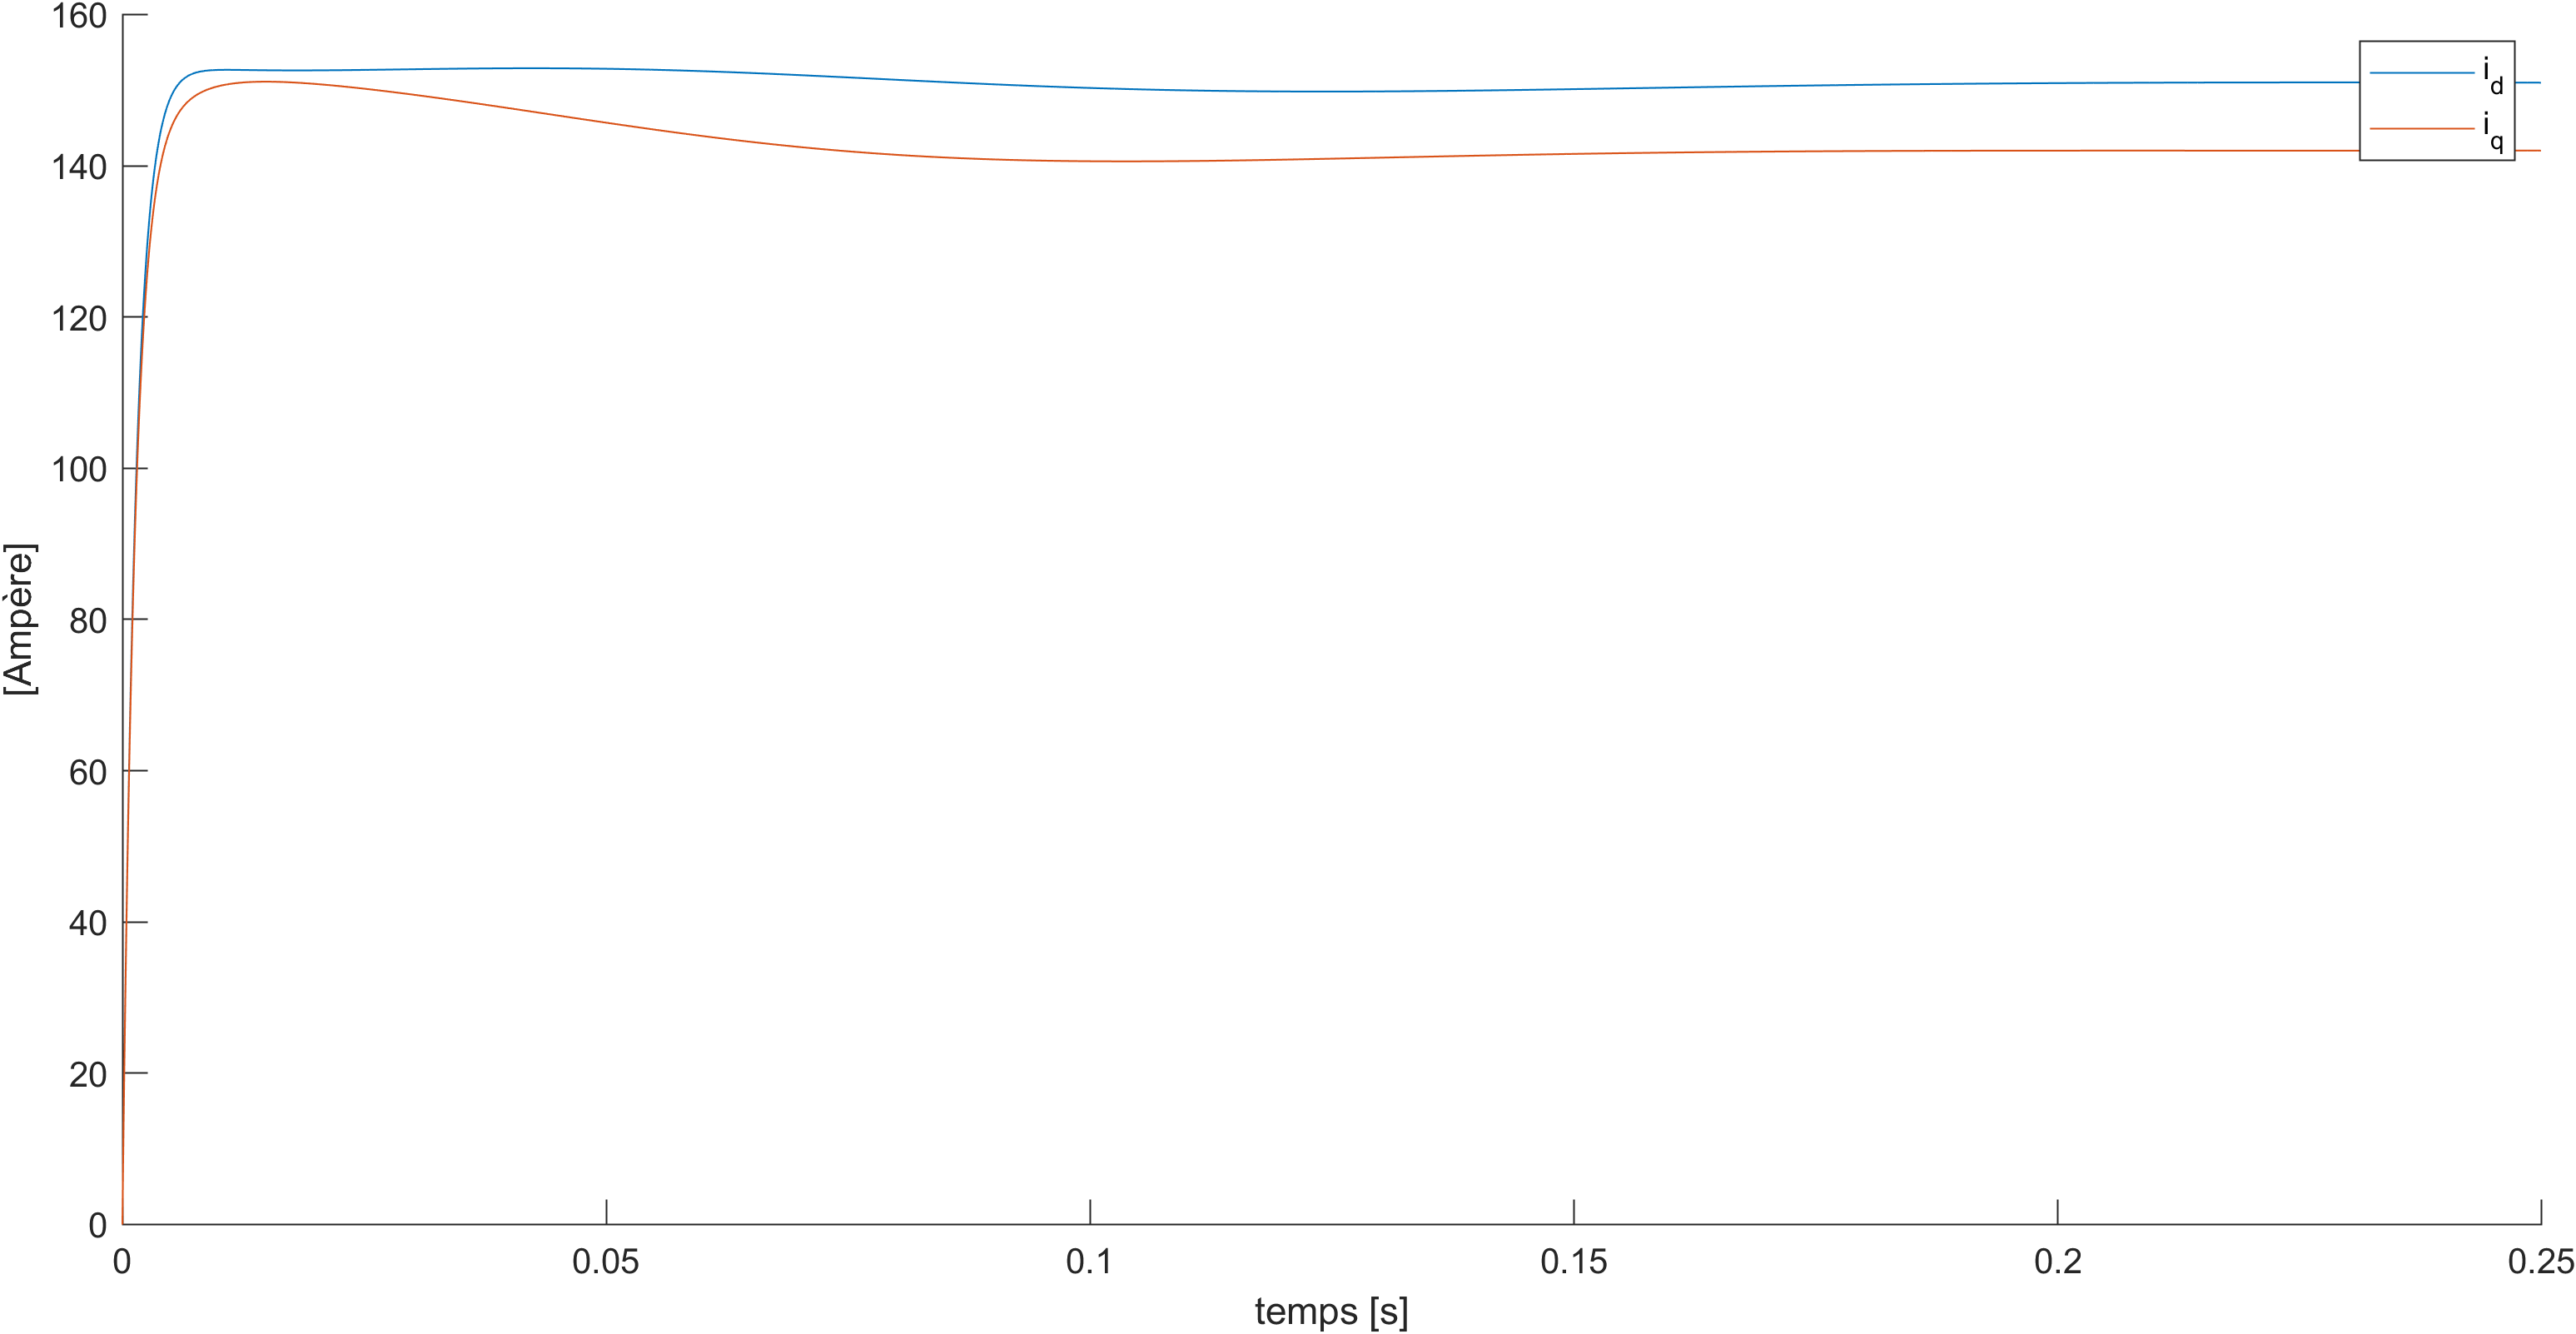
\includegraphics[width=0.8\textwidth]{simusMATLAB/MAS/is_dq.png} 
    \caption{Courants dans le repère dq du stator de la MAS au cous du temps.}
    \label{img-simuMatlab-is_dq}
\end{figure}


La comparaison entre les figures \ref{img-simuMatlab-is_dq} et \ref{img-simuMatlab-is_alphabeta} illustre efficacement la validité de la transformation de Park. Elle démontre visuellement comment les courants dans le repère dq sont affectés par la variation de fréquence \(\theta_s\), offrant une perspective claire sur la dynamique des courants sous cette transformation.


\begin{figure}[!h]
    \centering
    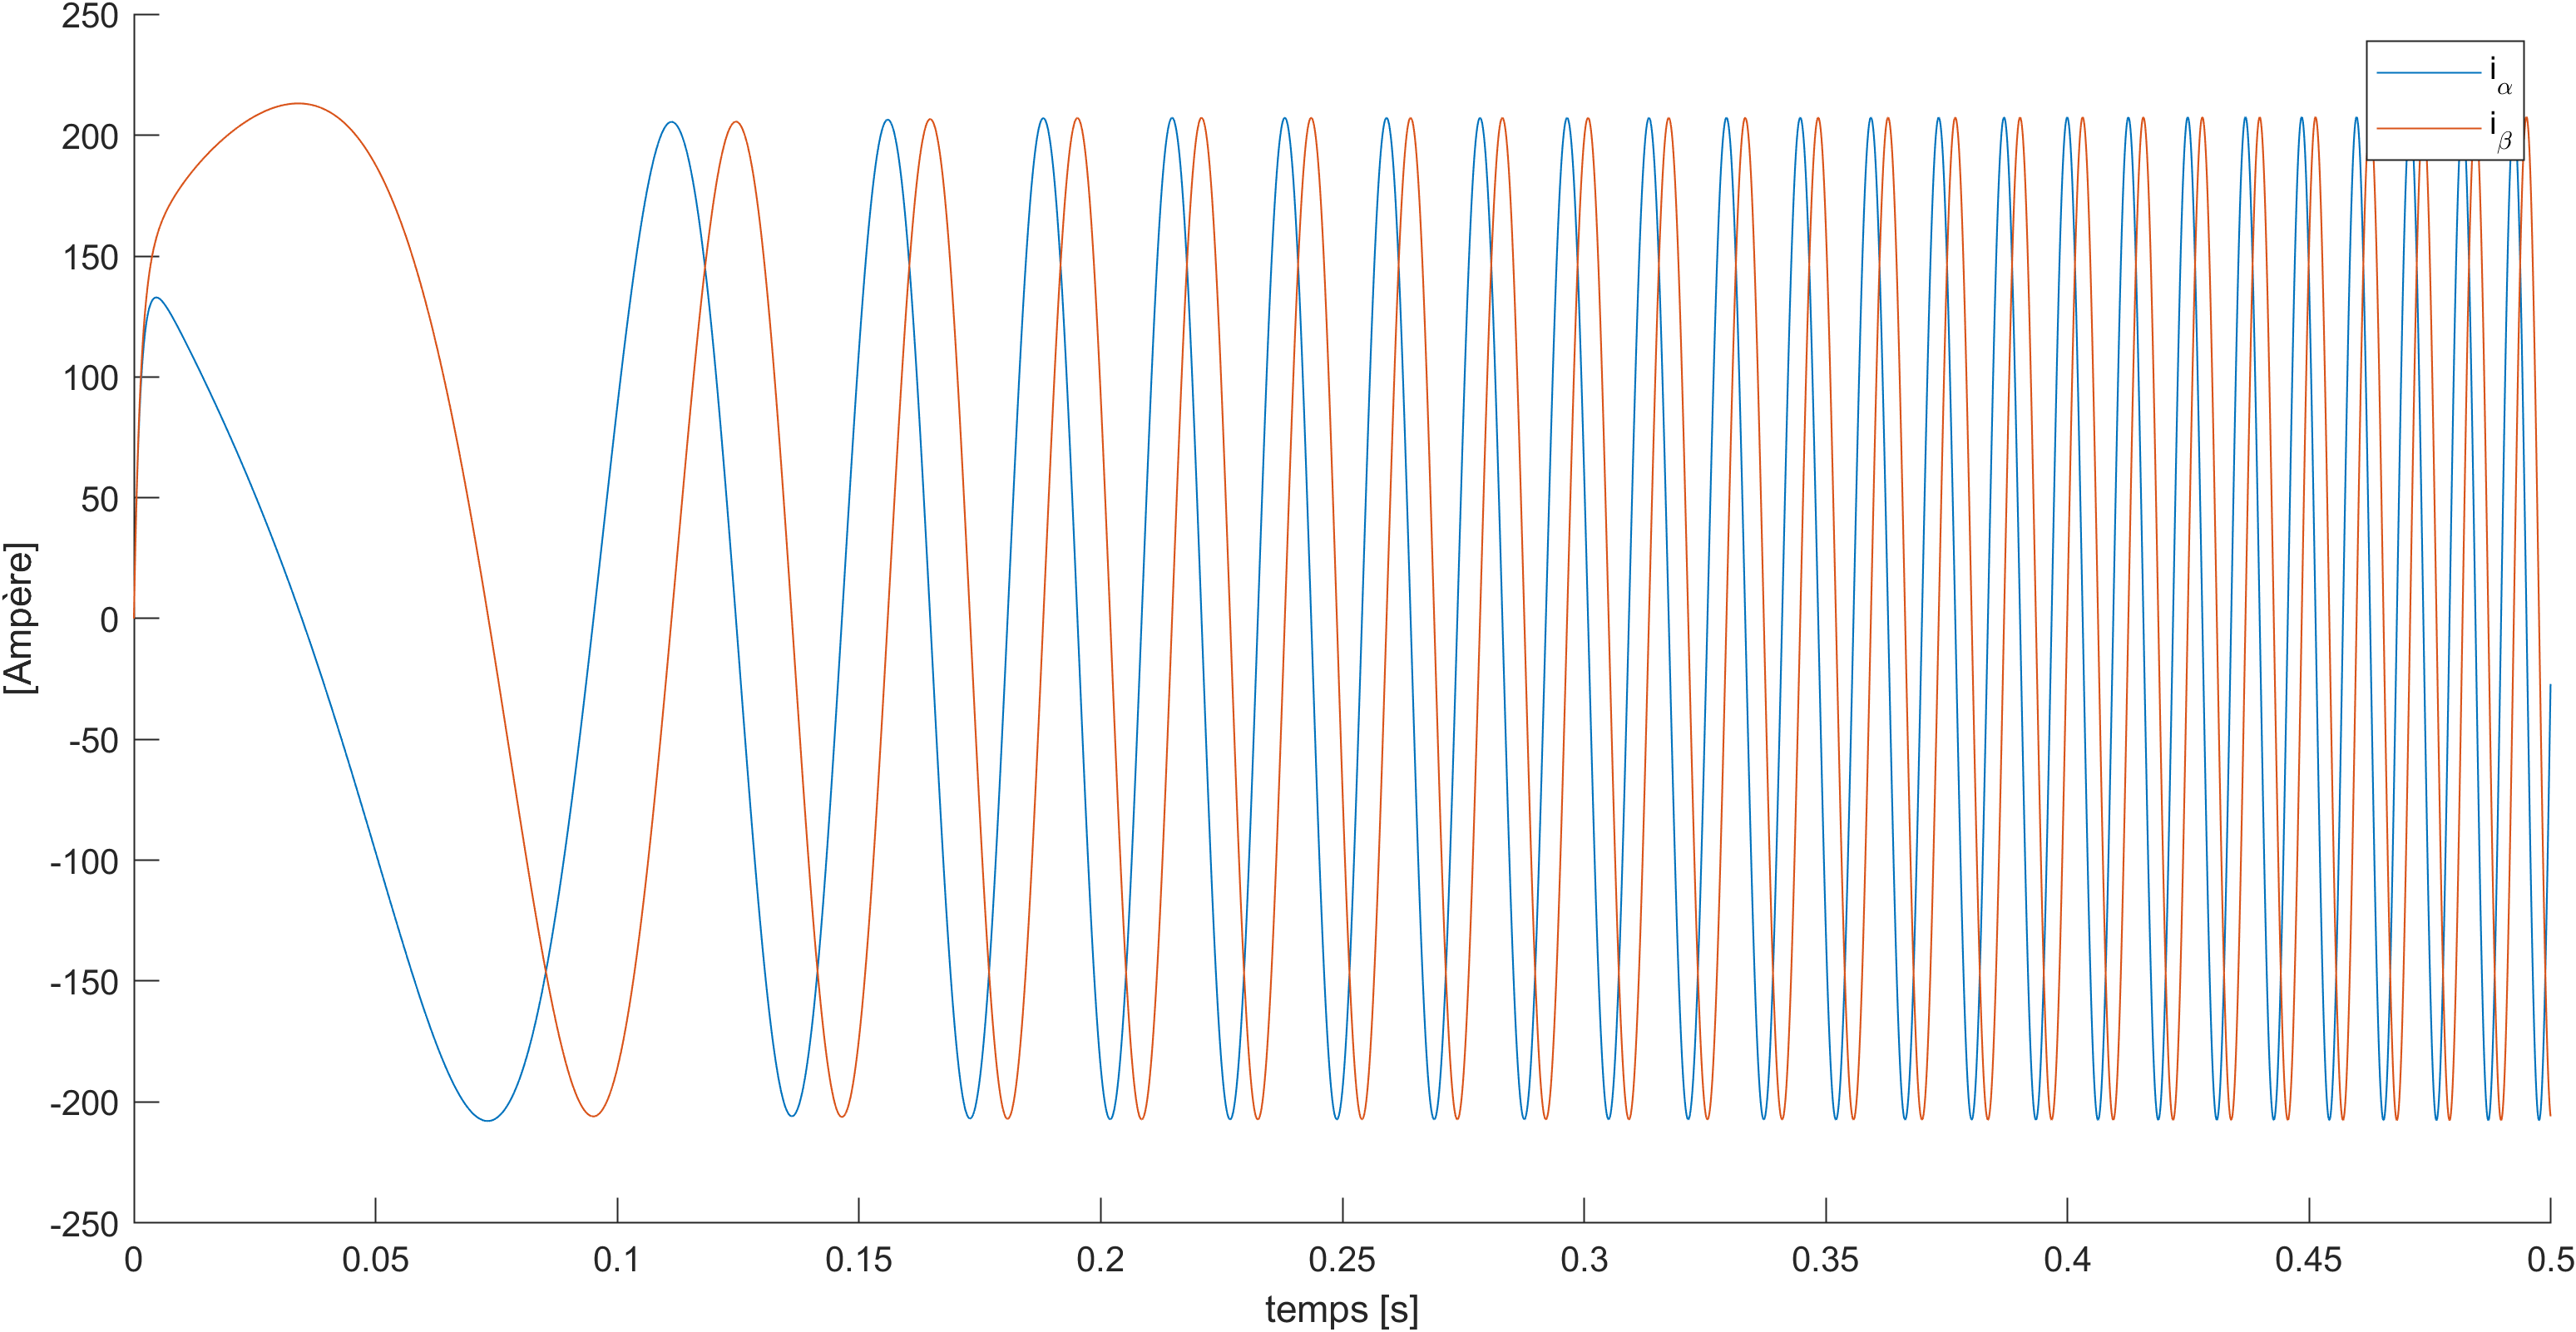
\includegraphics[width=0.8\textwidth]{simusMATLAB/MAS/is_alphabeta.png} 
    \caption{Courants dans le repère $\alpha\beta$ du stator de la machine au cous du temps.}
    \label{img-simuMatlab-is_alphabeta}
\end{figure}

L'analyse des données du stator de la machine asynchrone simulée révèle un comportement cohérent pour les tensions, similaire à celui observé pour les courants. La Figure \ref{img-simuMatlab-vs_abc} illustre les tensions triphasées, tandis que \ref{img-simuMatlab-Vs_dq} présente ces tensions dans le repère dq. La transformation de Park, appliquée en utilisant l'angle variable du stator, est validée par ces observations, comme le montre la Figure \ref{img-simuMatlab-Vs_alphabeta}, démontrant la conversion des tensions en suivant la fréquence de rotation \(\theta_s\).


\begin{figure}[!h]
    \centering
    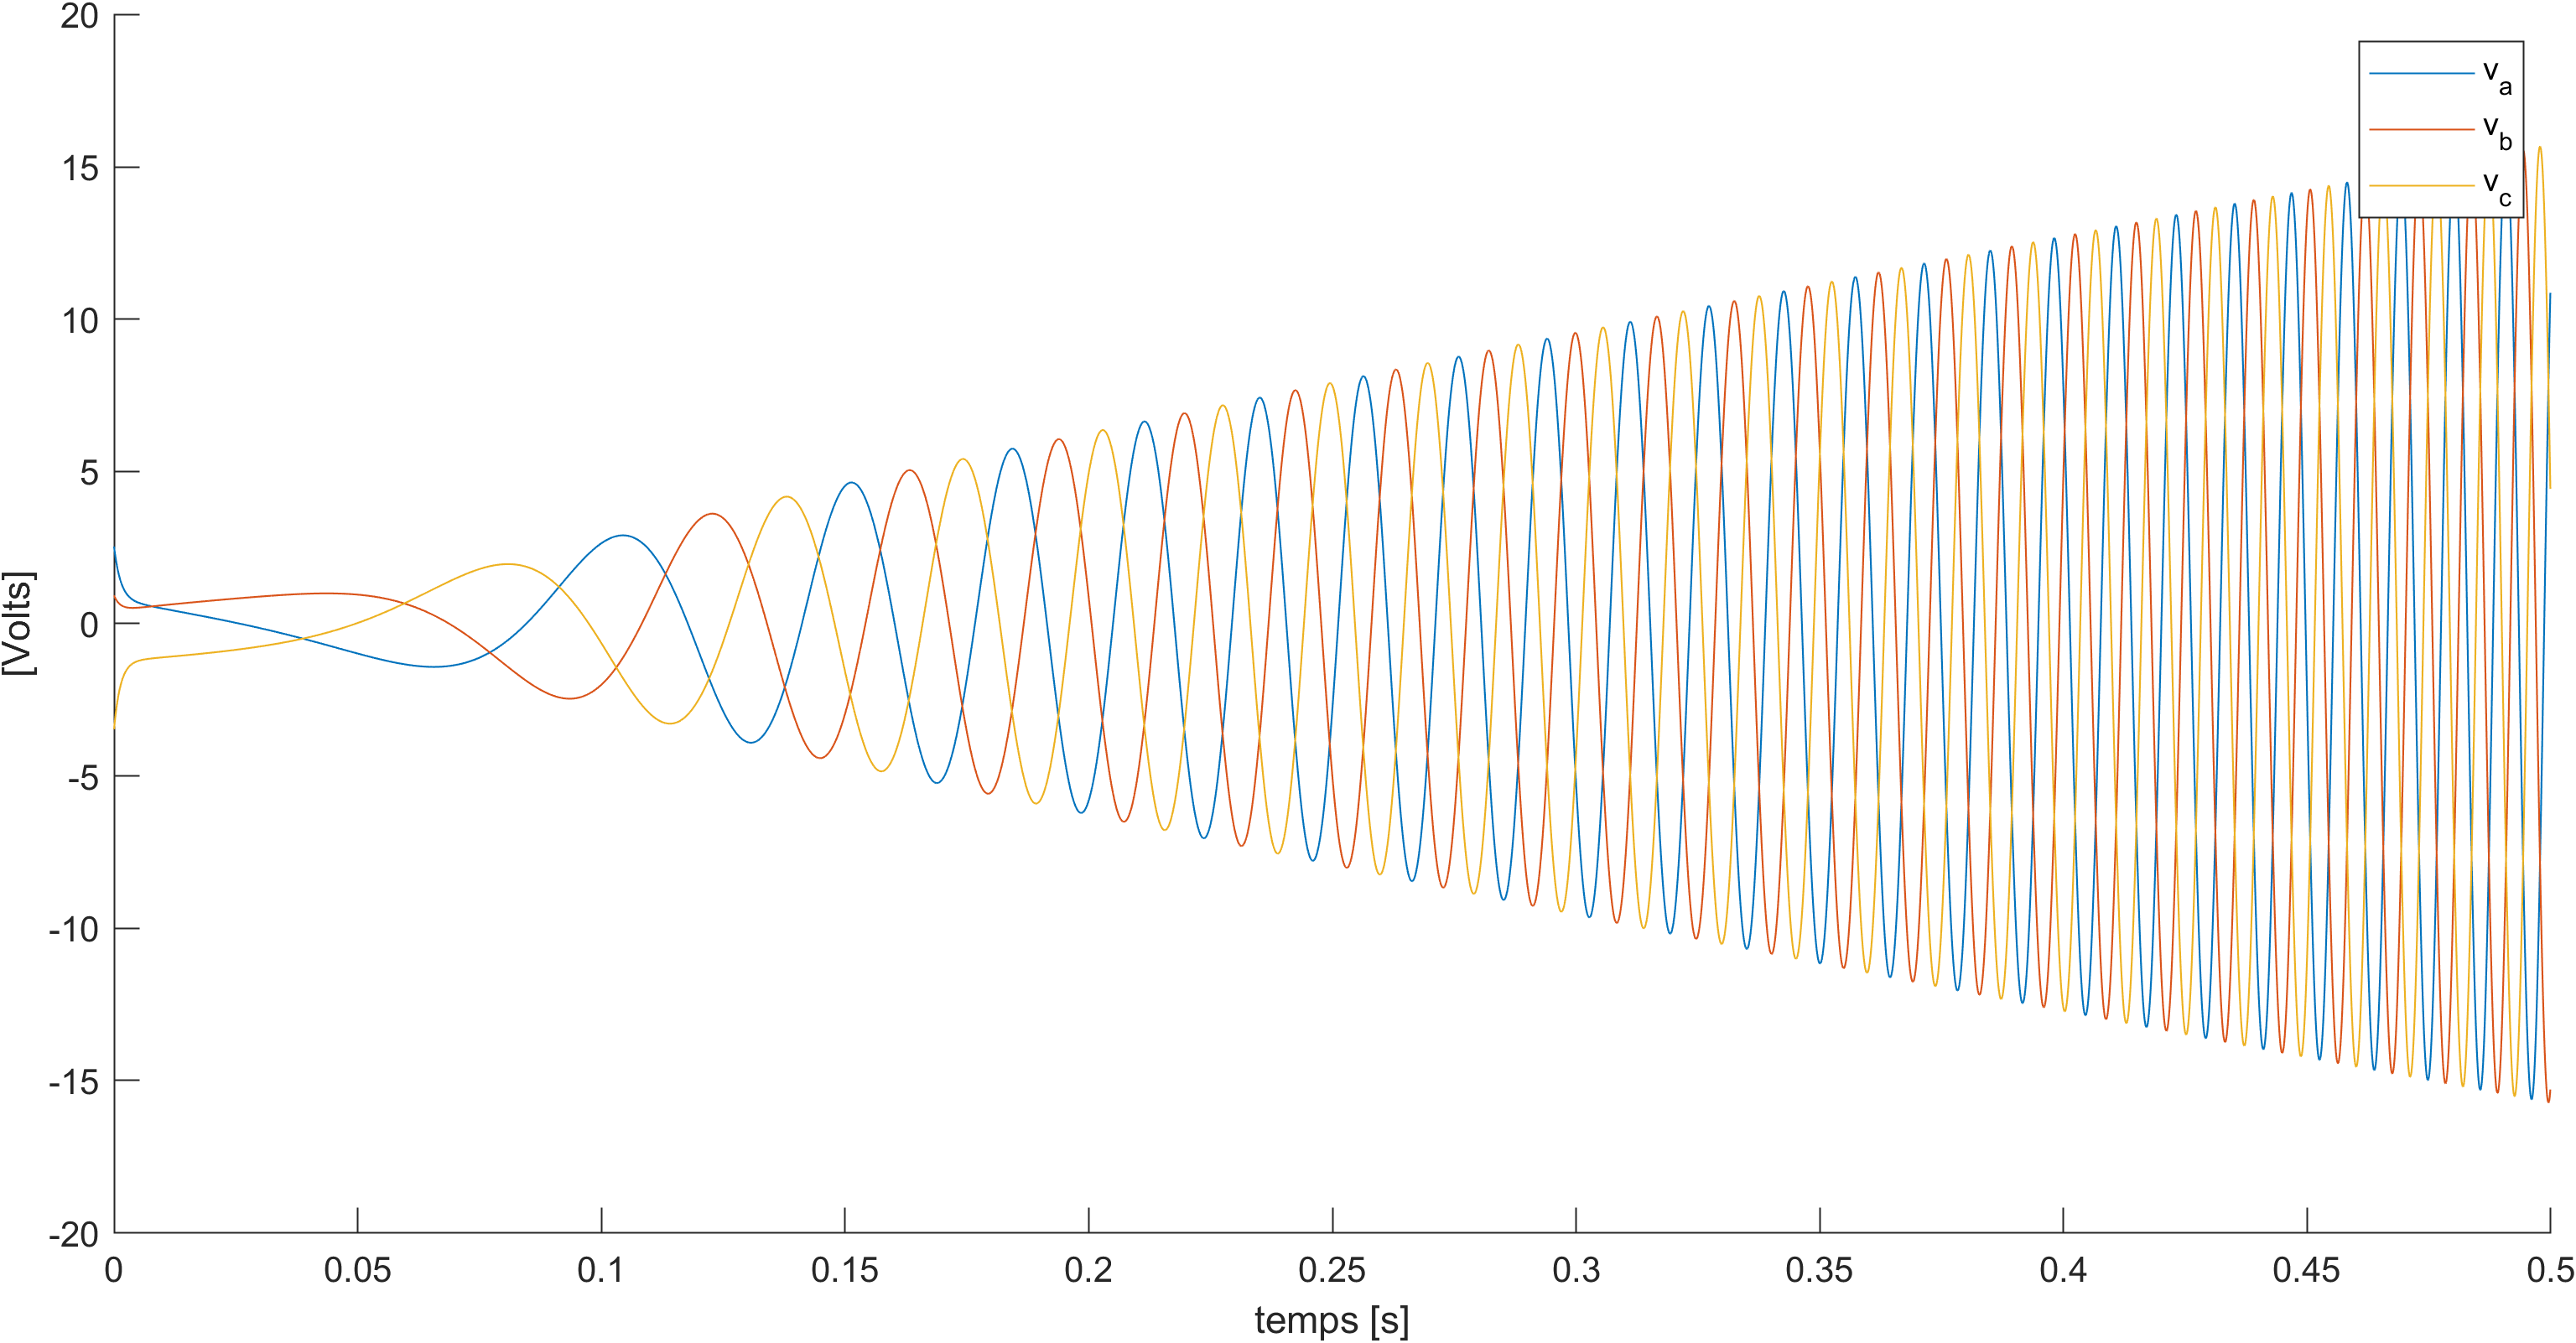
\includegraphics[width=0.8\textwidth]{simusMATLAB/MAS/vs_abc.png} 
    \caption{Tensions triphasées du stator de la MAS mesurées au cous du temps.}
    \label{img-simuMatlab-vs_abc}
\end{figure}

\begin{figure}[!h]
    \centering
    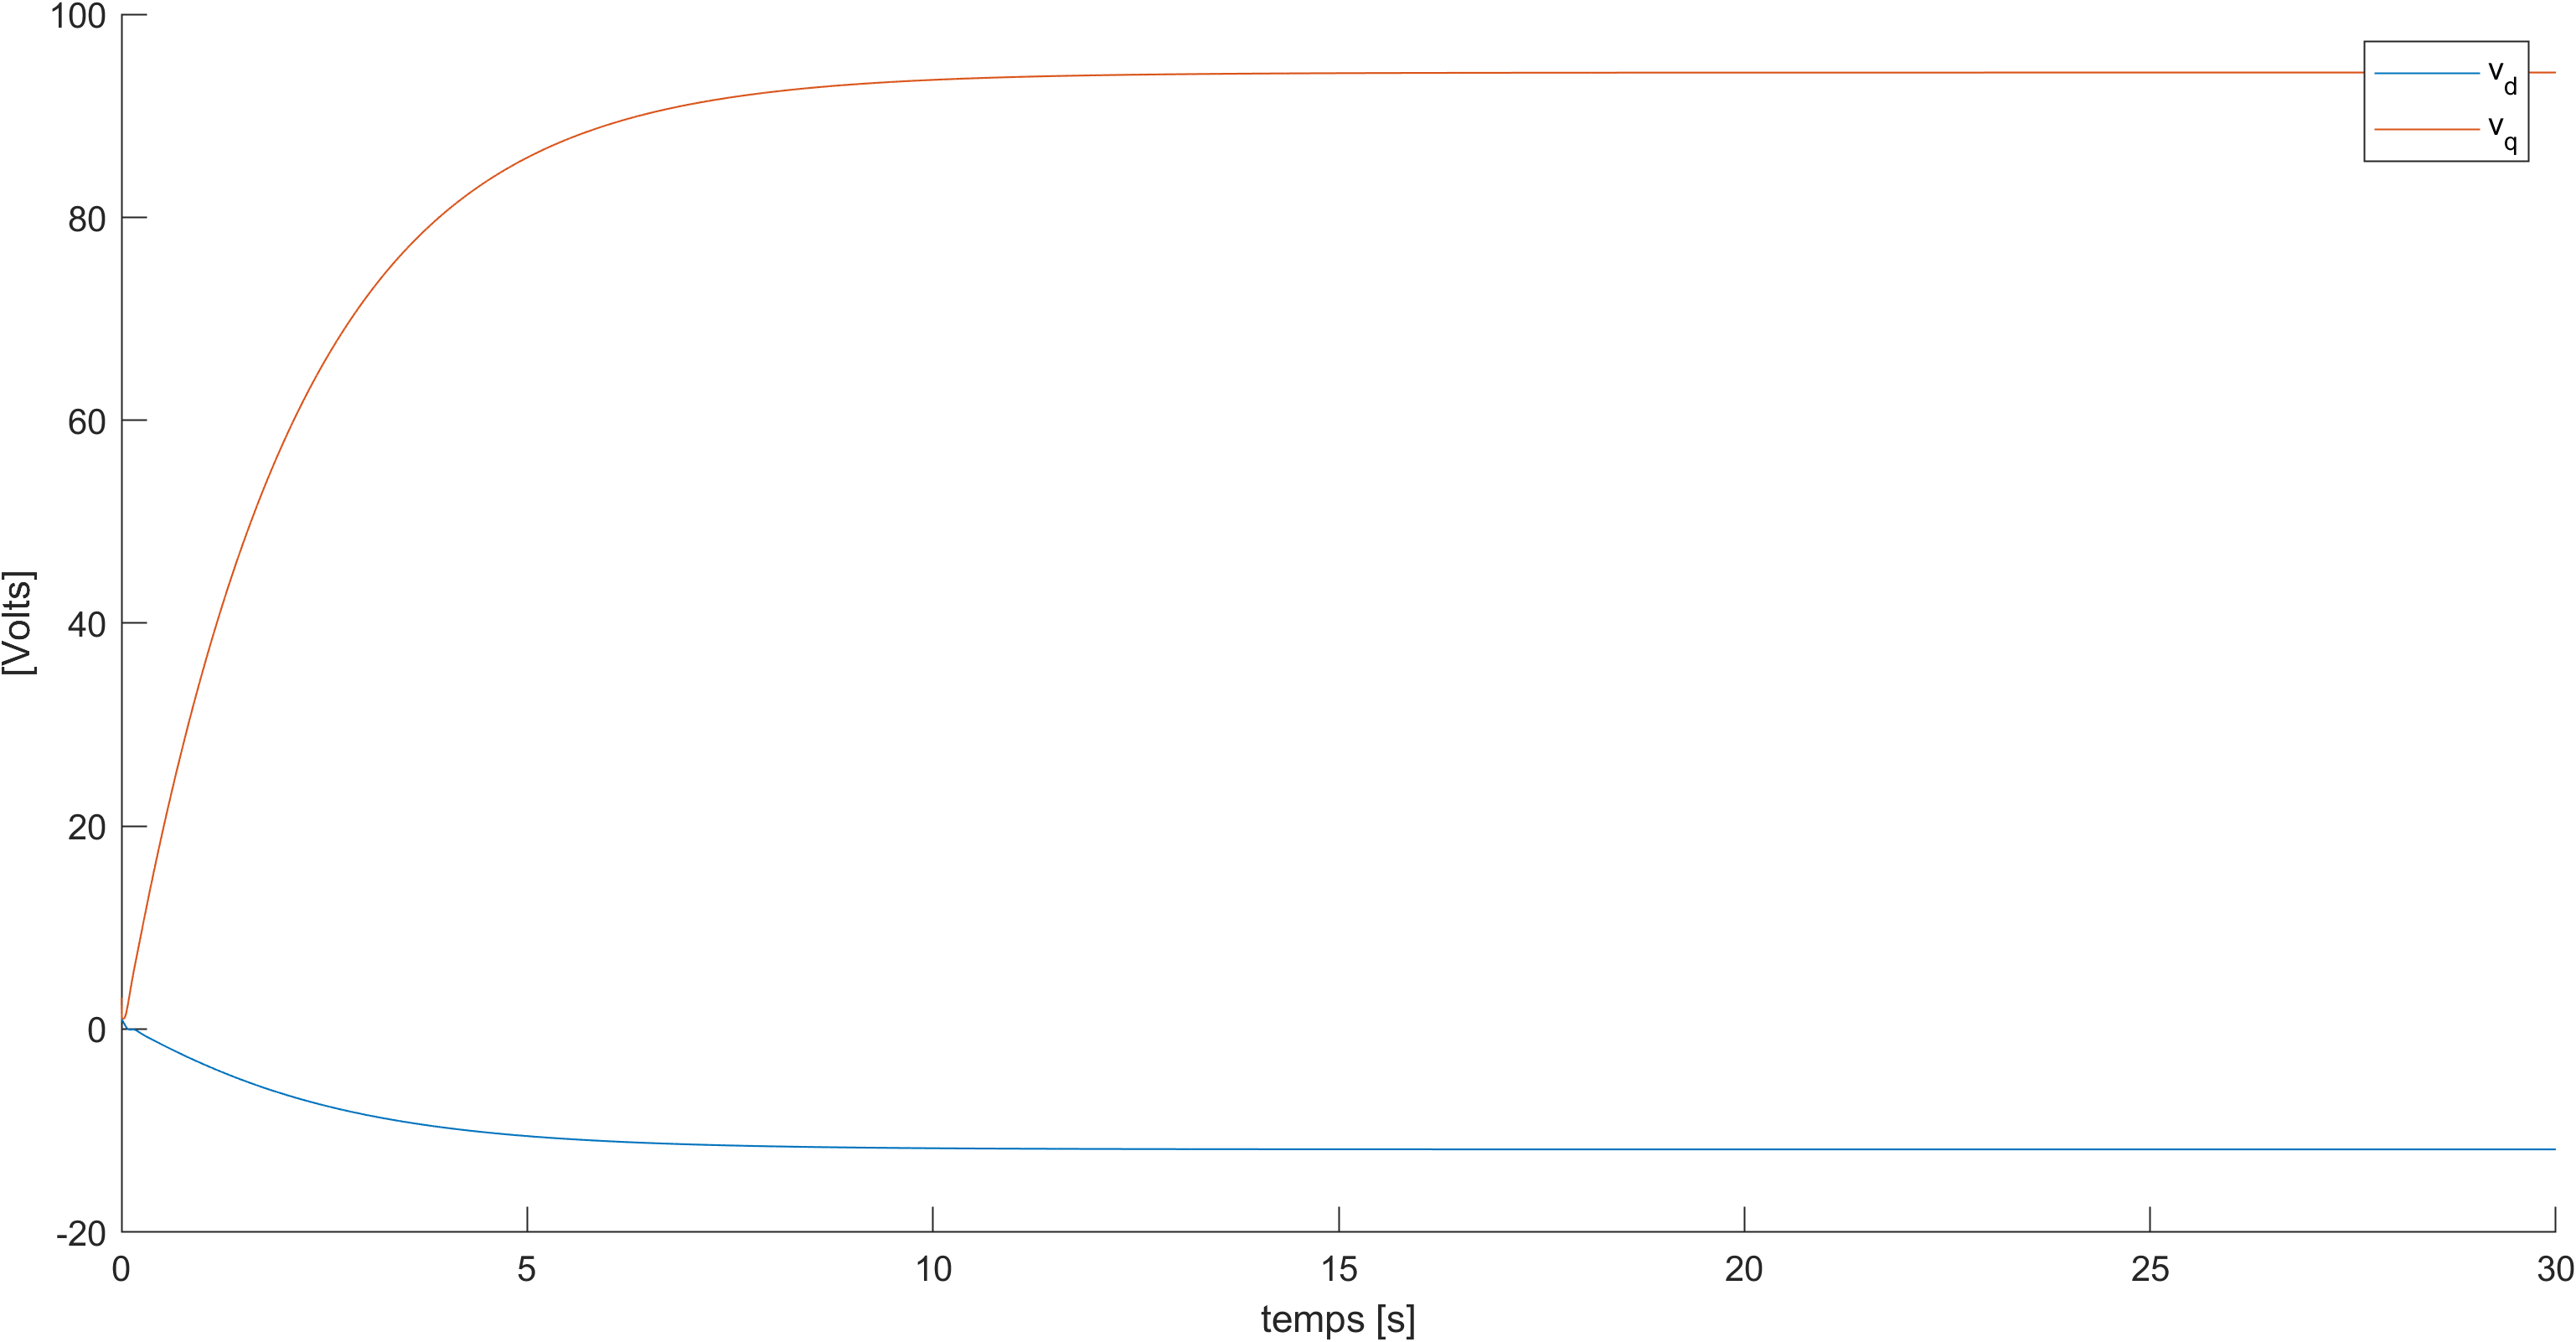
\includegraphics[width=0.8\textwidth]{simusMATLAB/MAS/Vs_dq.png} 
    \caption{Tensions dans le repère dq du stator de la MAS mesurées au cous du temps.}
    \label{img-simuMatlab-Vs_dq}
\end{figure}


\begin{figure}[!h]
    \centering
    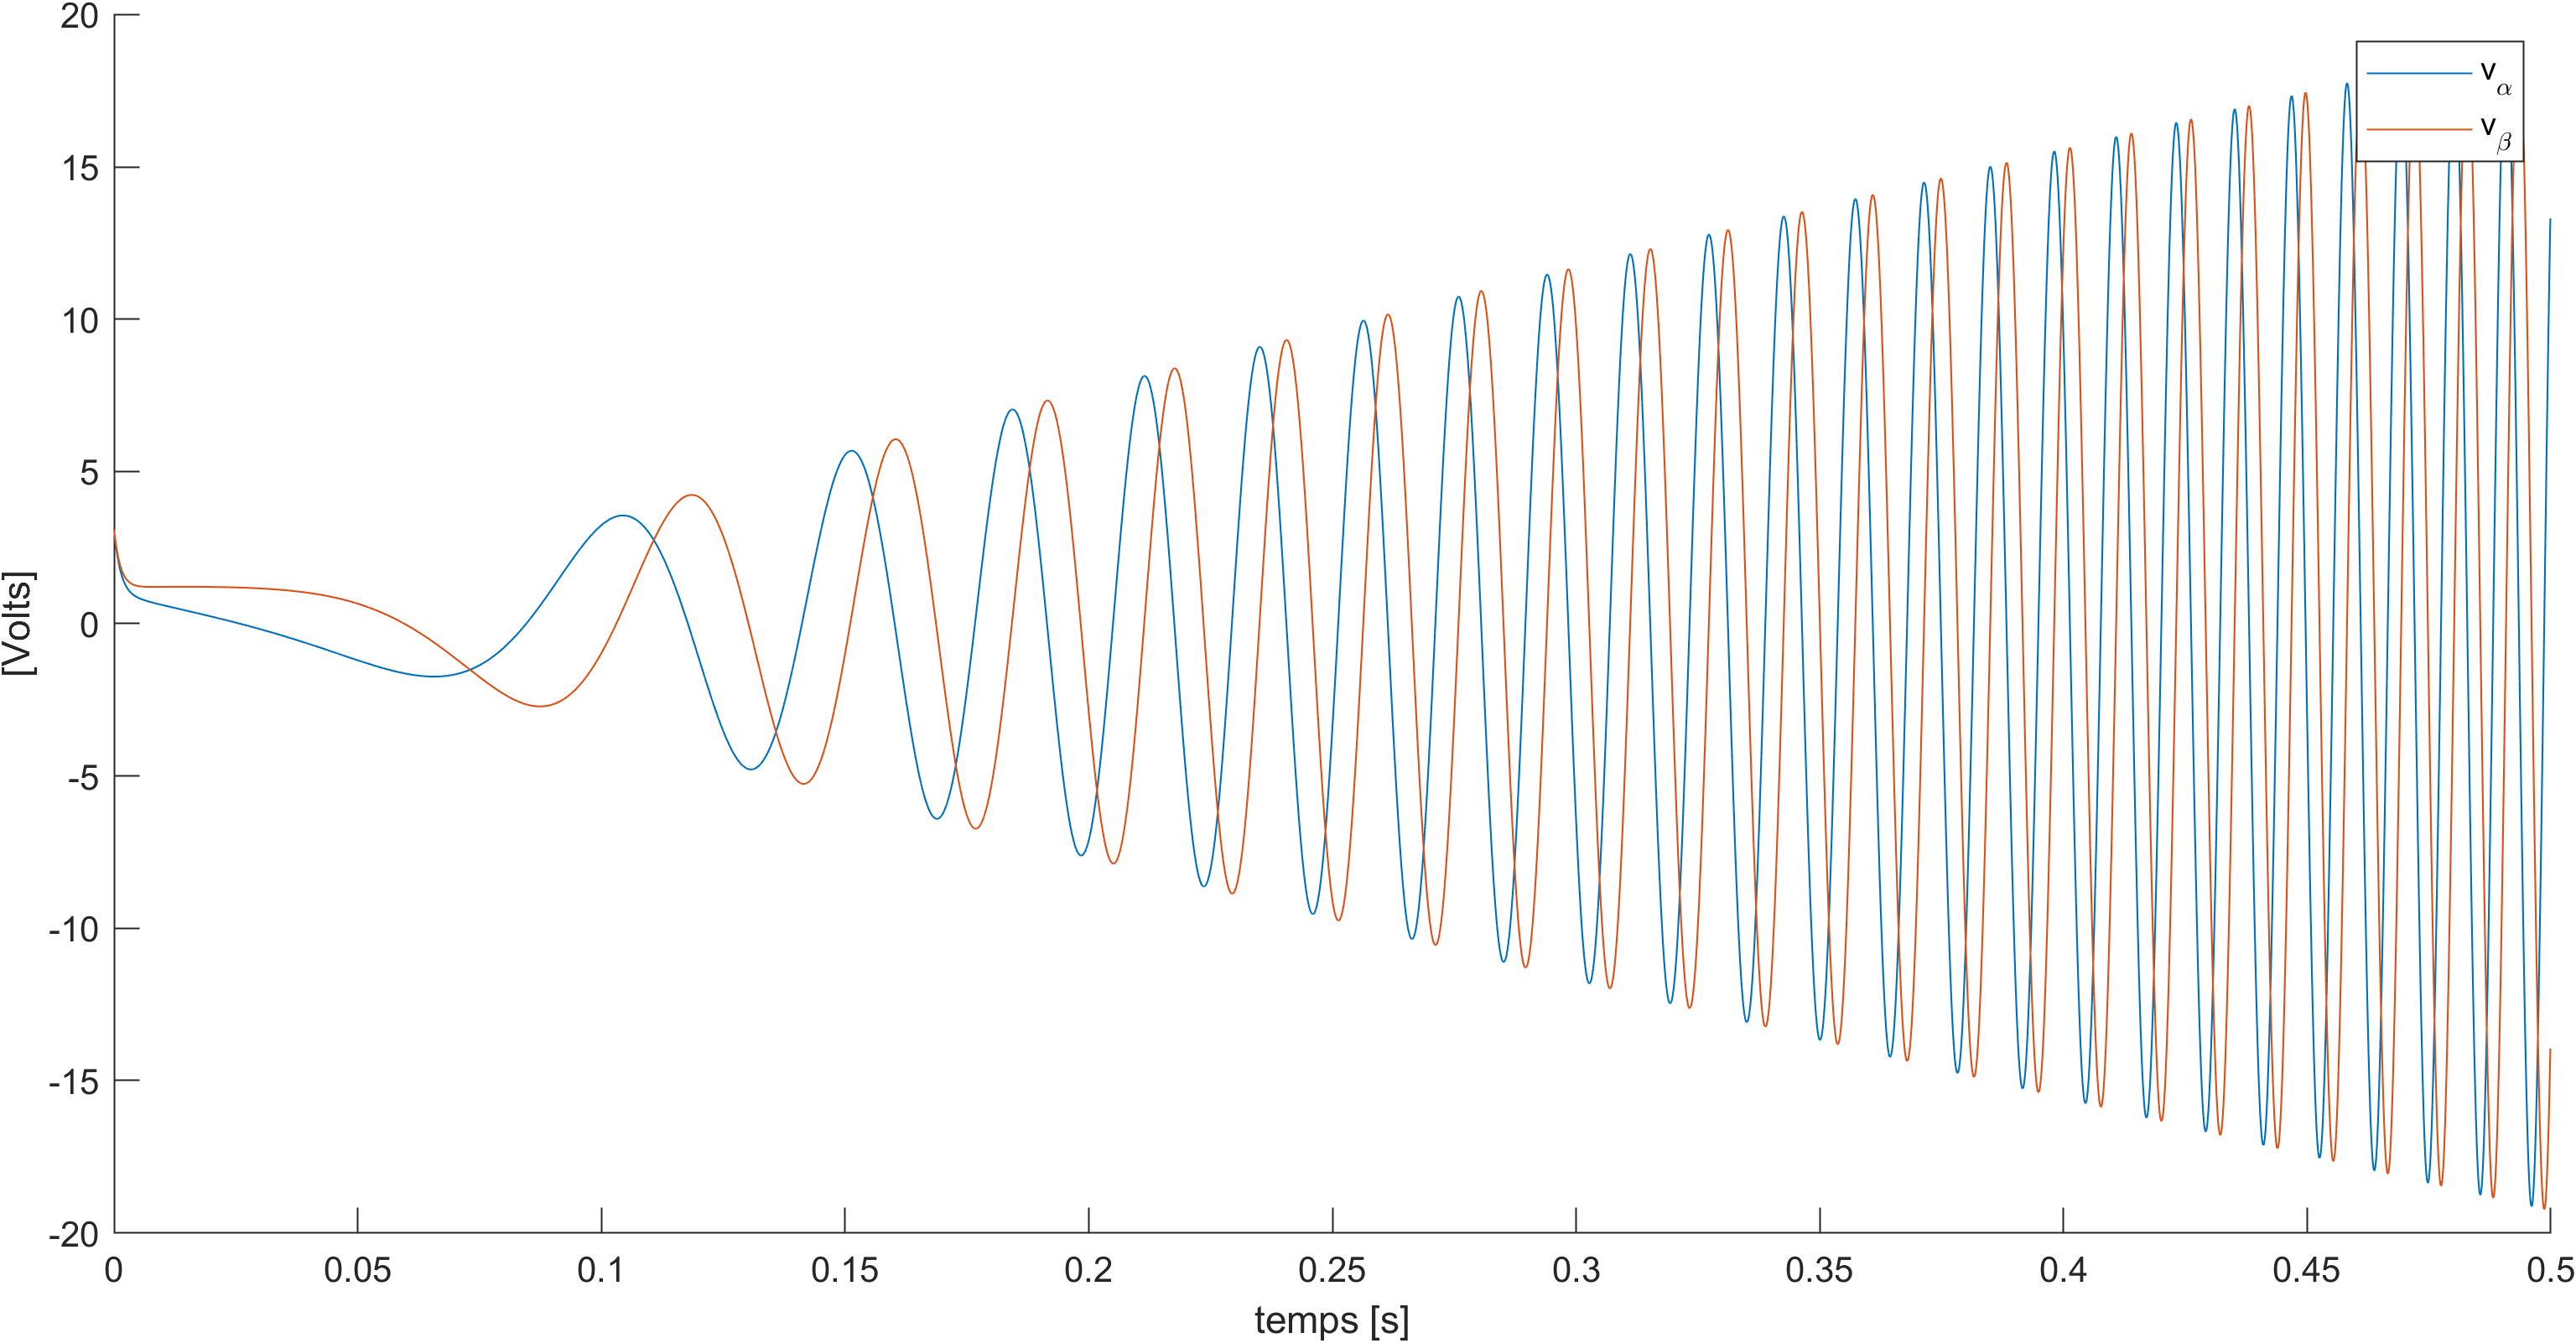
\includegraphics[width=0.8\textwidth]{simusMATLAB/MAS/Vs_alphabeta.png} 
    \caption{Tensions dans le repère $\alpha\beta$ du stator de la MAS mesurées au cous du temps.}
    \label{img-simuMatlab-Vs_alphabeta}
\end{figure}

Pour approfondir la compréhension de la variation angulaire au fil du temps, une analyse de \(\theta_s\) et \(\theta_r\) révèle une augmentation progressive de \(\theta_s\) alors que \(\theta_r\) reste inchangé, reflétant l'absence d'alimentation électrique au rotor. Cette dynamique est clairement exposée, soulignant l'effet de l'alimentation statorique sur la variation angulaire sur la Figure \ref{img-simuMatlab-thetas}.


\begin{figure}[!h]
    \centering
    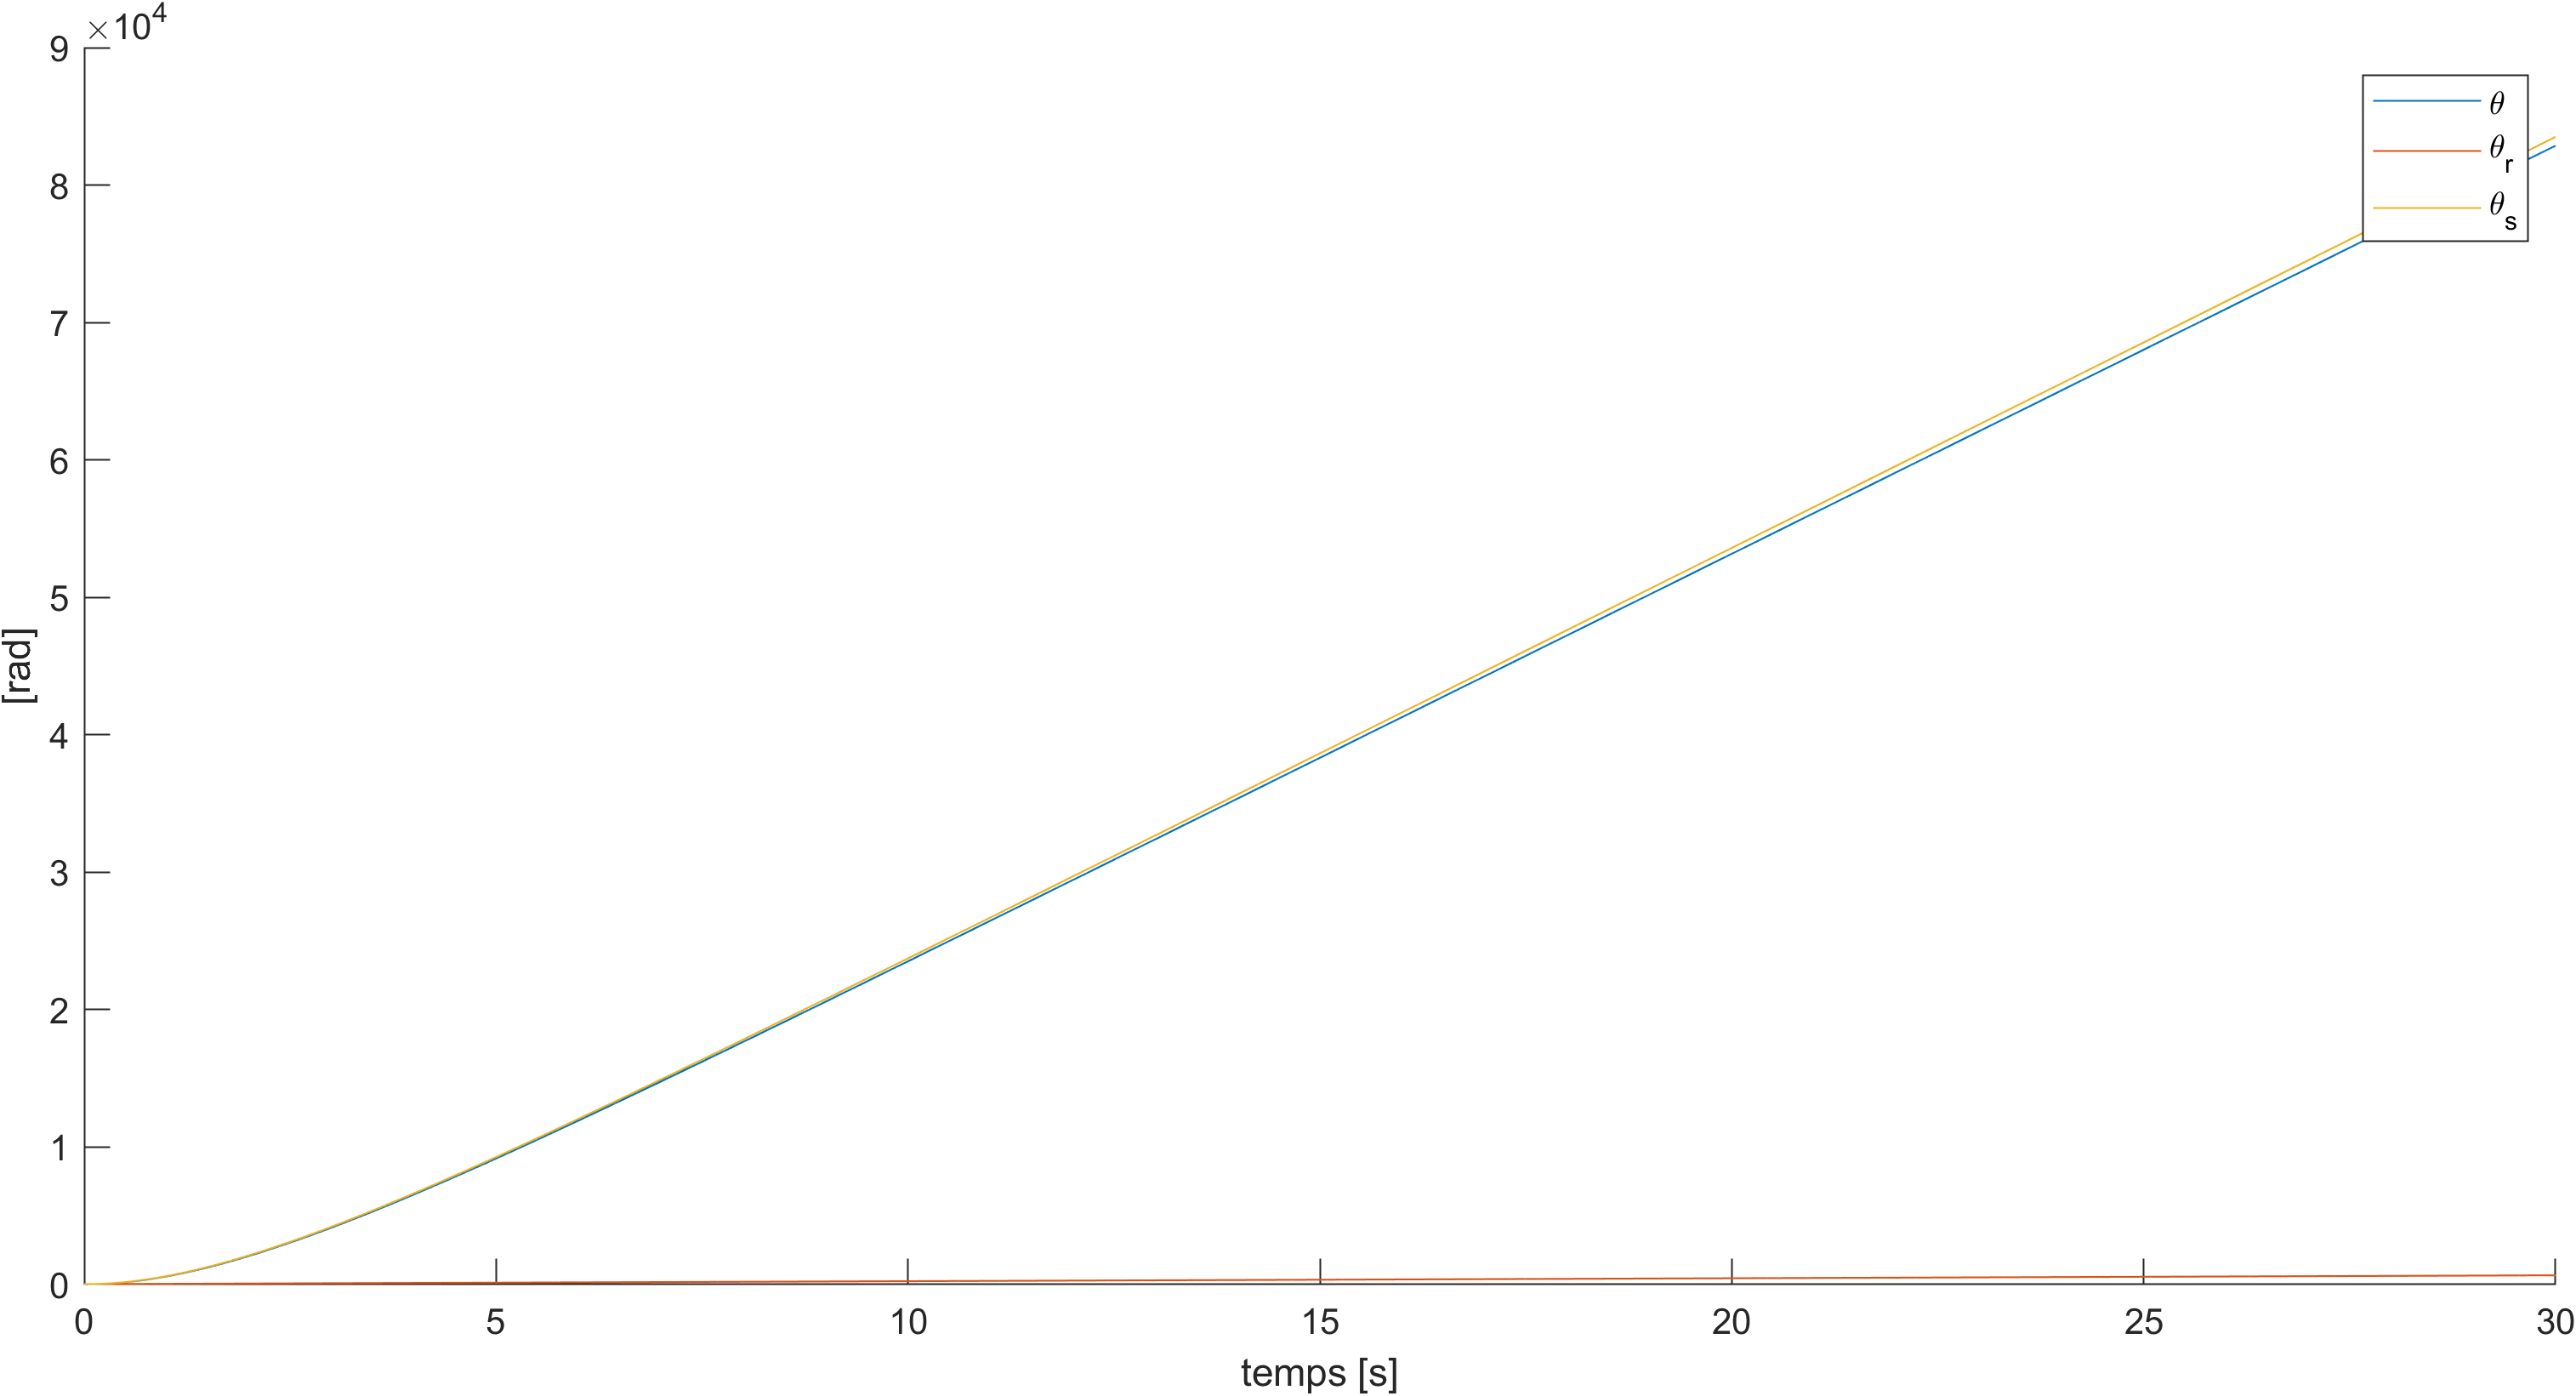
\includegraphics[width=0.8\textwidth]{simusMATLAB/MAS/thetas.png} 
    \caption{Angles de phase des grandeurs de la MAS mesurée au cous du temps.}
    \label{img-simuMatlab-thetas}
\end{figure}


L'angle \(\theta\), observé dans la Figure \ref{img-simuMatlab-thetas}, permet de visualiser le mouvement des grandeurs rotoriques dans le temps. En appliquant cet angle variable, c'est possible de suivre la rotation des composantes du rotor, illustrant ainsi leur évolution dynamique au fil du temps comme exposée dans les Figures \ref{img-simuMatlab-ir_abc} et \ref{img-simuMatlab-ir_dq}.


\begin{figure}[!h]
    \centering
    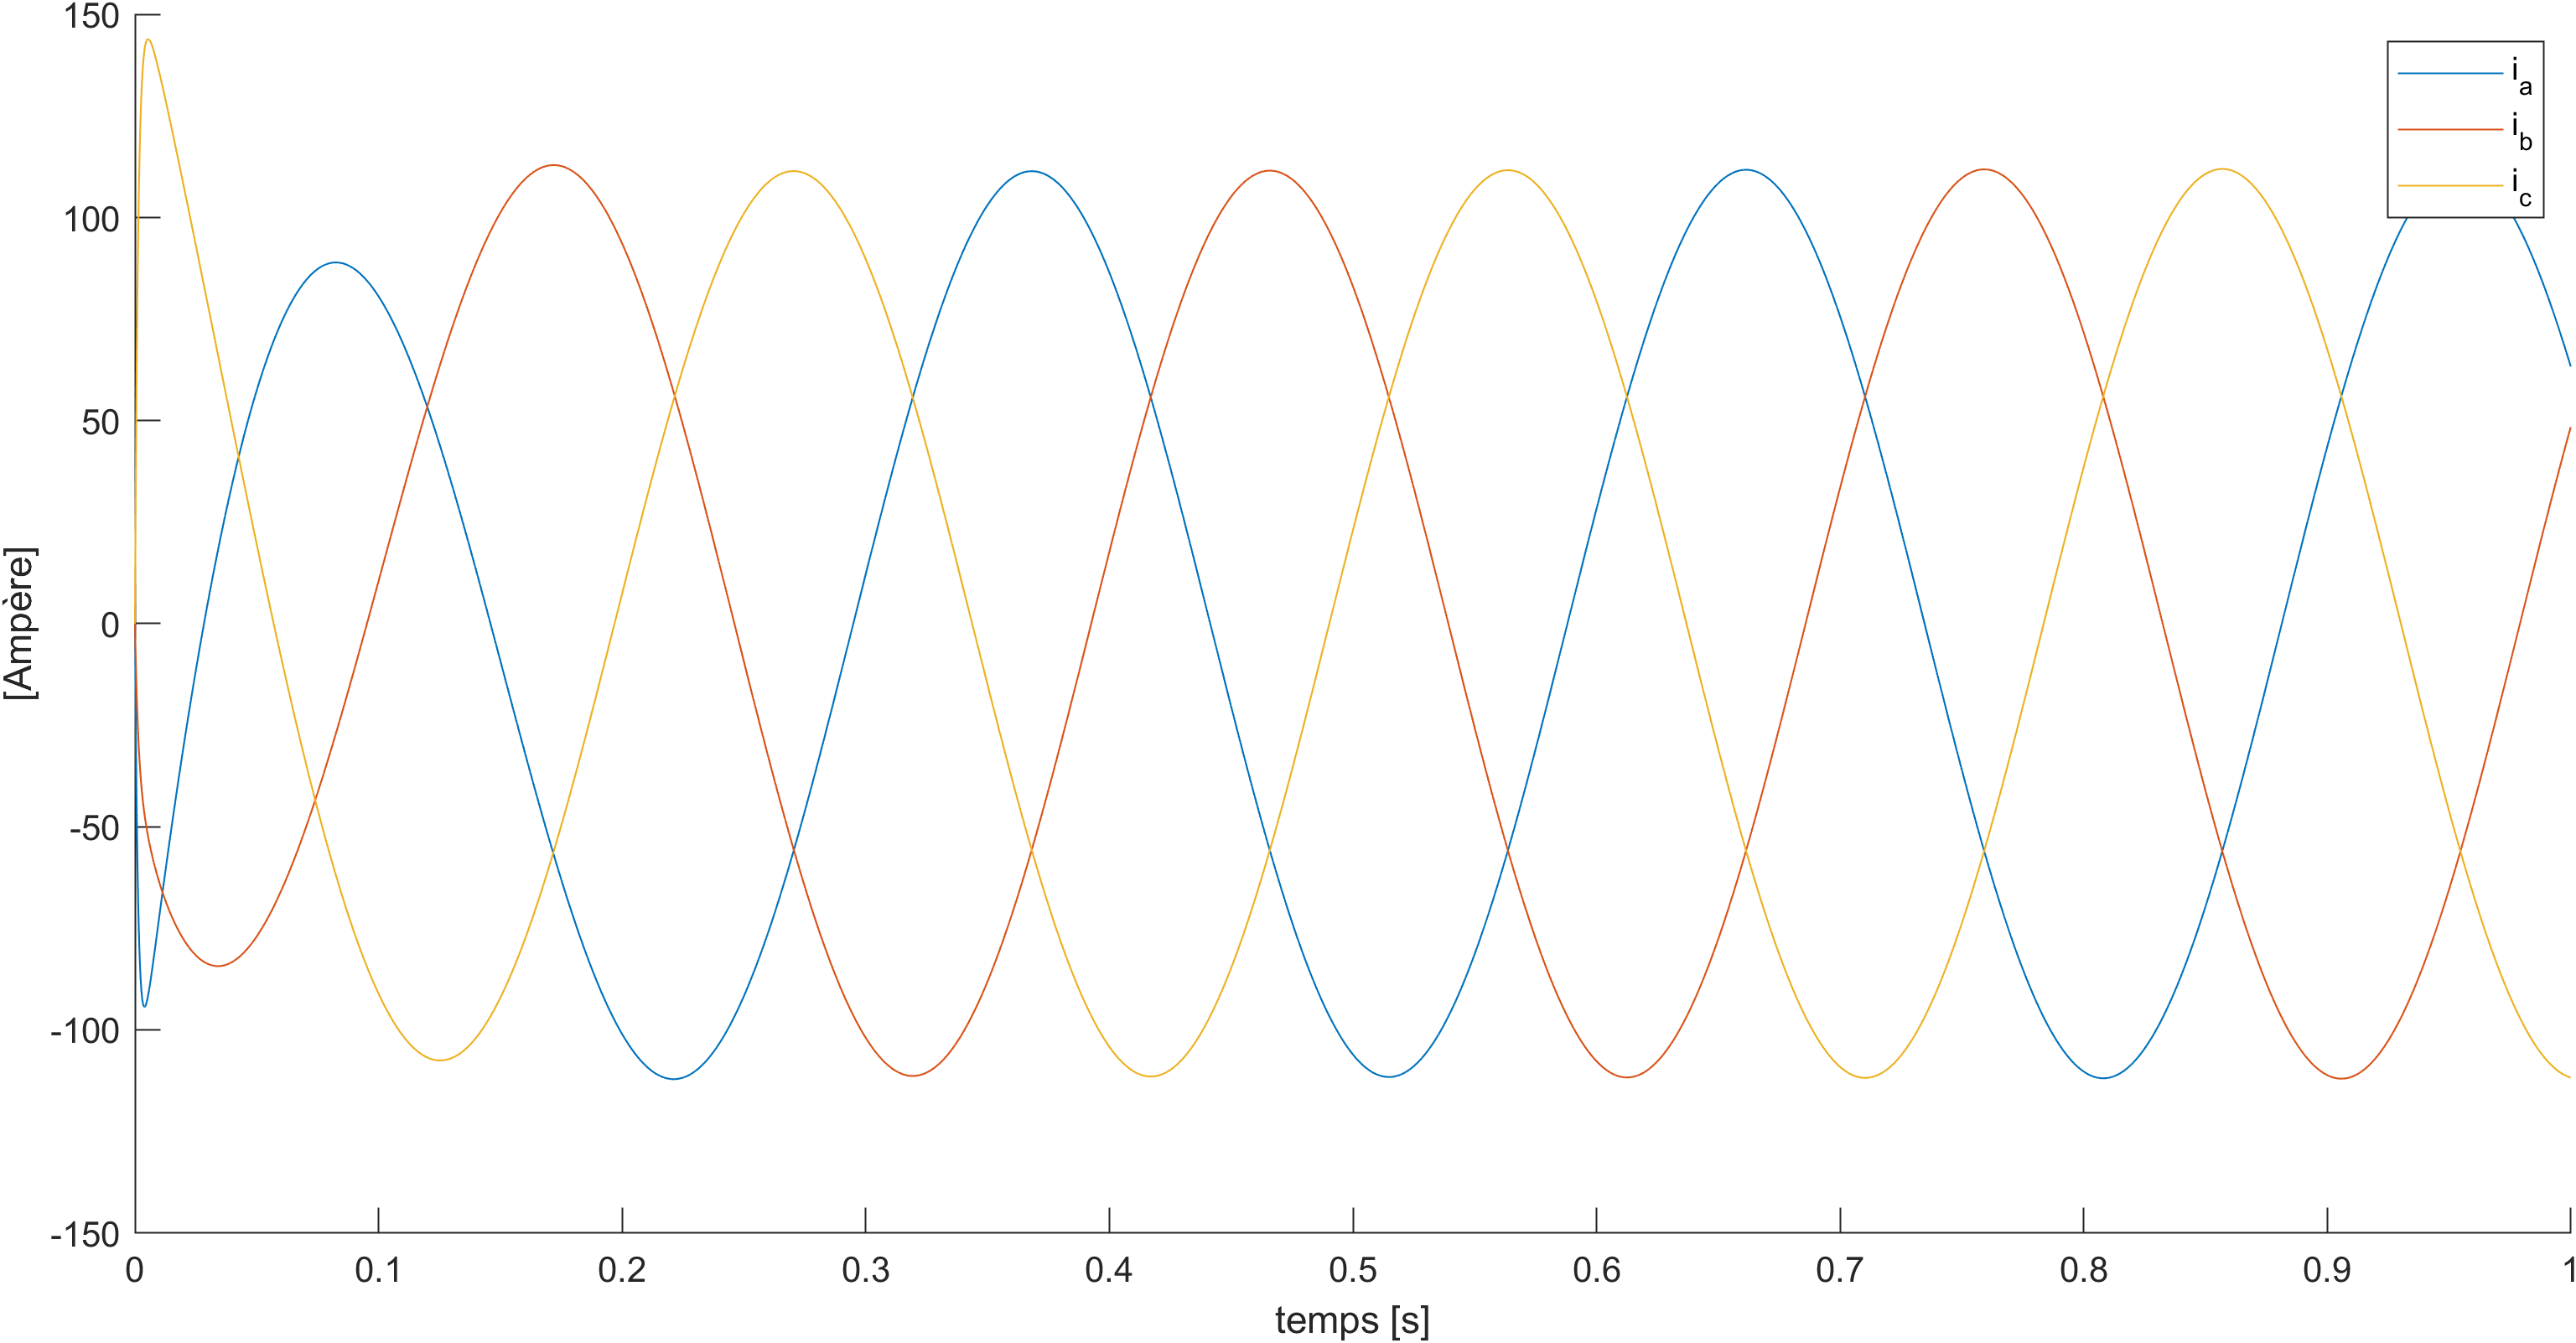
\includegraphics[width=0.8\textwidth]{simusMATLAB/MAS/ir_abc.png} 
    \caption{Courants triphasées du rotor de la MAS mesurées au cours du temps.}
    \label{img-simuMatlab-ir_abc}
\end{figure}

\begin{figure}[!h]
    \centering
    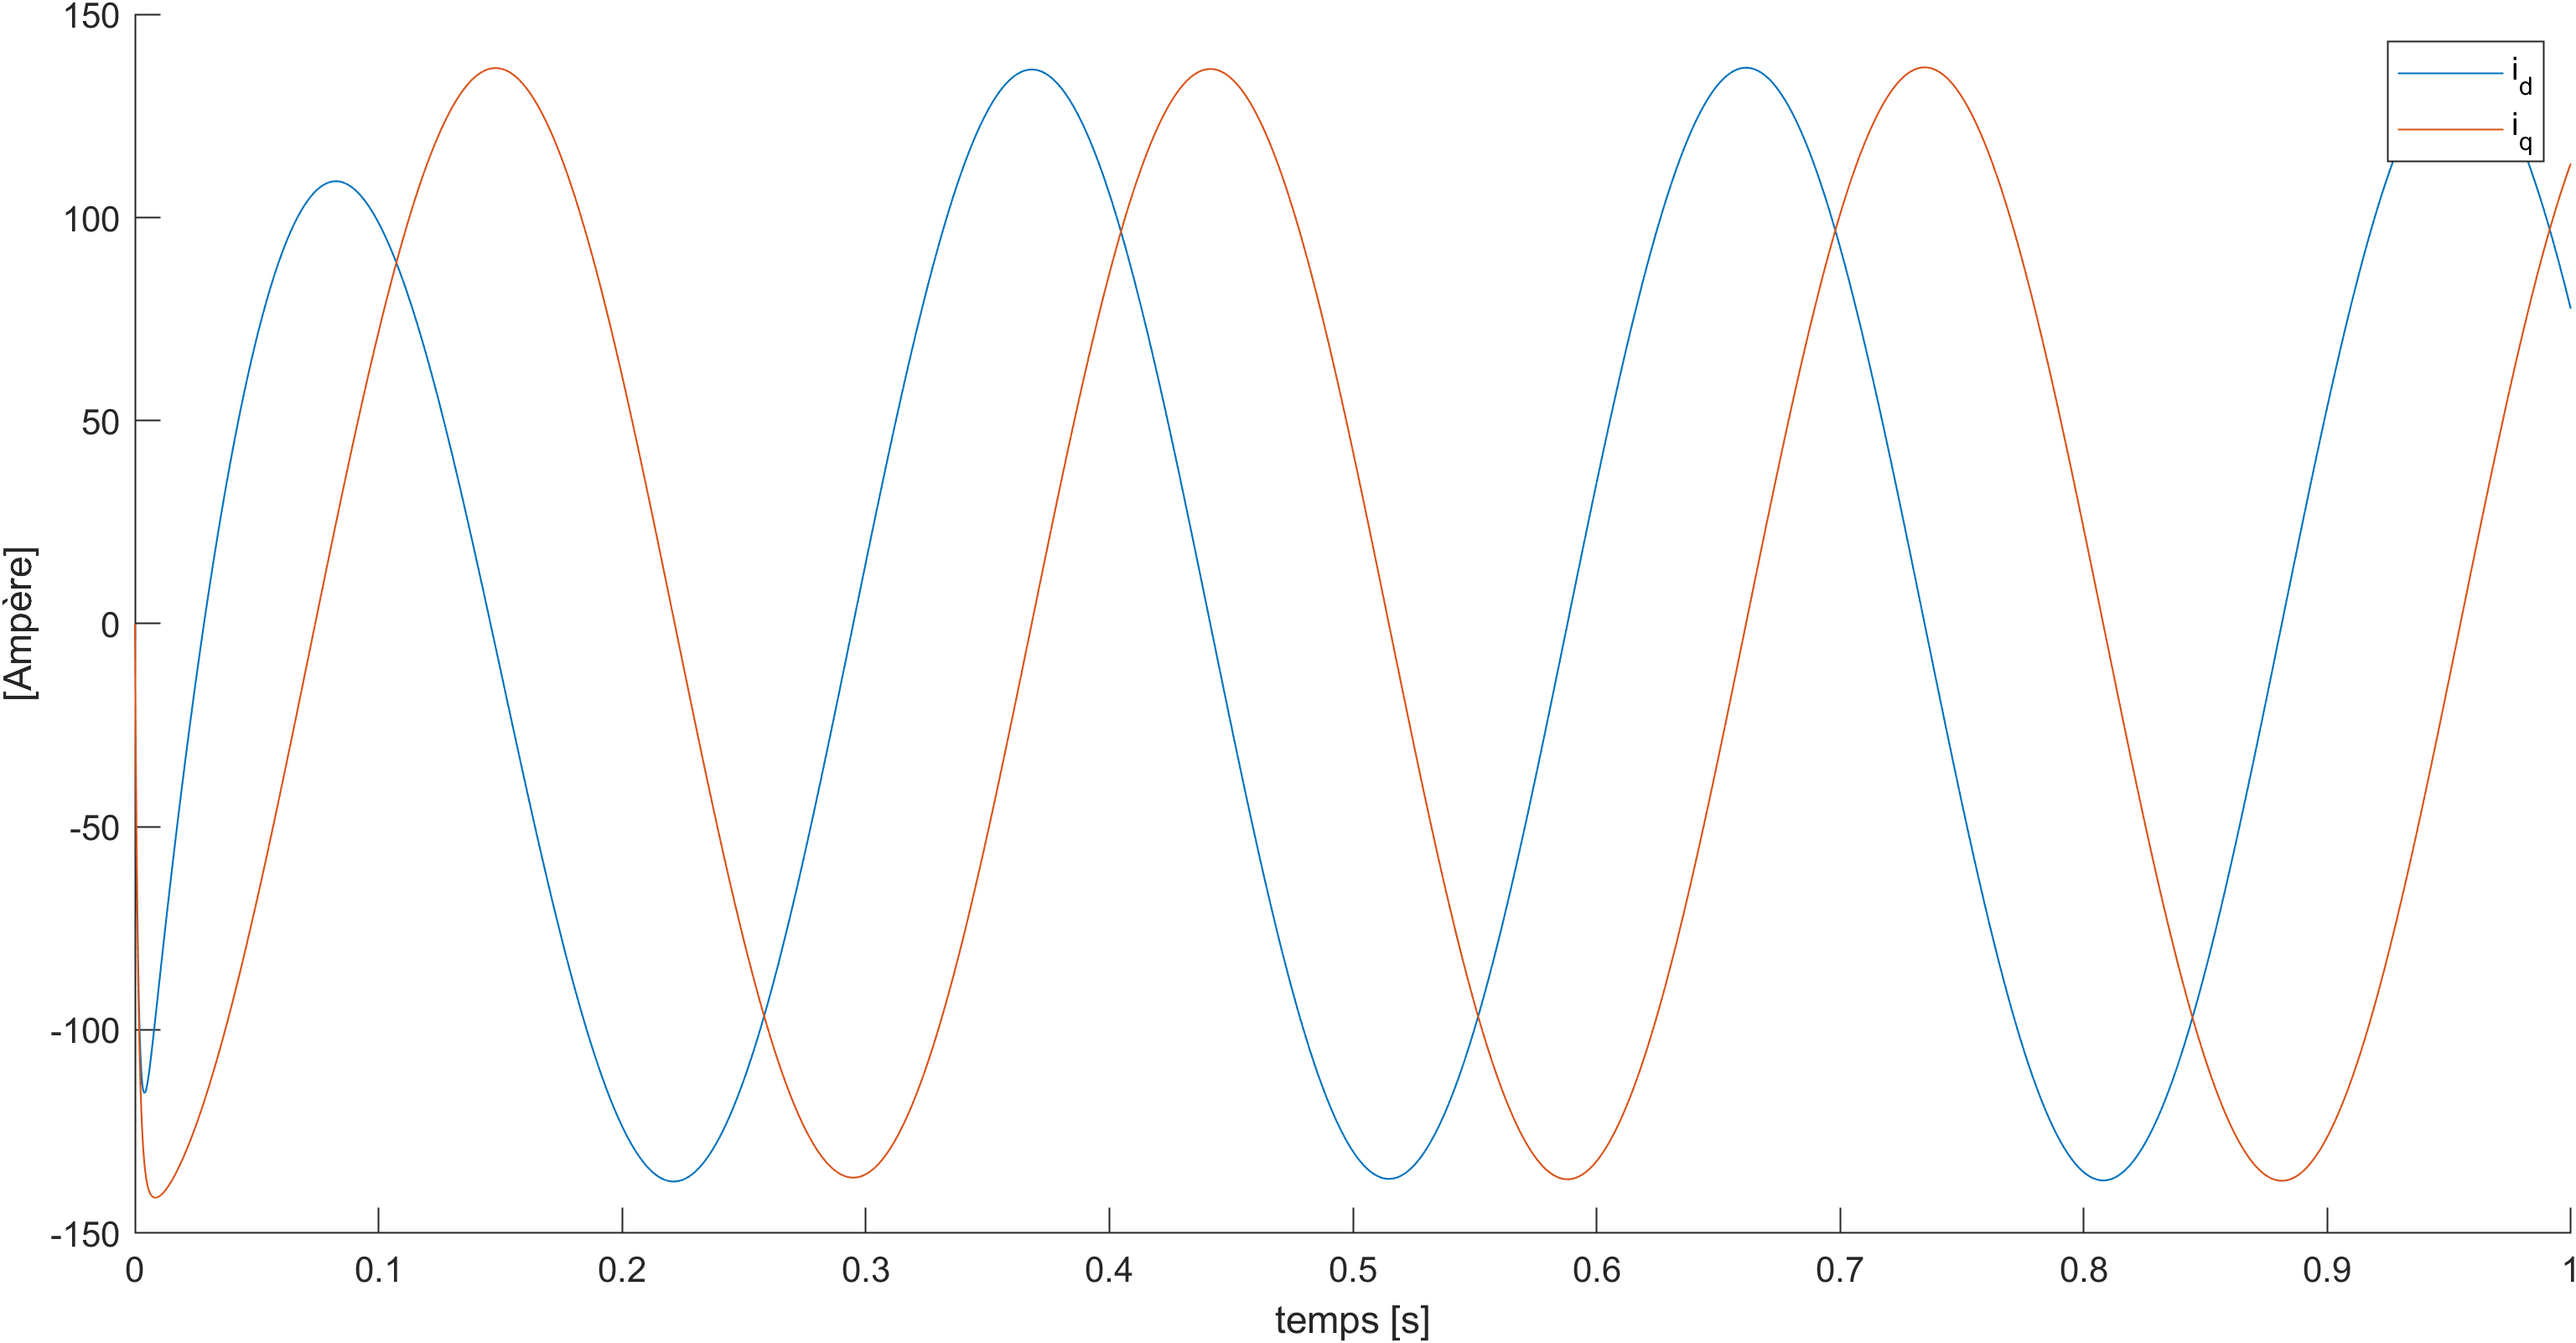
\includegraphics[width=0.8\textwidth]{simusMATLAB/MAS/ir_dq.png} 
    \caption{Courants dans le repère dq du rotor de la MAS au cous du temps.}
    \label{img-simuMatlab-ir_dq}
\end{figure}


Au-delà des mesures de tension et de courant, l'analyse de la courbe de couple de la machine (Figure \ref{img-simuMatlab-Ce}) offre un aperçu de la force de rotation disponible, depuis le démarrage jusqu'à la stabilisation de la vitesse. Cette courbe est indispensable pour évaluer la capacité de la machine à monter en vitesse rapidement et son comportement face aux démarrages fréquents, offrant ainsi une compréhension de ses performances et de sa réactivité.


\begin{figure}[!h]
    \centering
    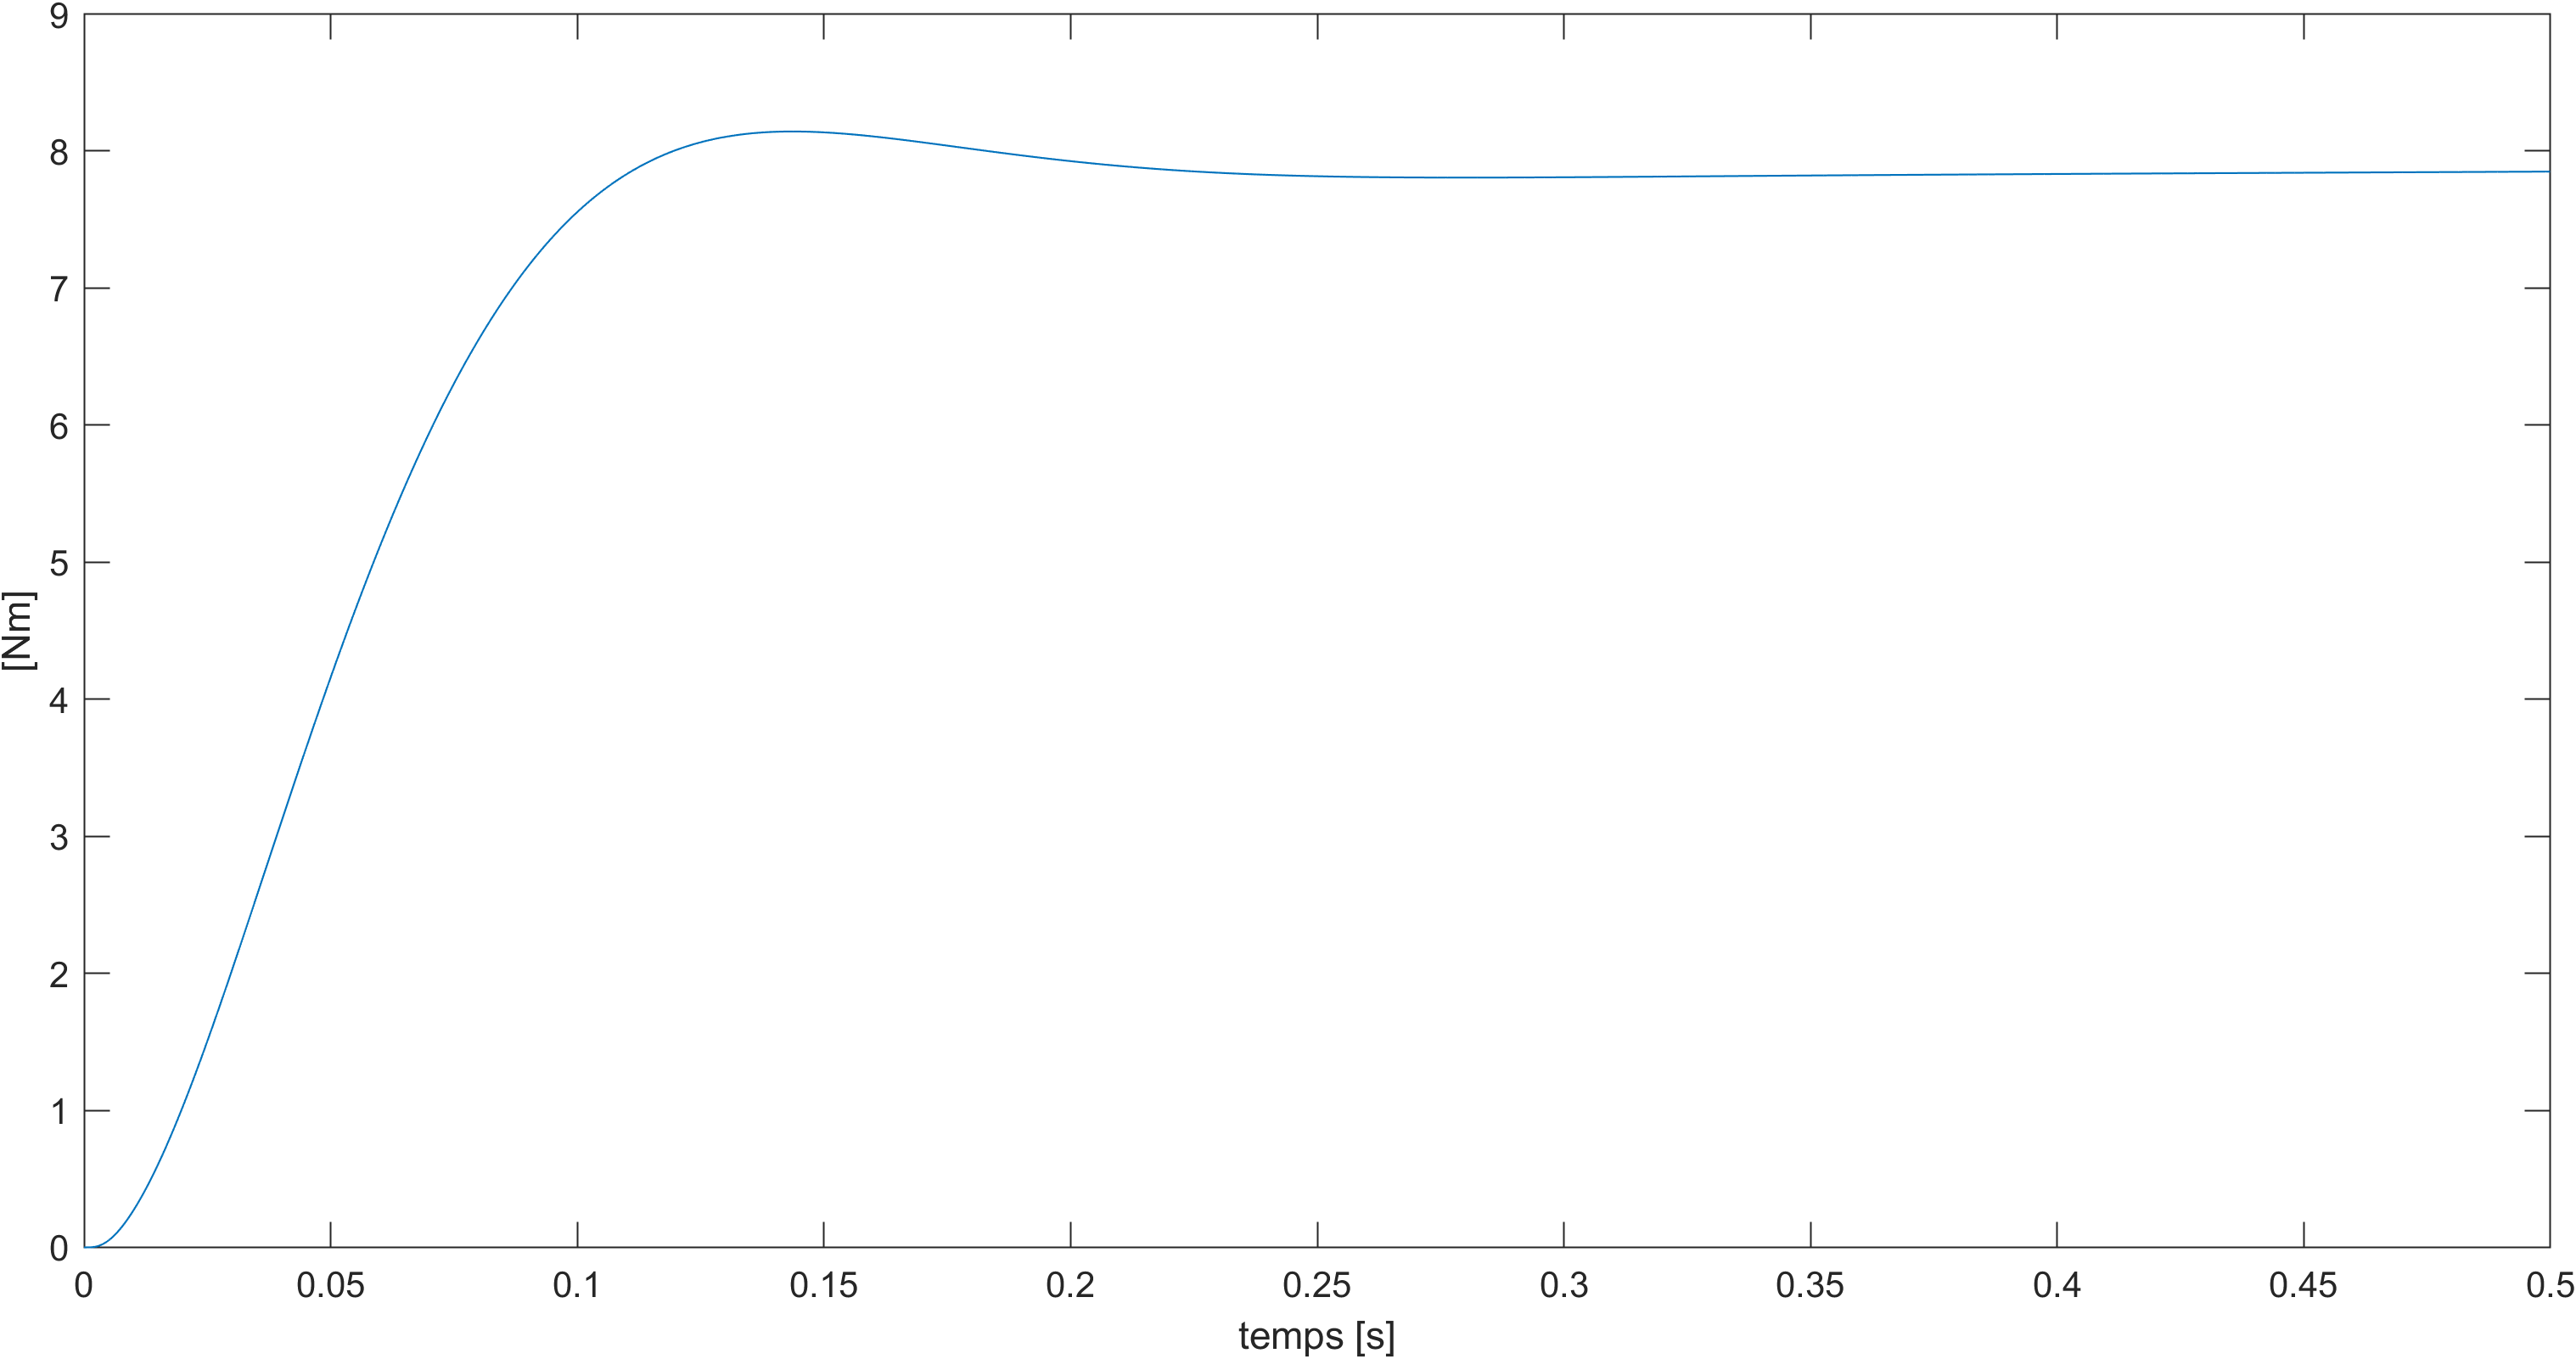
\includegraphics[width=0.8\textwidth]{simusMATLAB/MAS/Ce.png} 
    \caption{Couple de la MAS mesurée au cous du temps.}
    \label{img-simuMatlab-Ce}
\end{figure}

D'autres grandeurs qui ont été mesurées, sont la puissance, flux et torque de la machine, dans les Figures \ref{img-simuMatlab-P}, \ref{img-simuMatlab-phi_r} et \ref{img-simuMatlab-torque} respectivement. C'est possible de voir comme le flux induit dans le rotor de la machine augmente dans un intervalle très court de temps, dans la Figure \ref{img-simuMatlab-phi_r}.


\begin{figure}[!h]
    \centering
    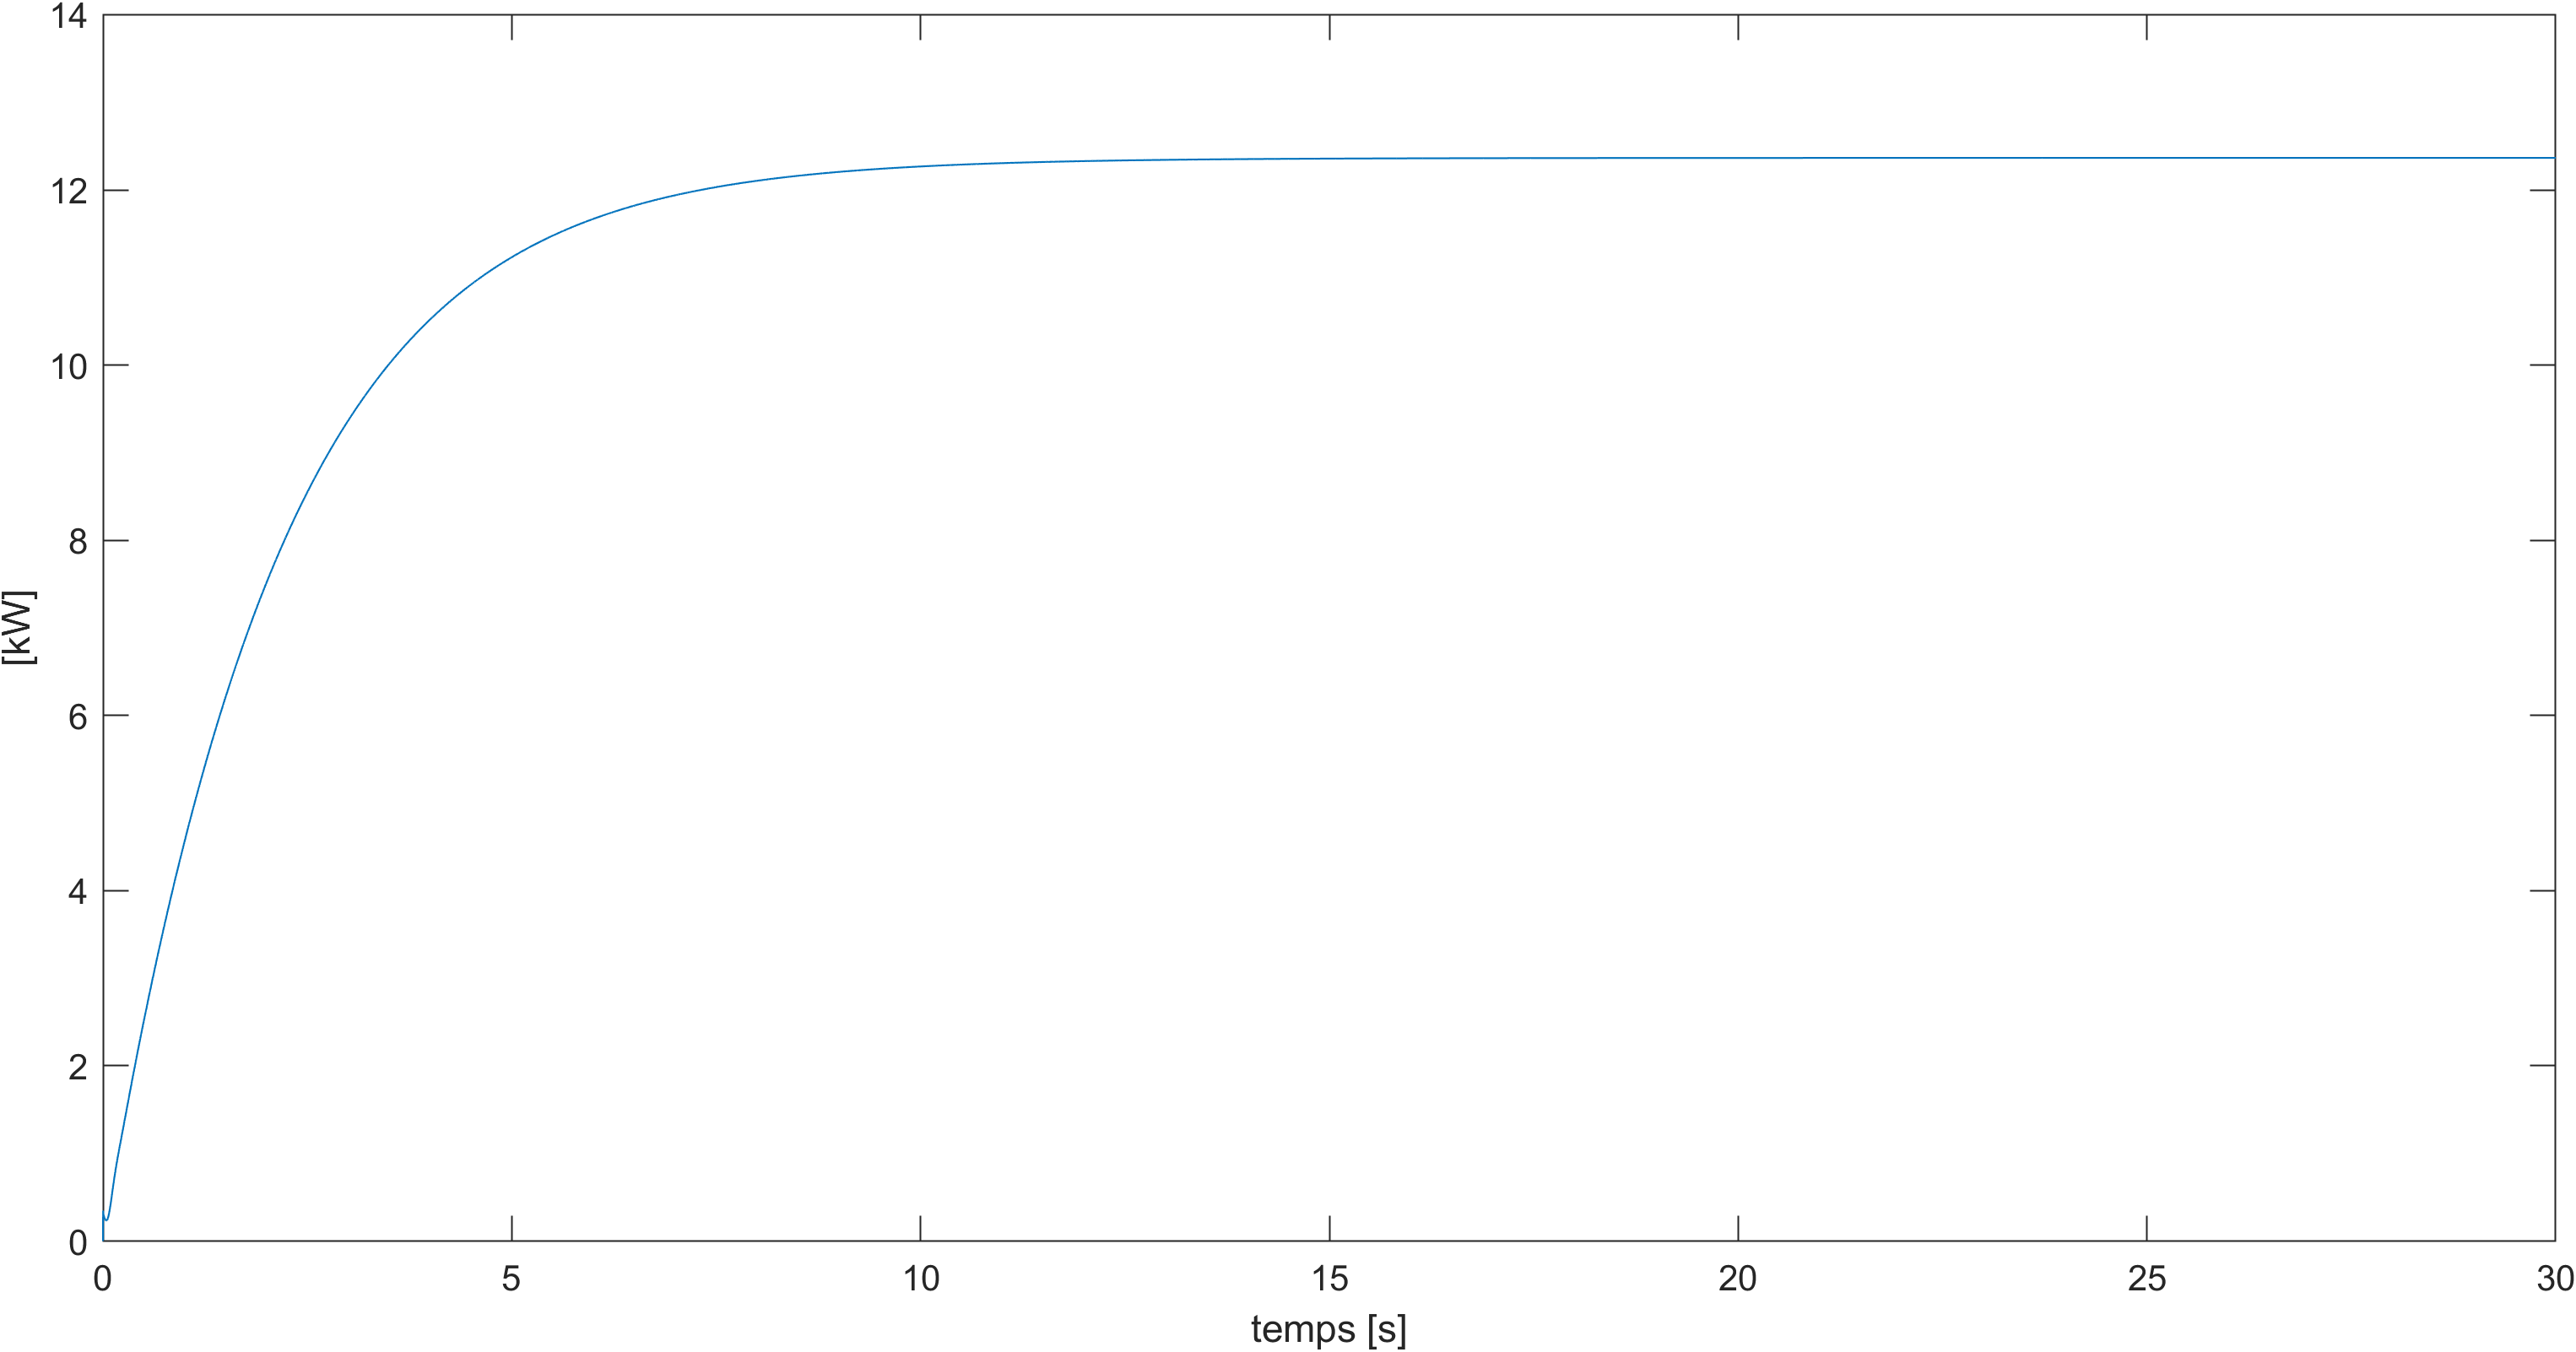
\includegraphics[width=0.8\textwidth]{simusMATLAB/MAS/P.png} 
    \caption{Puissance de la MAS mesurée au cous du temps.}
    \label{img-simuMatlab-P}
\end{figure}




\begin{figure}[!h]
    \centering
    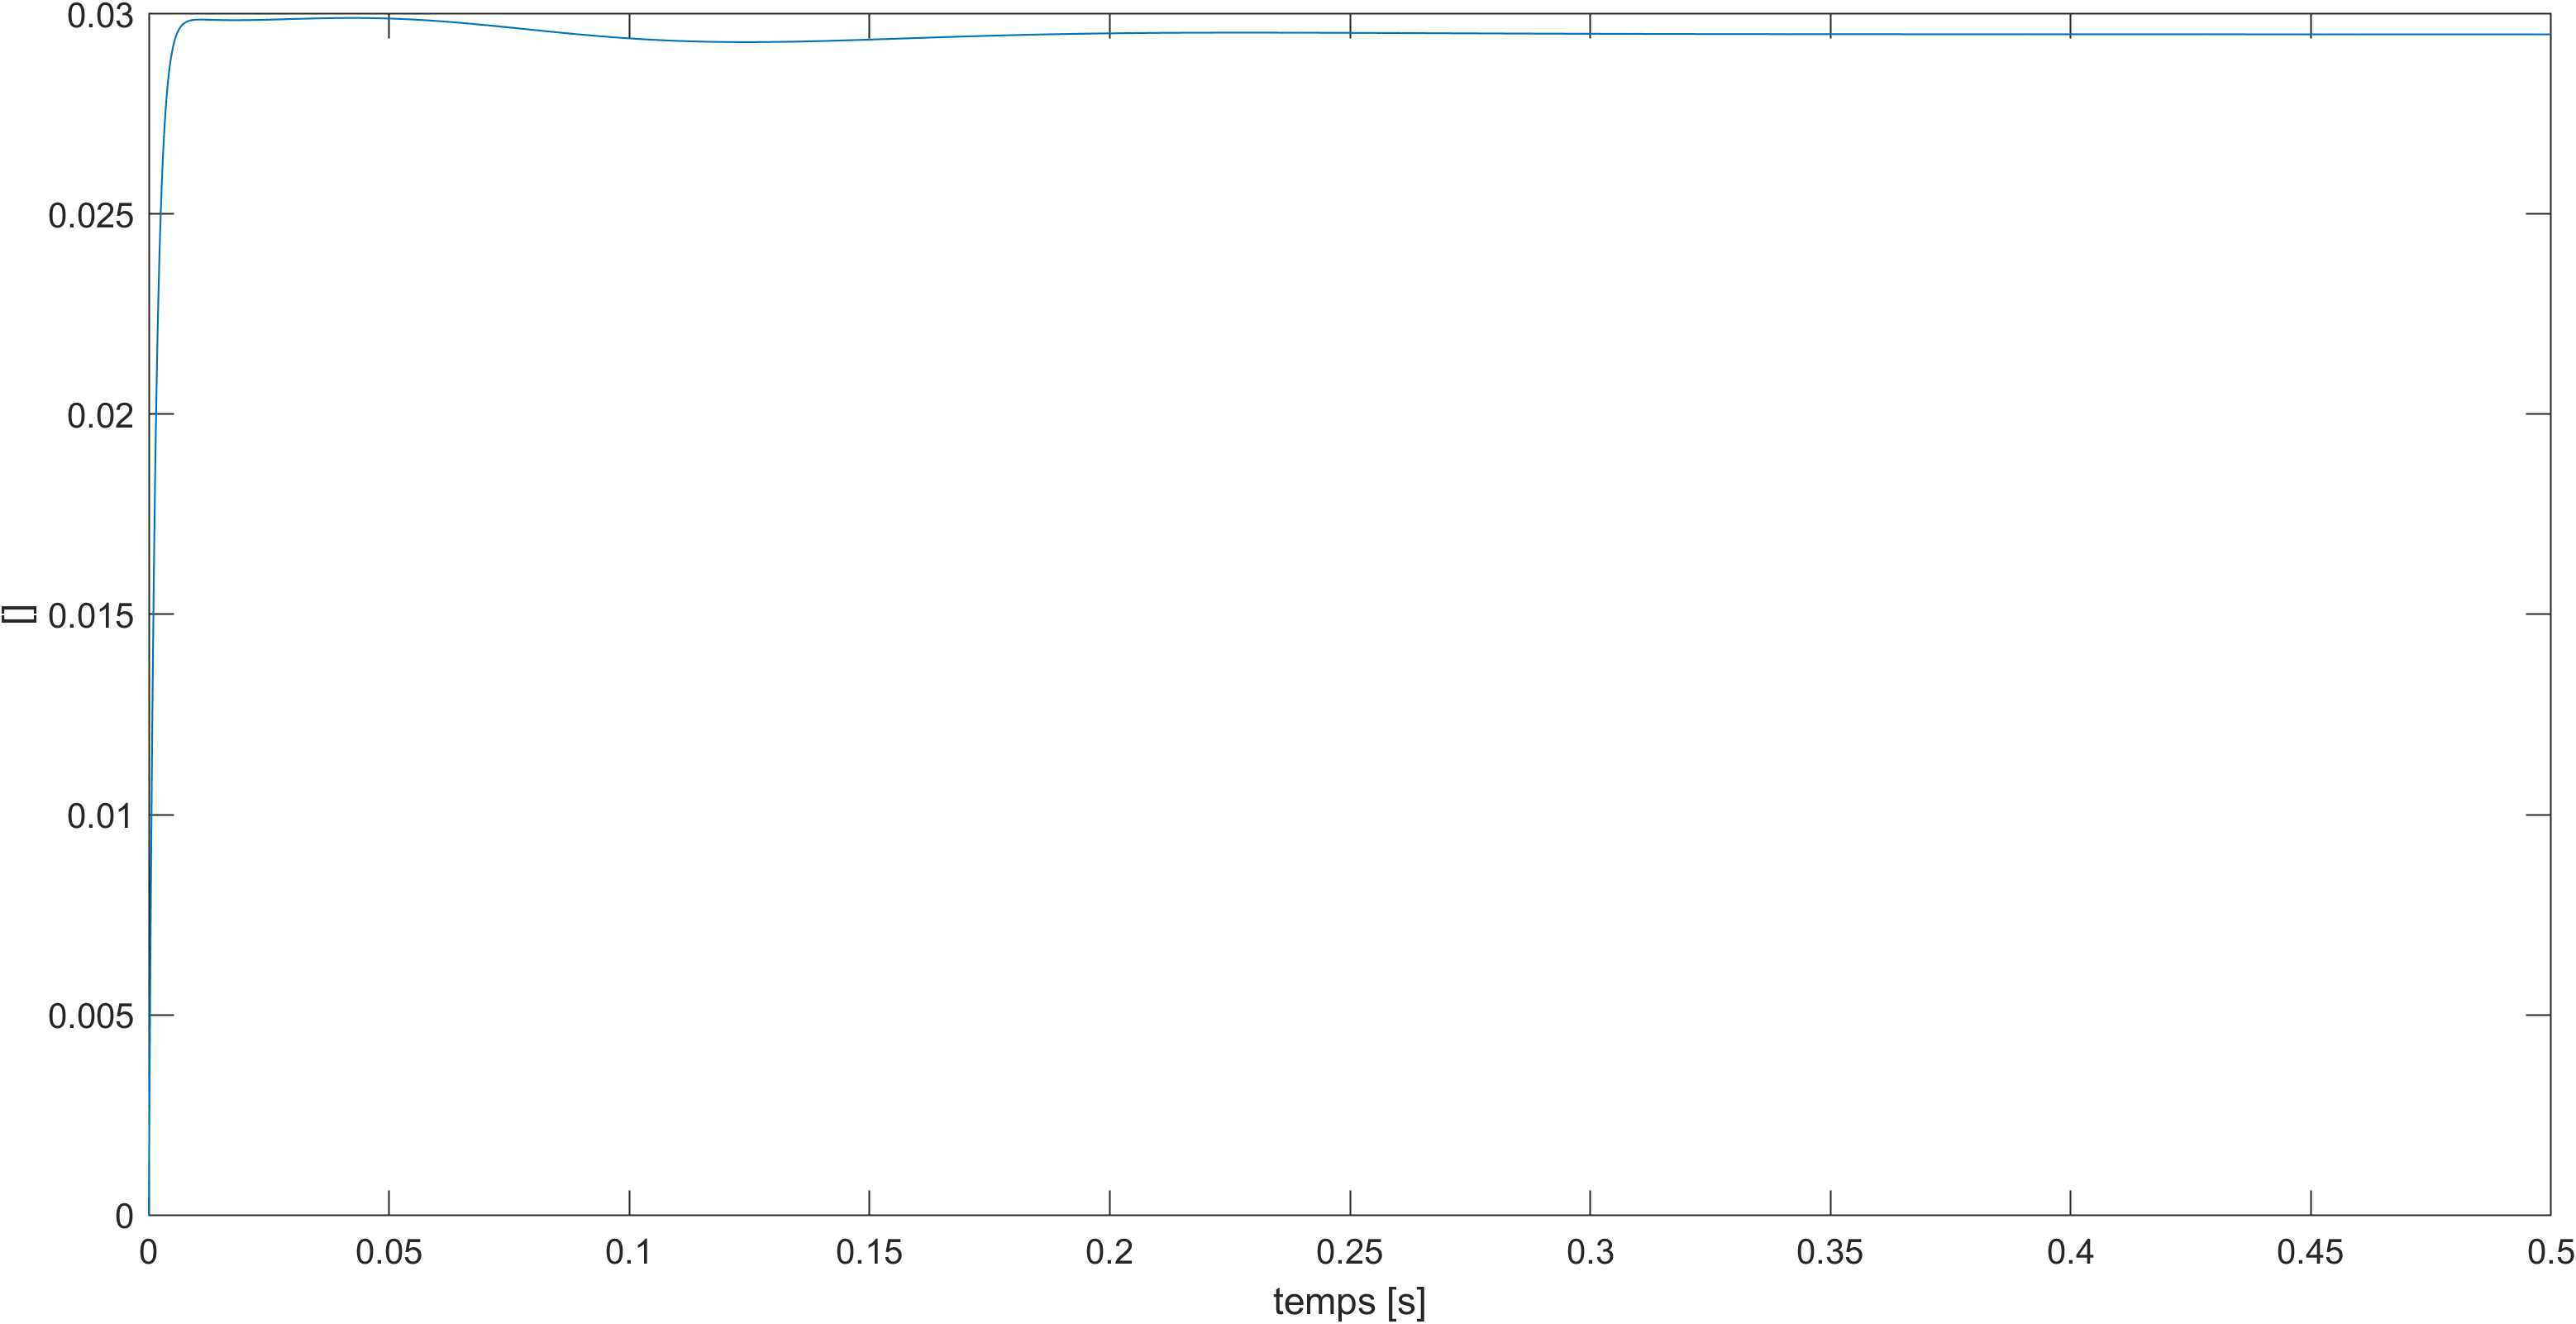
\includegraphics[width=0.8\textwidth]{simusMATLAB/MAS/phi_r.png} 
    \caption{Flux dans le rotor de la MAS mesurée au cous du temps.}
    \label{img-simuMatlab-phi_r}
\end{figure}



\begin{figure}[!h]
    \centering
    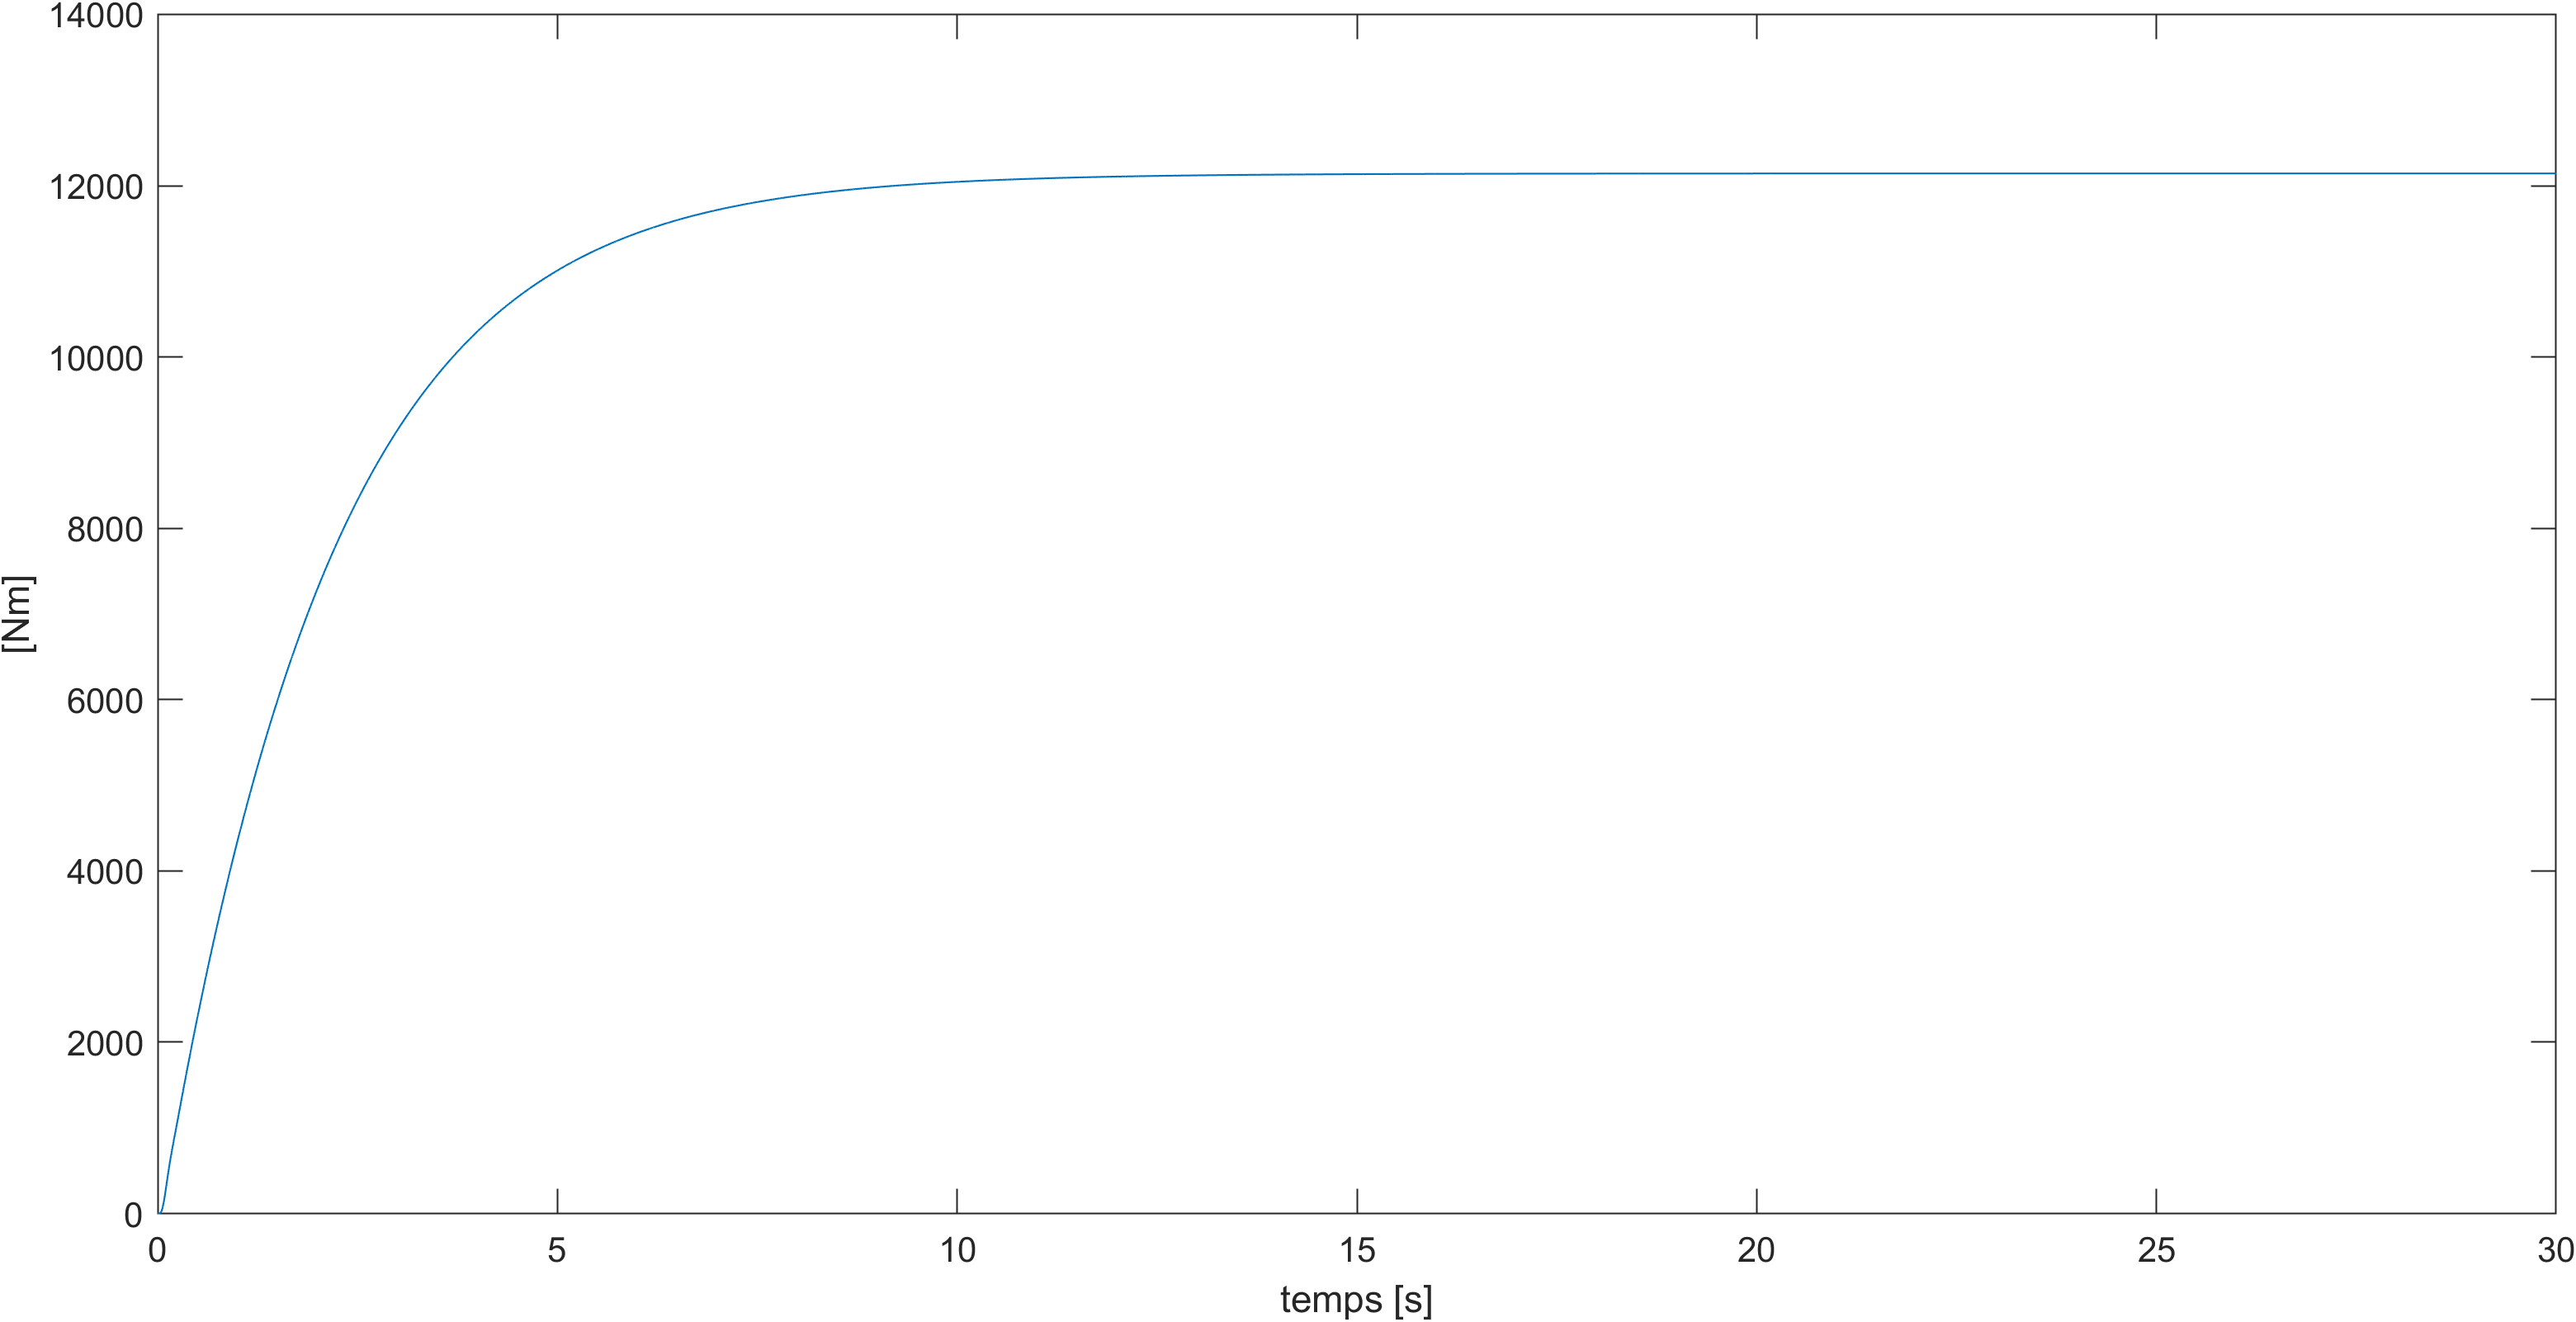
\includegraphics[width=0.8\textwidth]{simusMATLAB/MAS/torque.png} 
    \caption{Torque de la MAS mesurée au cours du temps.}
    \label{img-simuMatlab-torque}
\end{figure}

Afin de vérifier que le système est cohérent dans le régime permanent, deux autres relations du modèle ont été vérifiées, comme le montre le diagramme de la Figure \ref{img-CI_verifier_relations}. Les figures \ref{img-simuMatlab-comparation_wm} et \ref{img-simuMatlab-relation} montrent que le système converge dans le régime permanent. 

\begin{figure}[!h]
    \centering
    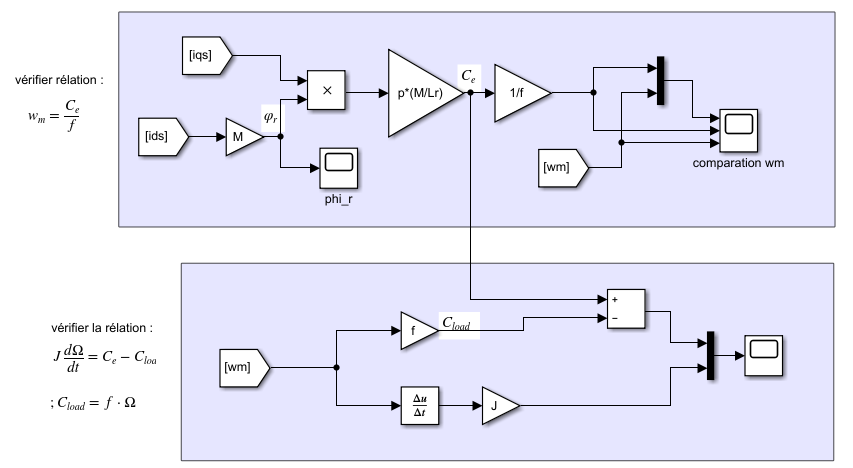
\includegraphics[width=0.9\textwidth]{imgsMATLAB/MAS/CI/CI_verifier_relations.png} 
    \caption{Schémas de validation du modèle de la MAS.}
    \label{img-CI_verifier_relations}
\end{figure}



\begin{figure}[!h]
    \centering
    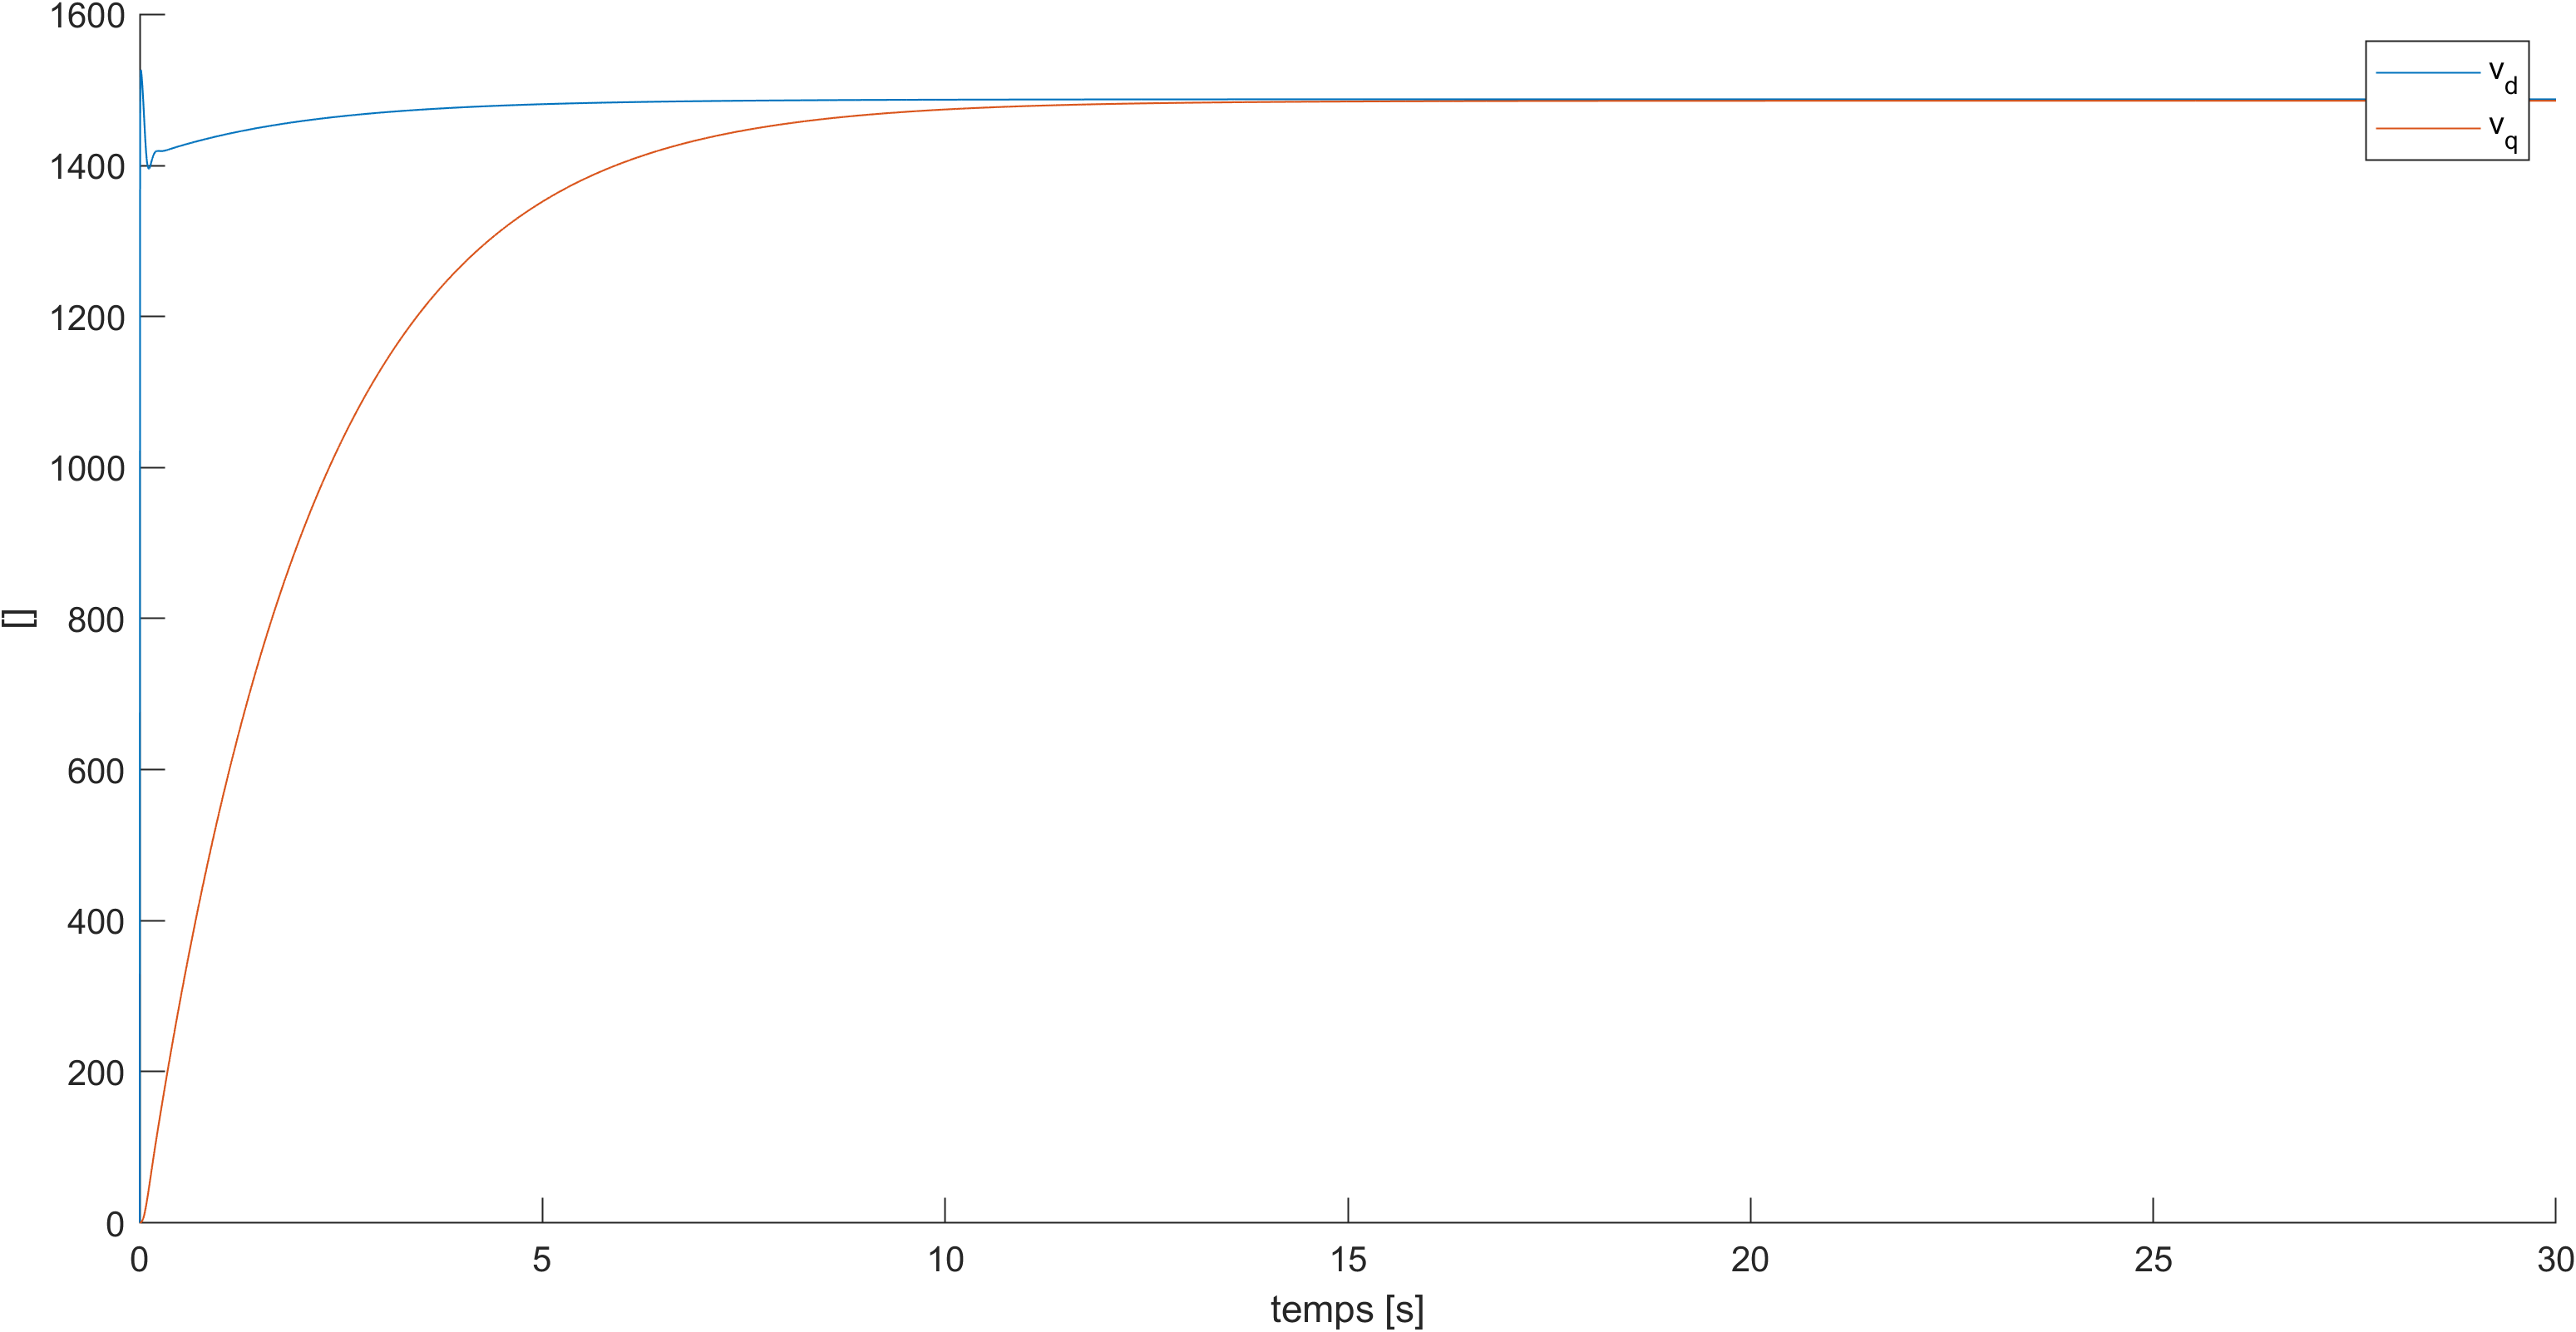
\includegraphics[width=0.8\textwidth]{simusMATLAB/MAS/comparation_wm.png} 
    \caption{Vérification de la évolution de la relation $\omega_m = \frac{C_e}{f}$ de la MAS.}
    \label{img-simuMatlab-comparation_wm}
\end{figure}


\begin{figure}[!h]
    \centering
    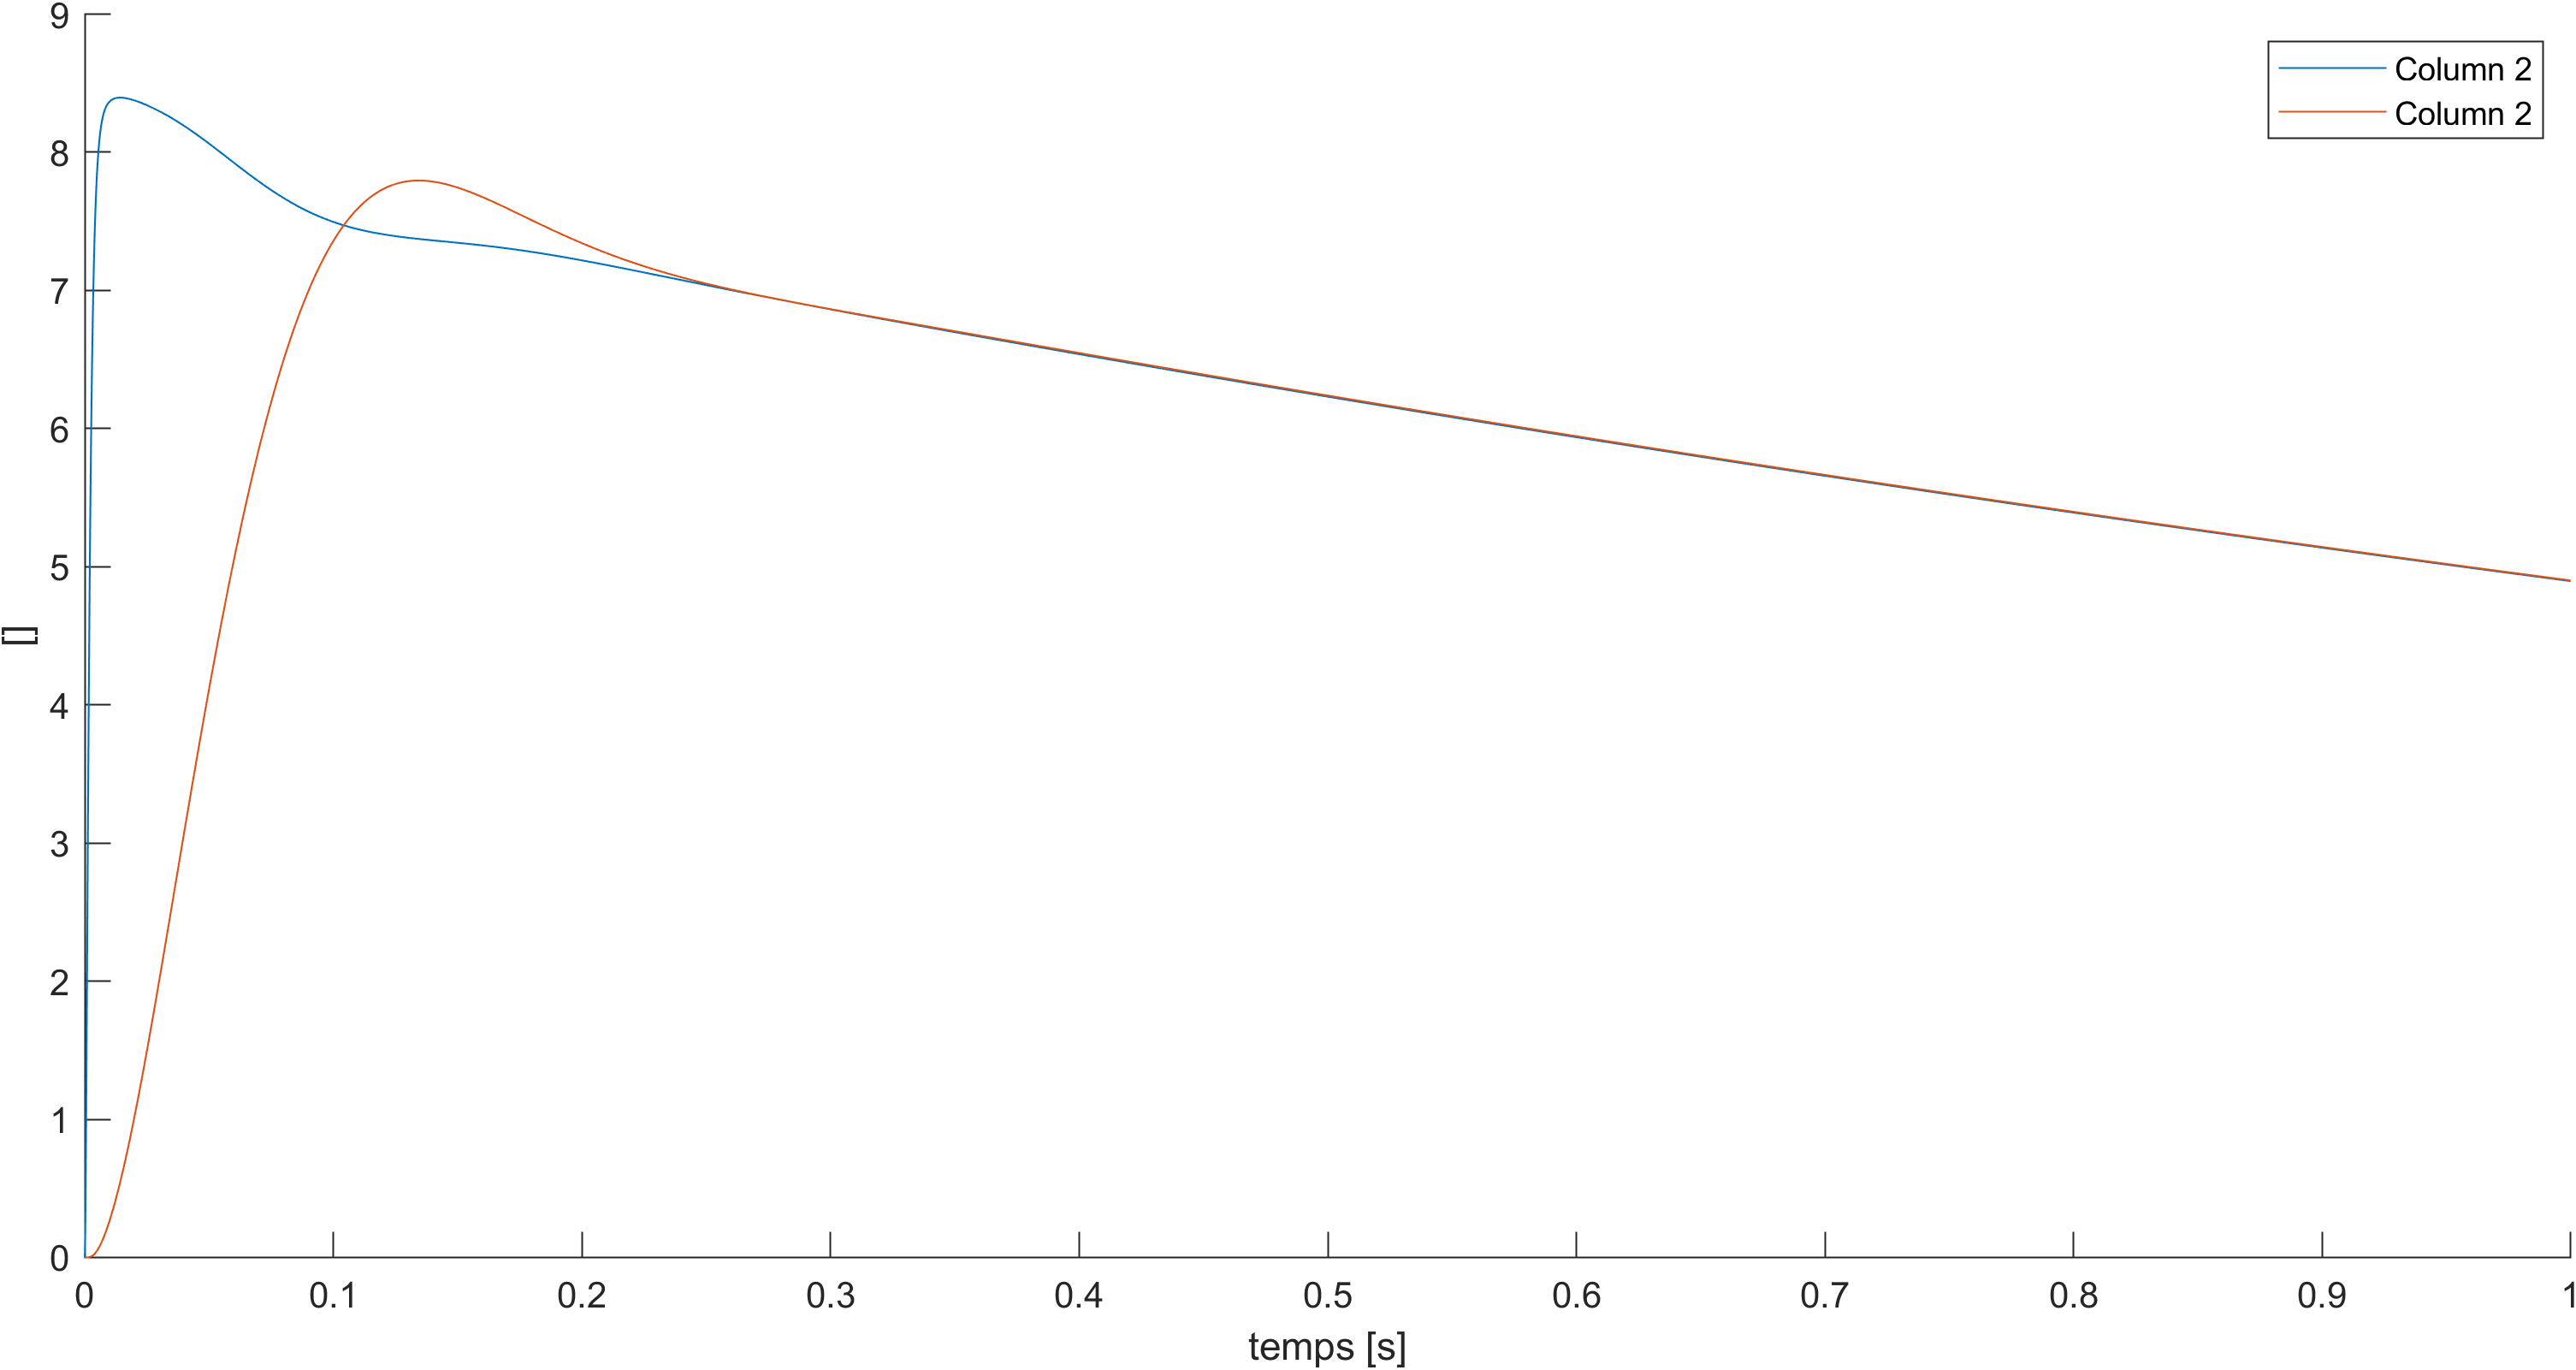
\includegraphics[width=0.8\textwidth]{simusMATLAB/MAS/relation.png} 
    \caption{Vérification de la évolution de la relation \ref{eq:dWm} de la MAS.}
    \label{img-simuMatlab-relation}
\end{figure}


%---------------------------------------
\FloatBarrier
\subsection{Simulation MADA}
%---------------------------------------

Afin de valider le modèle de la machine asynchrone de double alimentation les paramètres suivantes ont étés adoptés : $p = 2; R_s = 60 \cdot m\Omega; R_r = 38 m\Omega; L_s = L_{fs} + L_m, L_r = L_{fr} + L_m, \text{avec} L_m=12mH, L_{fr} = 180uH, \text{et} L_{fs}= 360uH; M_{sr} = L_m; f = -22 kg \cdot m^2 \cdot s^-1; J = 0.4 kg \cdot m^2$. Ces paramètres utilisées cherchent simuler une MADA qui opère comme génératrice éolienne. Dans cette machine simulée, au contraire de la MAS simulée précédemment, une charge de $5 \cdot 10^3 N\cdot m$ a été connecté, en plus du phénomène de frottement. 

En simulant d'abord la MADA agissant comme une machine asynchrone à induction, avec l'alimentation du rotor nulle, il est possible de vérifier son fonctionnement en observant la courbe de vitesse angulaire du rotor, qui présente un forte comportement oscillatoire dans sa démarrage mais que converge au valeur de $150 rad/s$ (Figure \ref{img-simuMADA-wm}). Pour ce première moment, fonctionnant comme moteur, la valeur de f a été changé à $0.1 kg \cdot m^2$. 


\begin{figure}[!h]
    \centering
    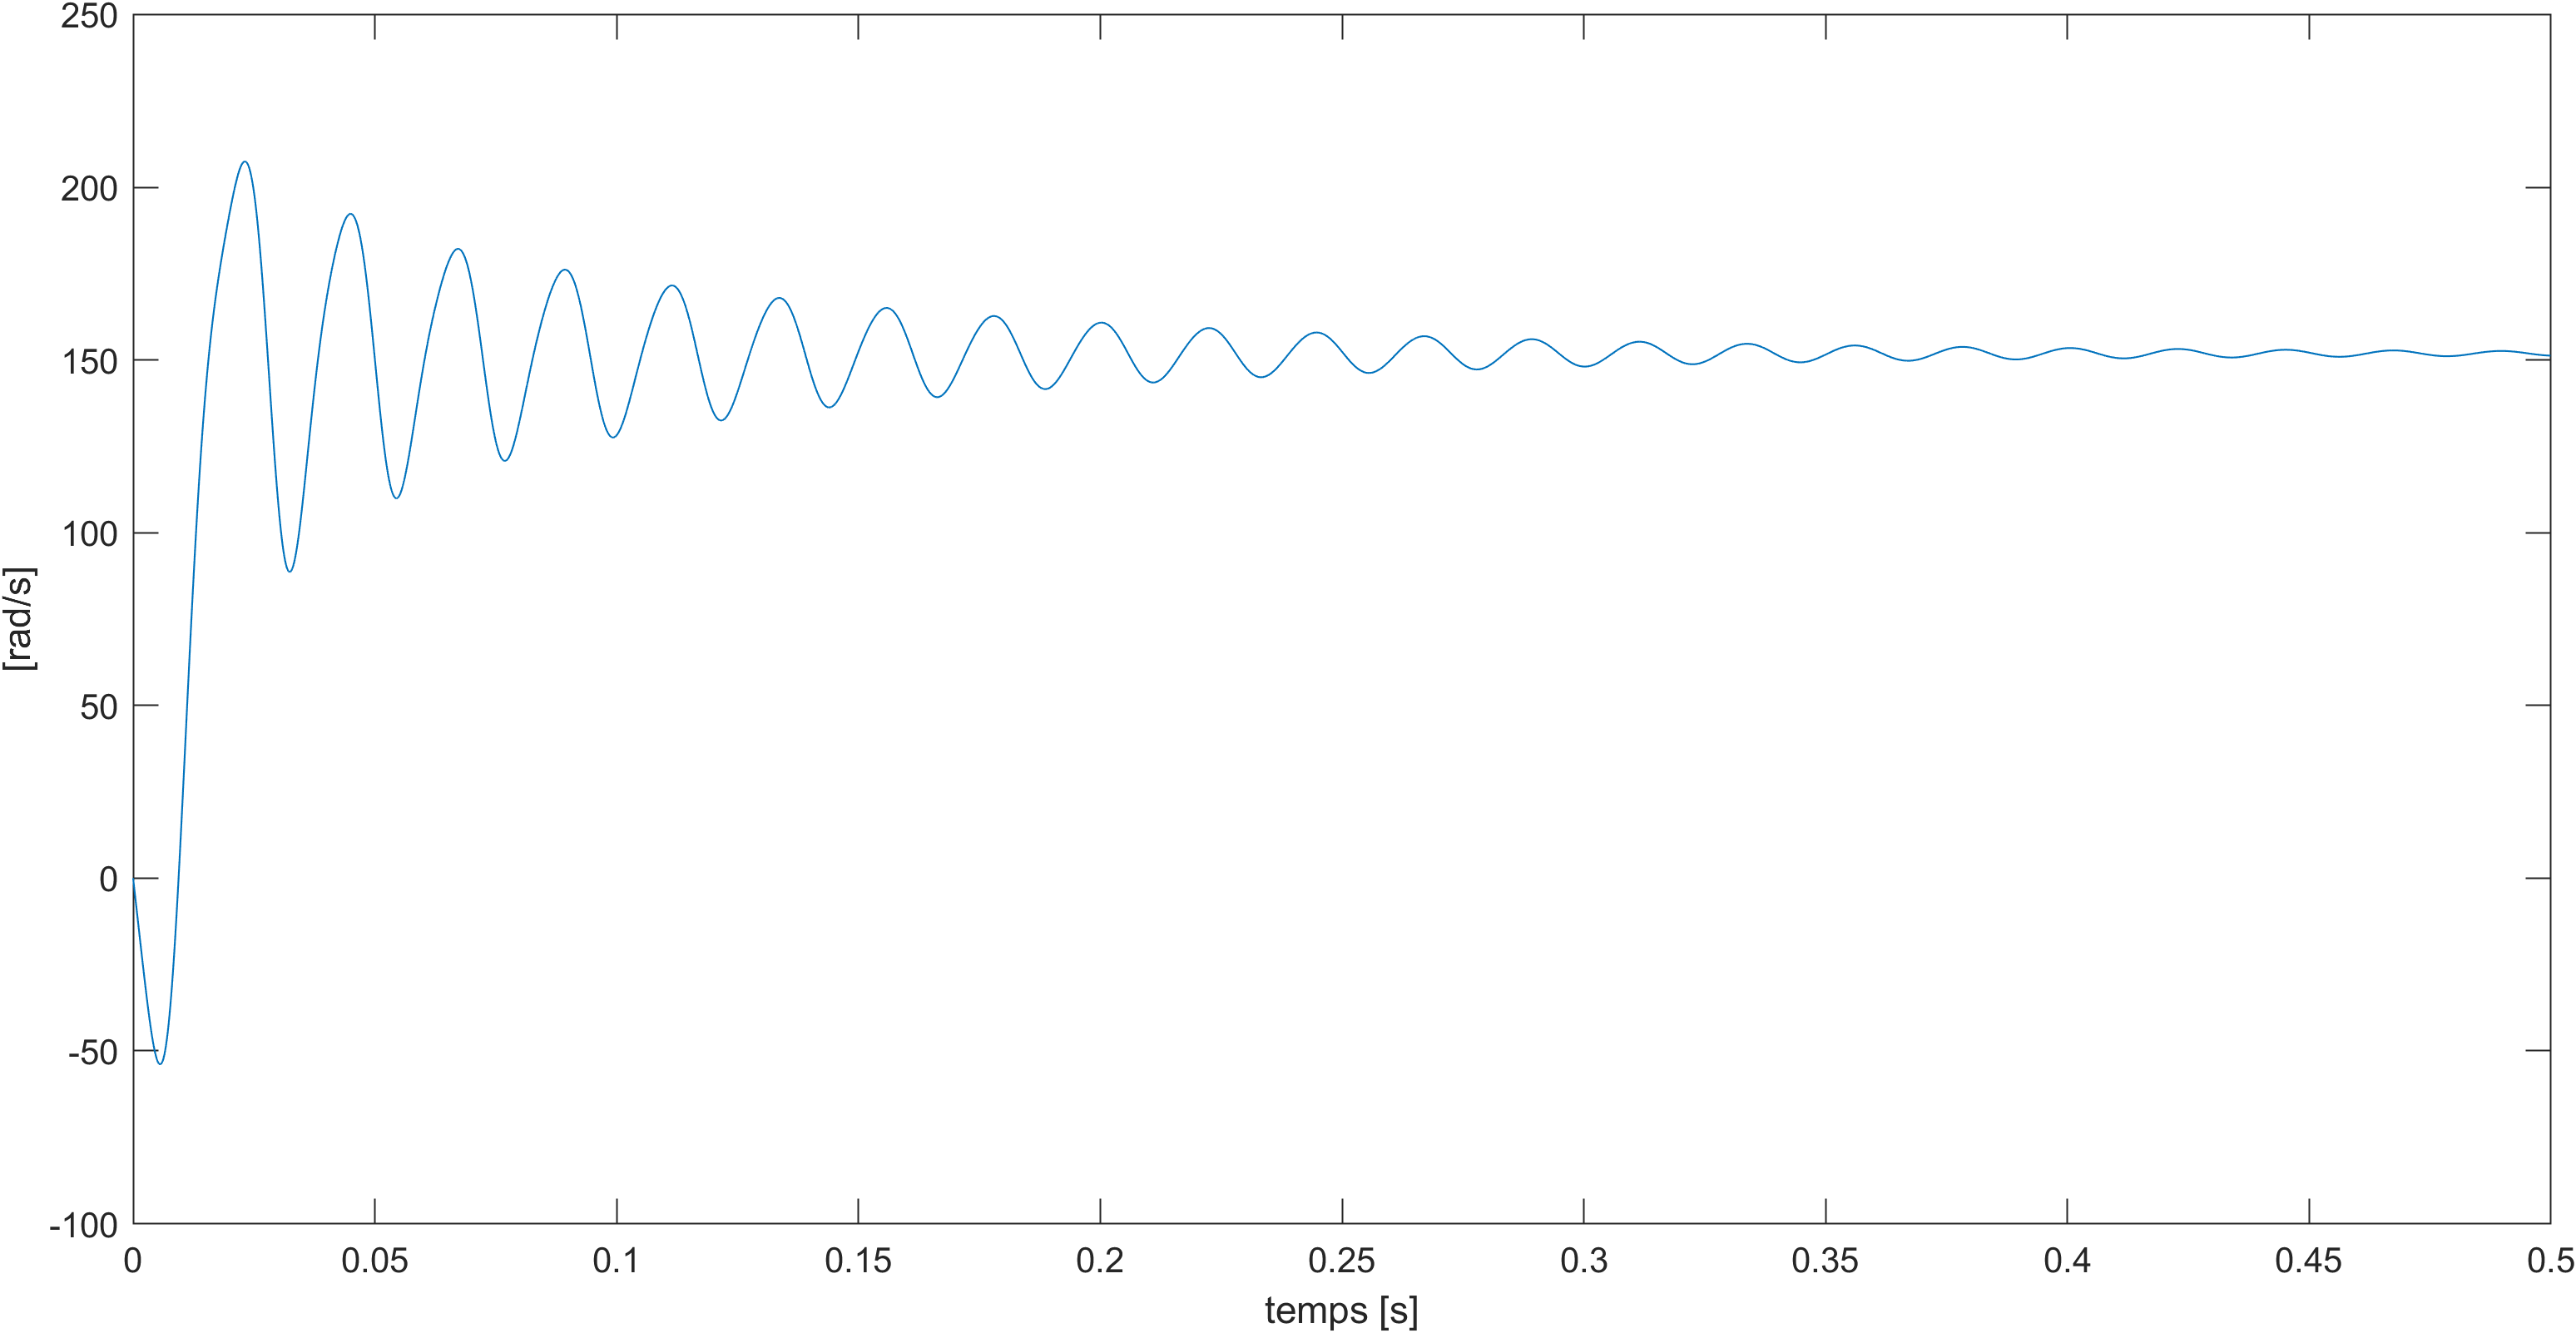
\includegraphics[width=0.8\textwidth]{simusMATLAB/MADA/wm.png} 
    \caption{Vitesse angulaire du rotor de la MADA mesurée au cous du temps.}
    \label{img-simuMADA-wm}
\end{figure}

Il est également possible de vérifier les valeurs de courant et de tension de la machine en cours de fonctionnement. La Figure \ref{img-simuMADA-ir_abc} montre le transitoire des courants triphasés dans le rotor de la machine, puis leur stabilisation en régime permanent. Il en va de même pour les figures \ref{img-simuMADA-ir_alphabeta} et \ref{img-simuMADA-is_abc}, où \ref{img-simuMADA-is_abc} met en évidence les courants triphasés transitoires dans le stator de la machine. 


\begin{figure}[!h]
    \centering
    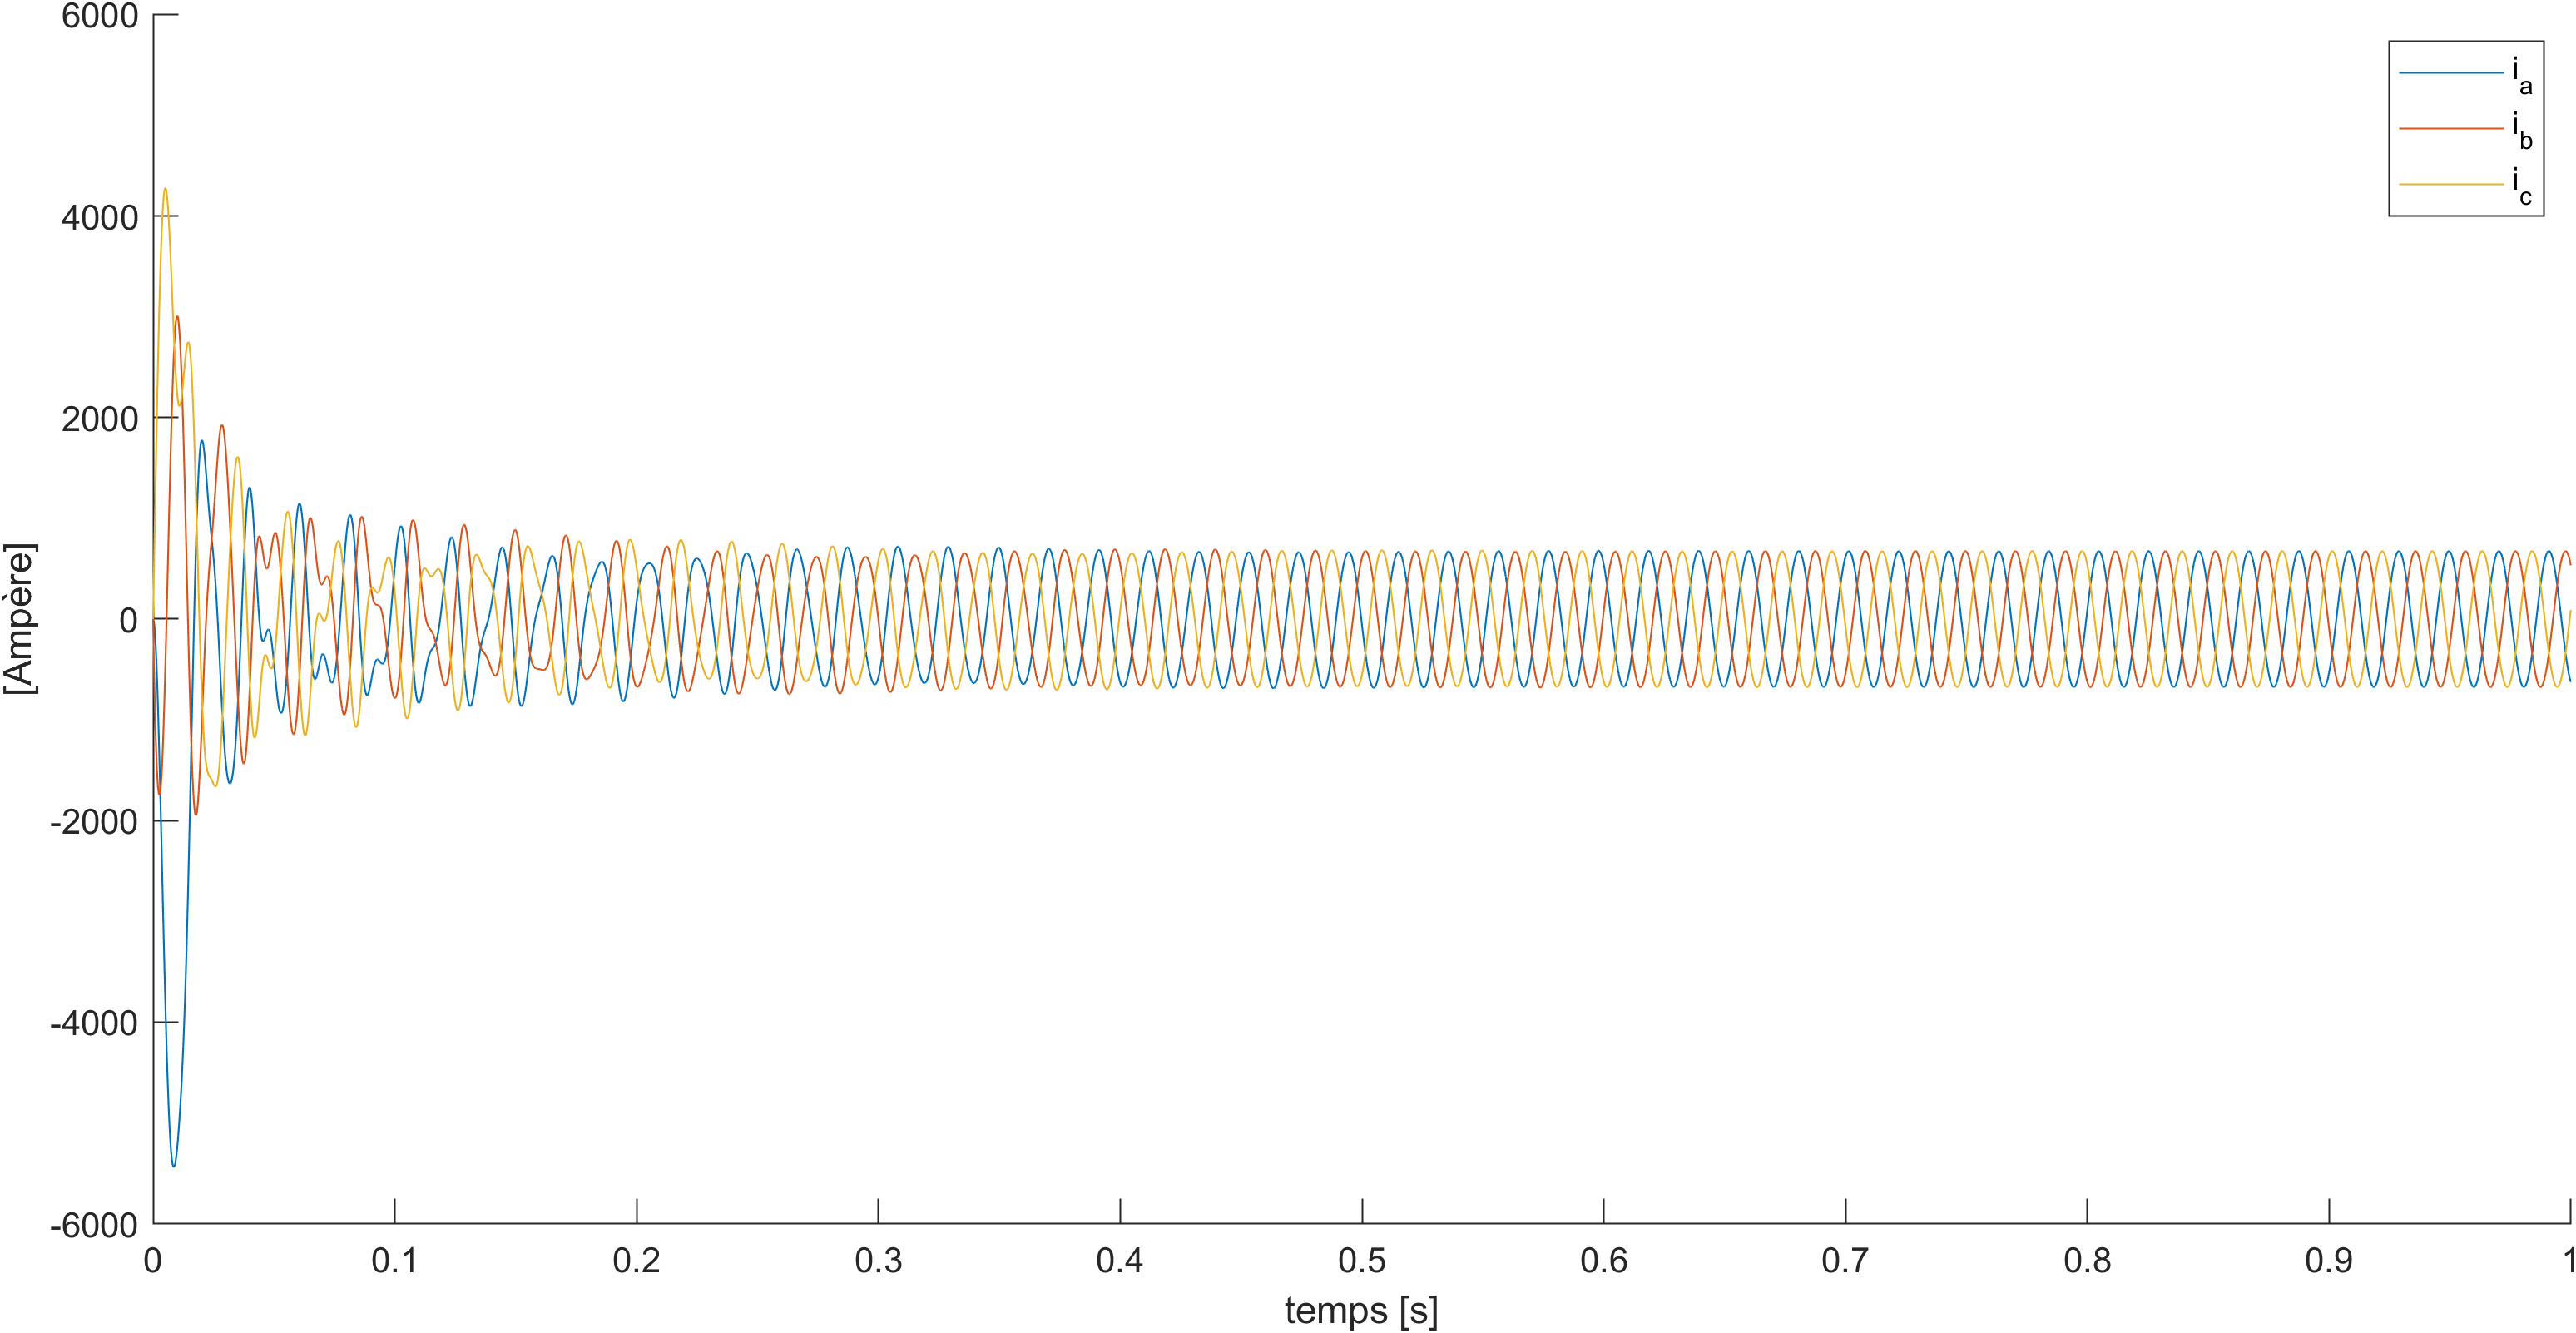
\includegraphics[width=0.8\textwidth]{simusMATLAB/MADA/ir_abc.png} 
    \caption{Courants rotoriques triphasées de la MADA mesurées au cous du temps.}
    \label{img-simuMADA-ir_abc}
\end{figure}


\begin{figure}[!h]
    \centering
    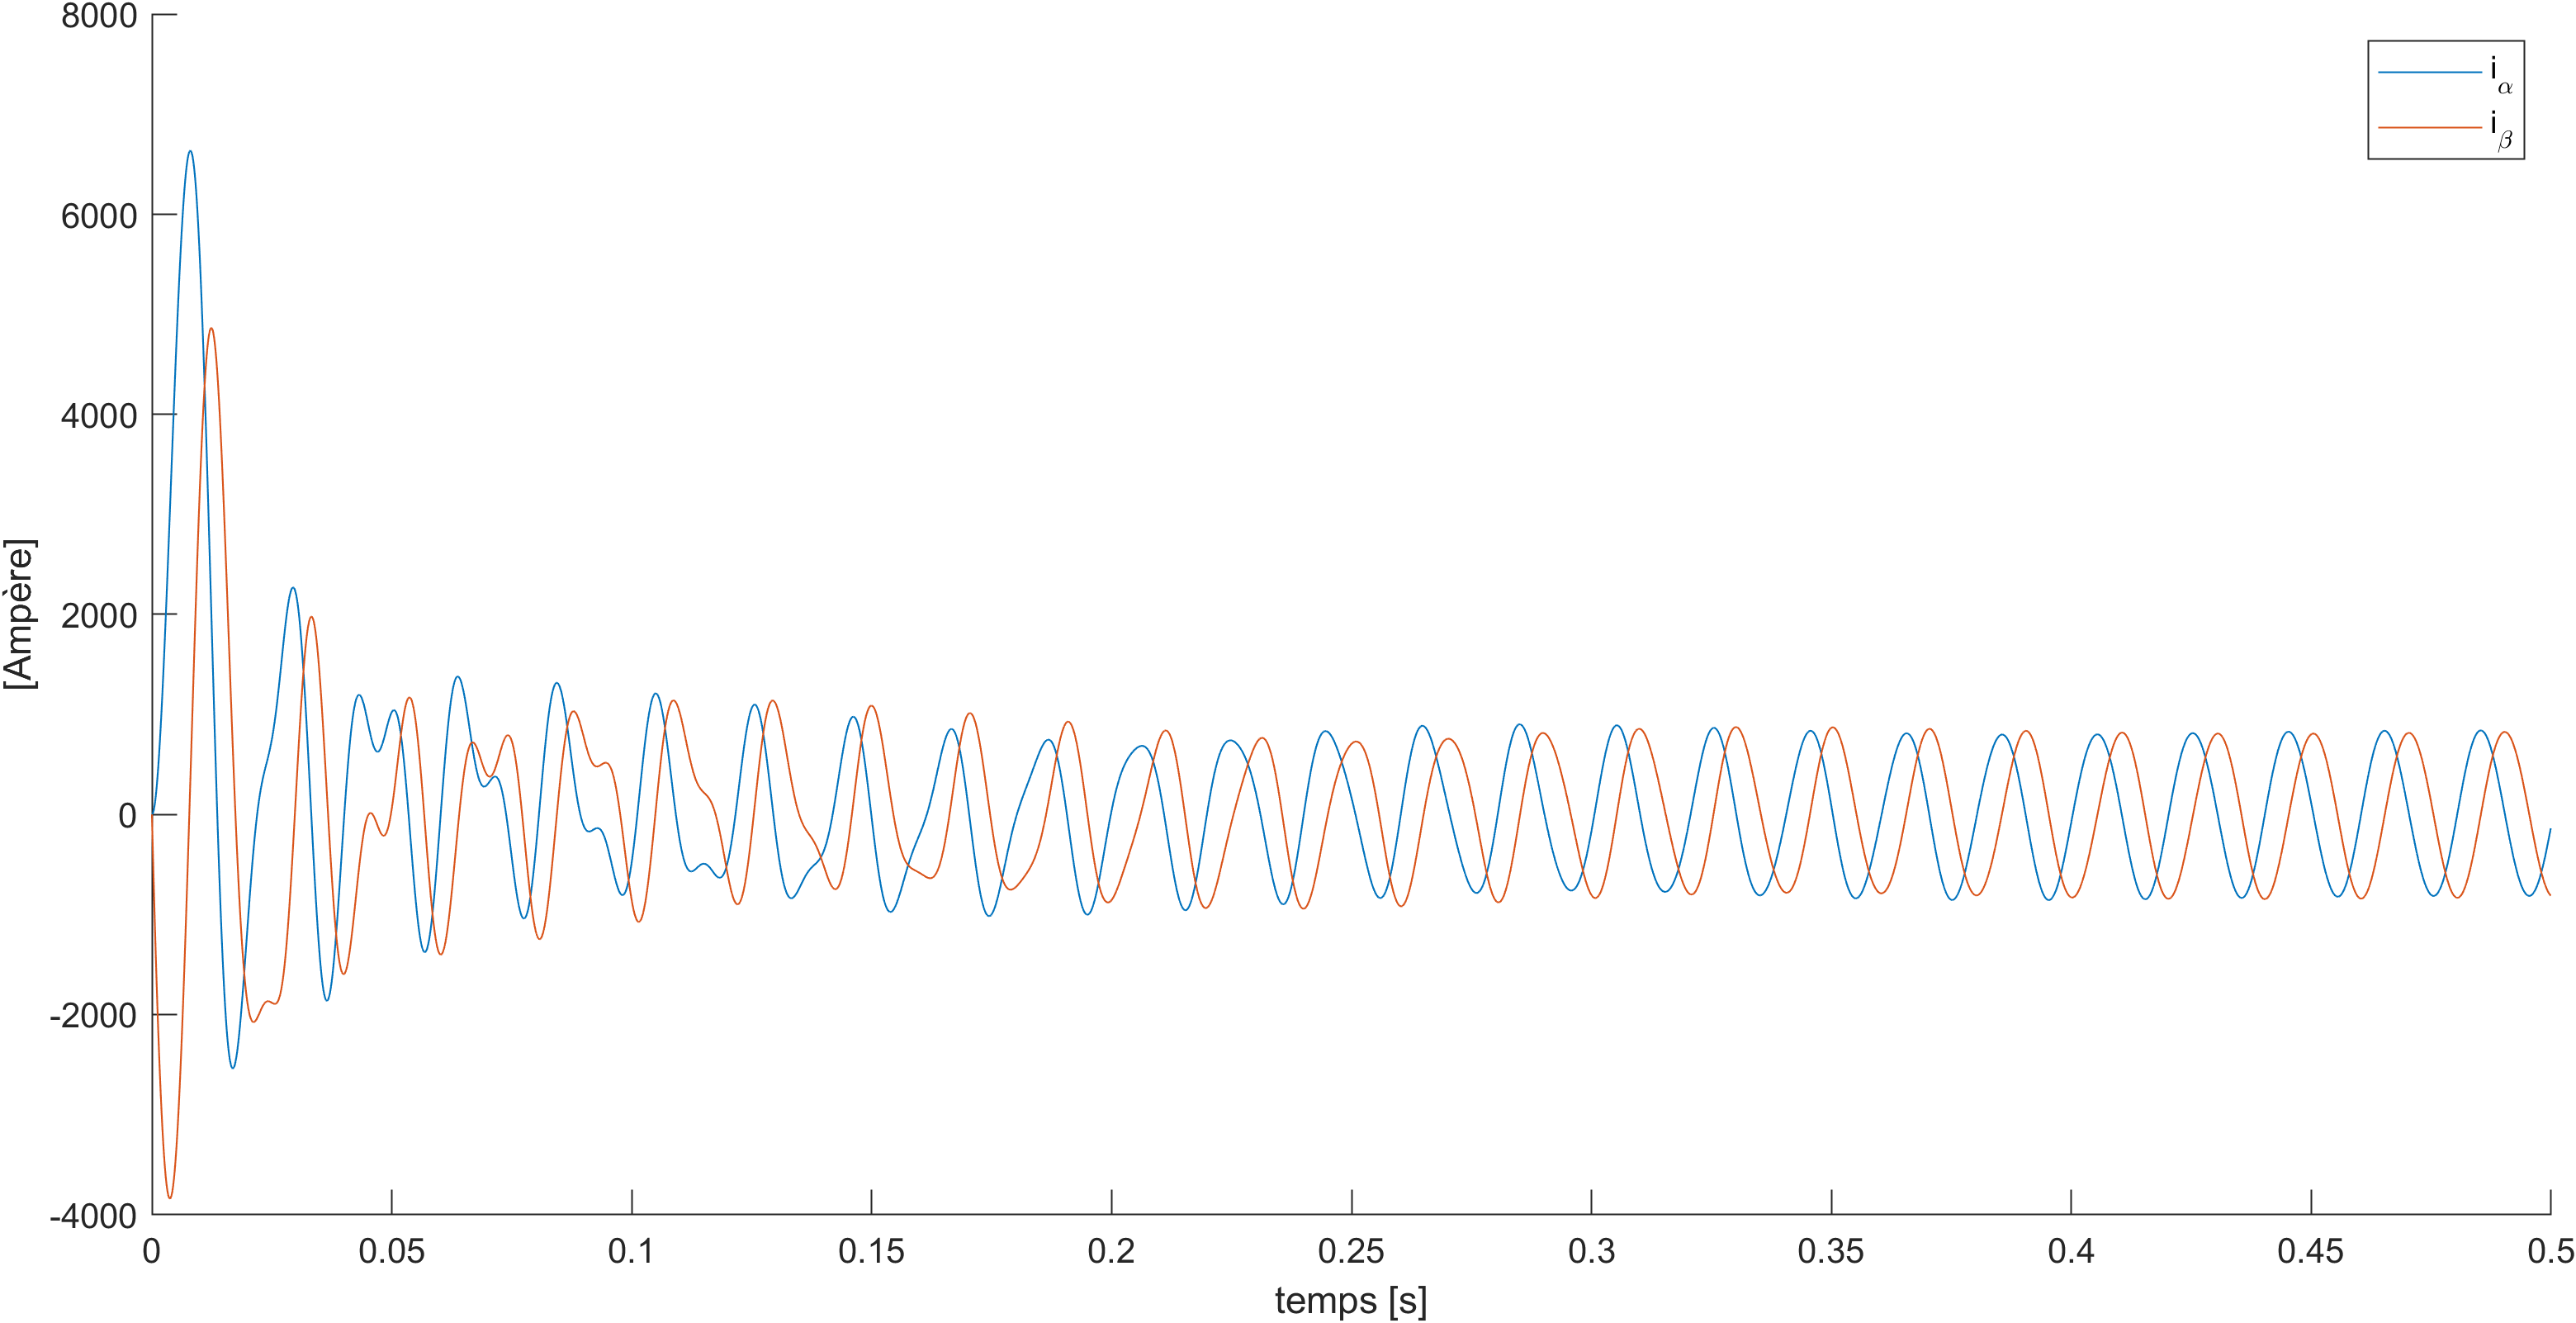
\includegraphics[width=0.8\textwidth]{simusMATLAB/MADA/ir_alphabeta.png} 
    \caption{Courants mesurées dans le repère $\alpha\beta$ de la MADA au long du temps.}
    \label{img-simuMADA-ir_alphabeta}
\end{figure}


\begin{figure}[!h]
    \centering
    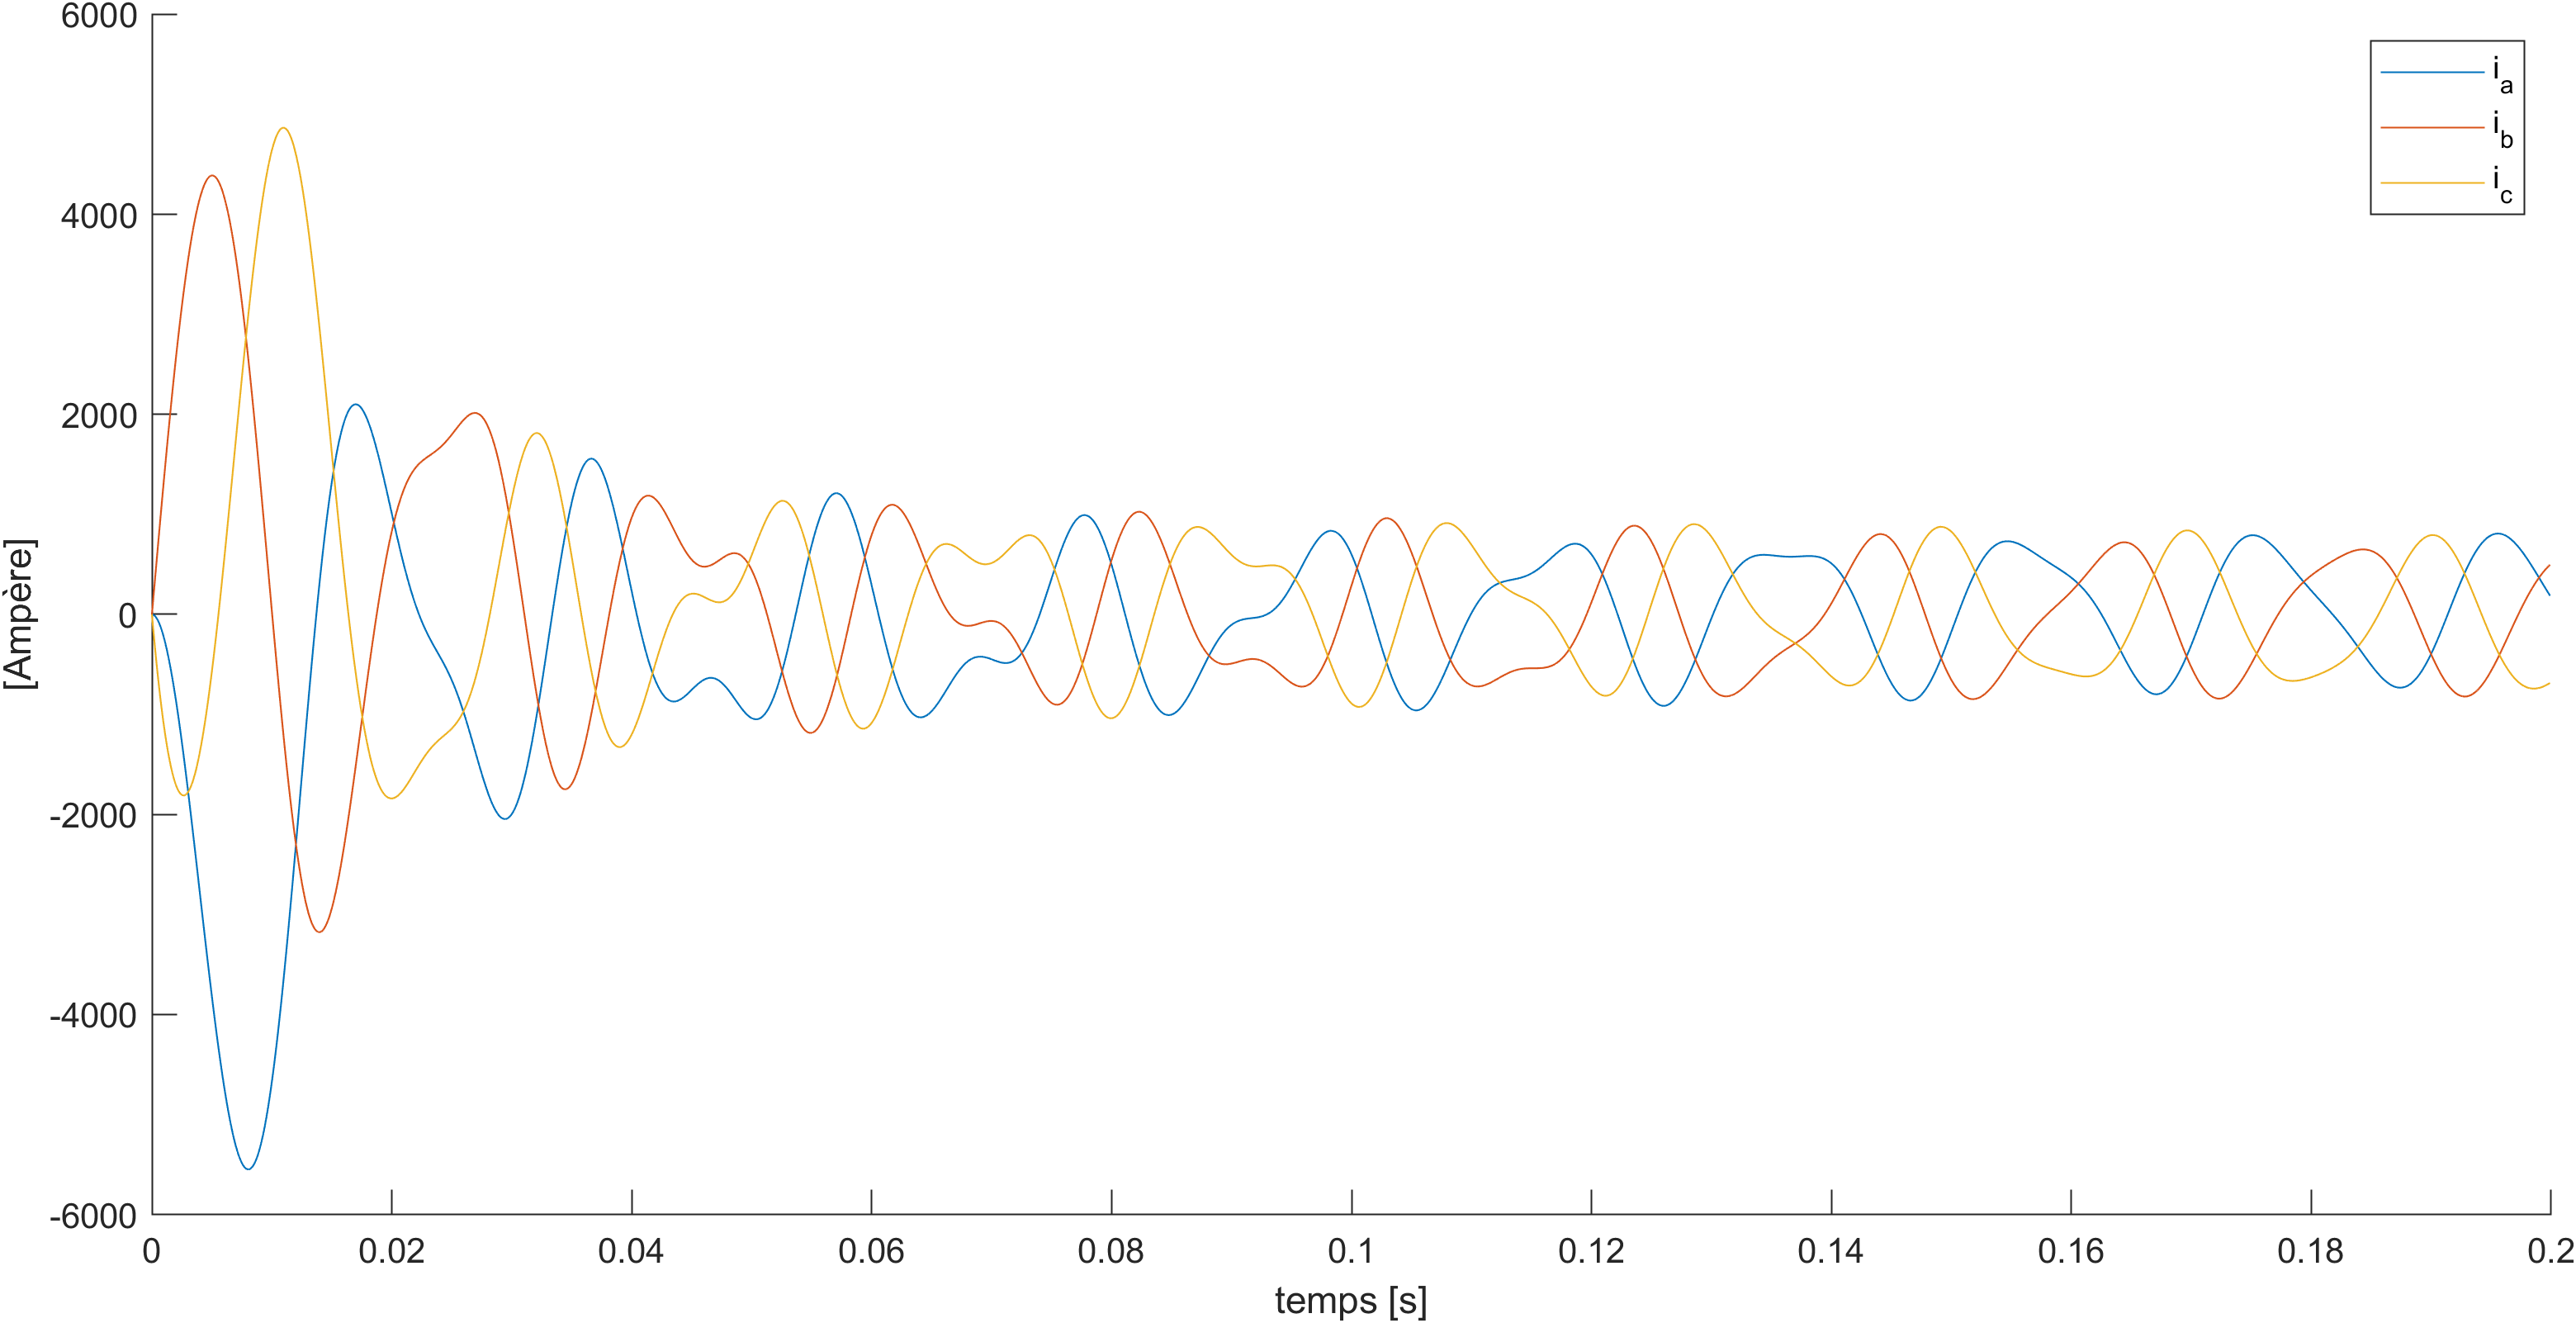
\includegraphics[width=0.8\textwidth]{simusMATLAB/MADA/is_abc.png} 
    \caption{Courants statoriques triphasées de la MADA mesurées au cous du temps.}
    \label{img-simuMADA-is_abc}
\end{figure}

En ce qui concerne les tensions mesurées pendant la simulation, les figures \ref{img-simuMADA-vs_abc} et \ref{img-simuMADA-vs_dq} montrent un comportement similaire aux simulations précédentes réalisées avec MAS, ce qui démontre l'efficacité des transformations de Park et de Concordia appliquées. La période transitoire et la stabilisation des flux à l'intérieur de la machine sont également visibles sur la Figure \ref{img-simuMADA-fluxes}.


\begin{figure}[!h]
    \centering
    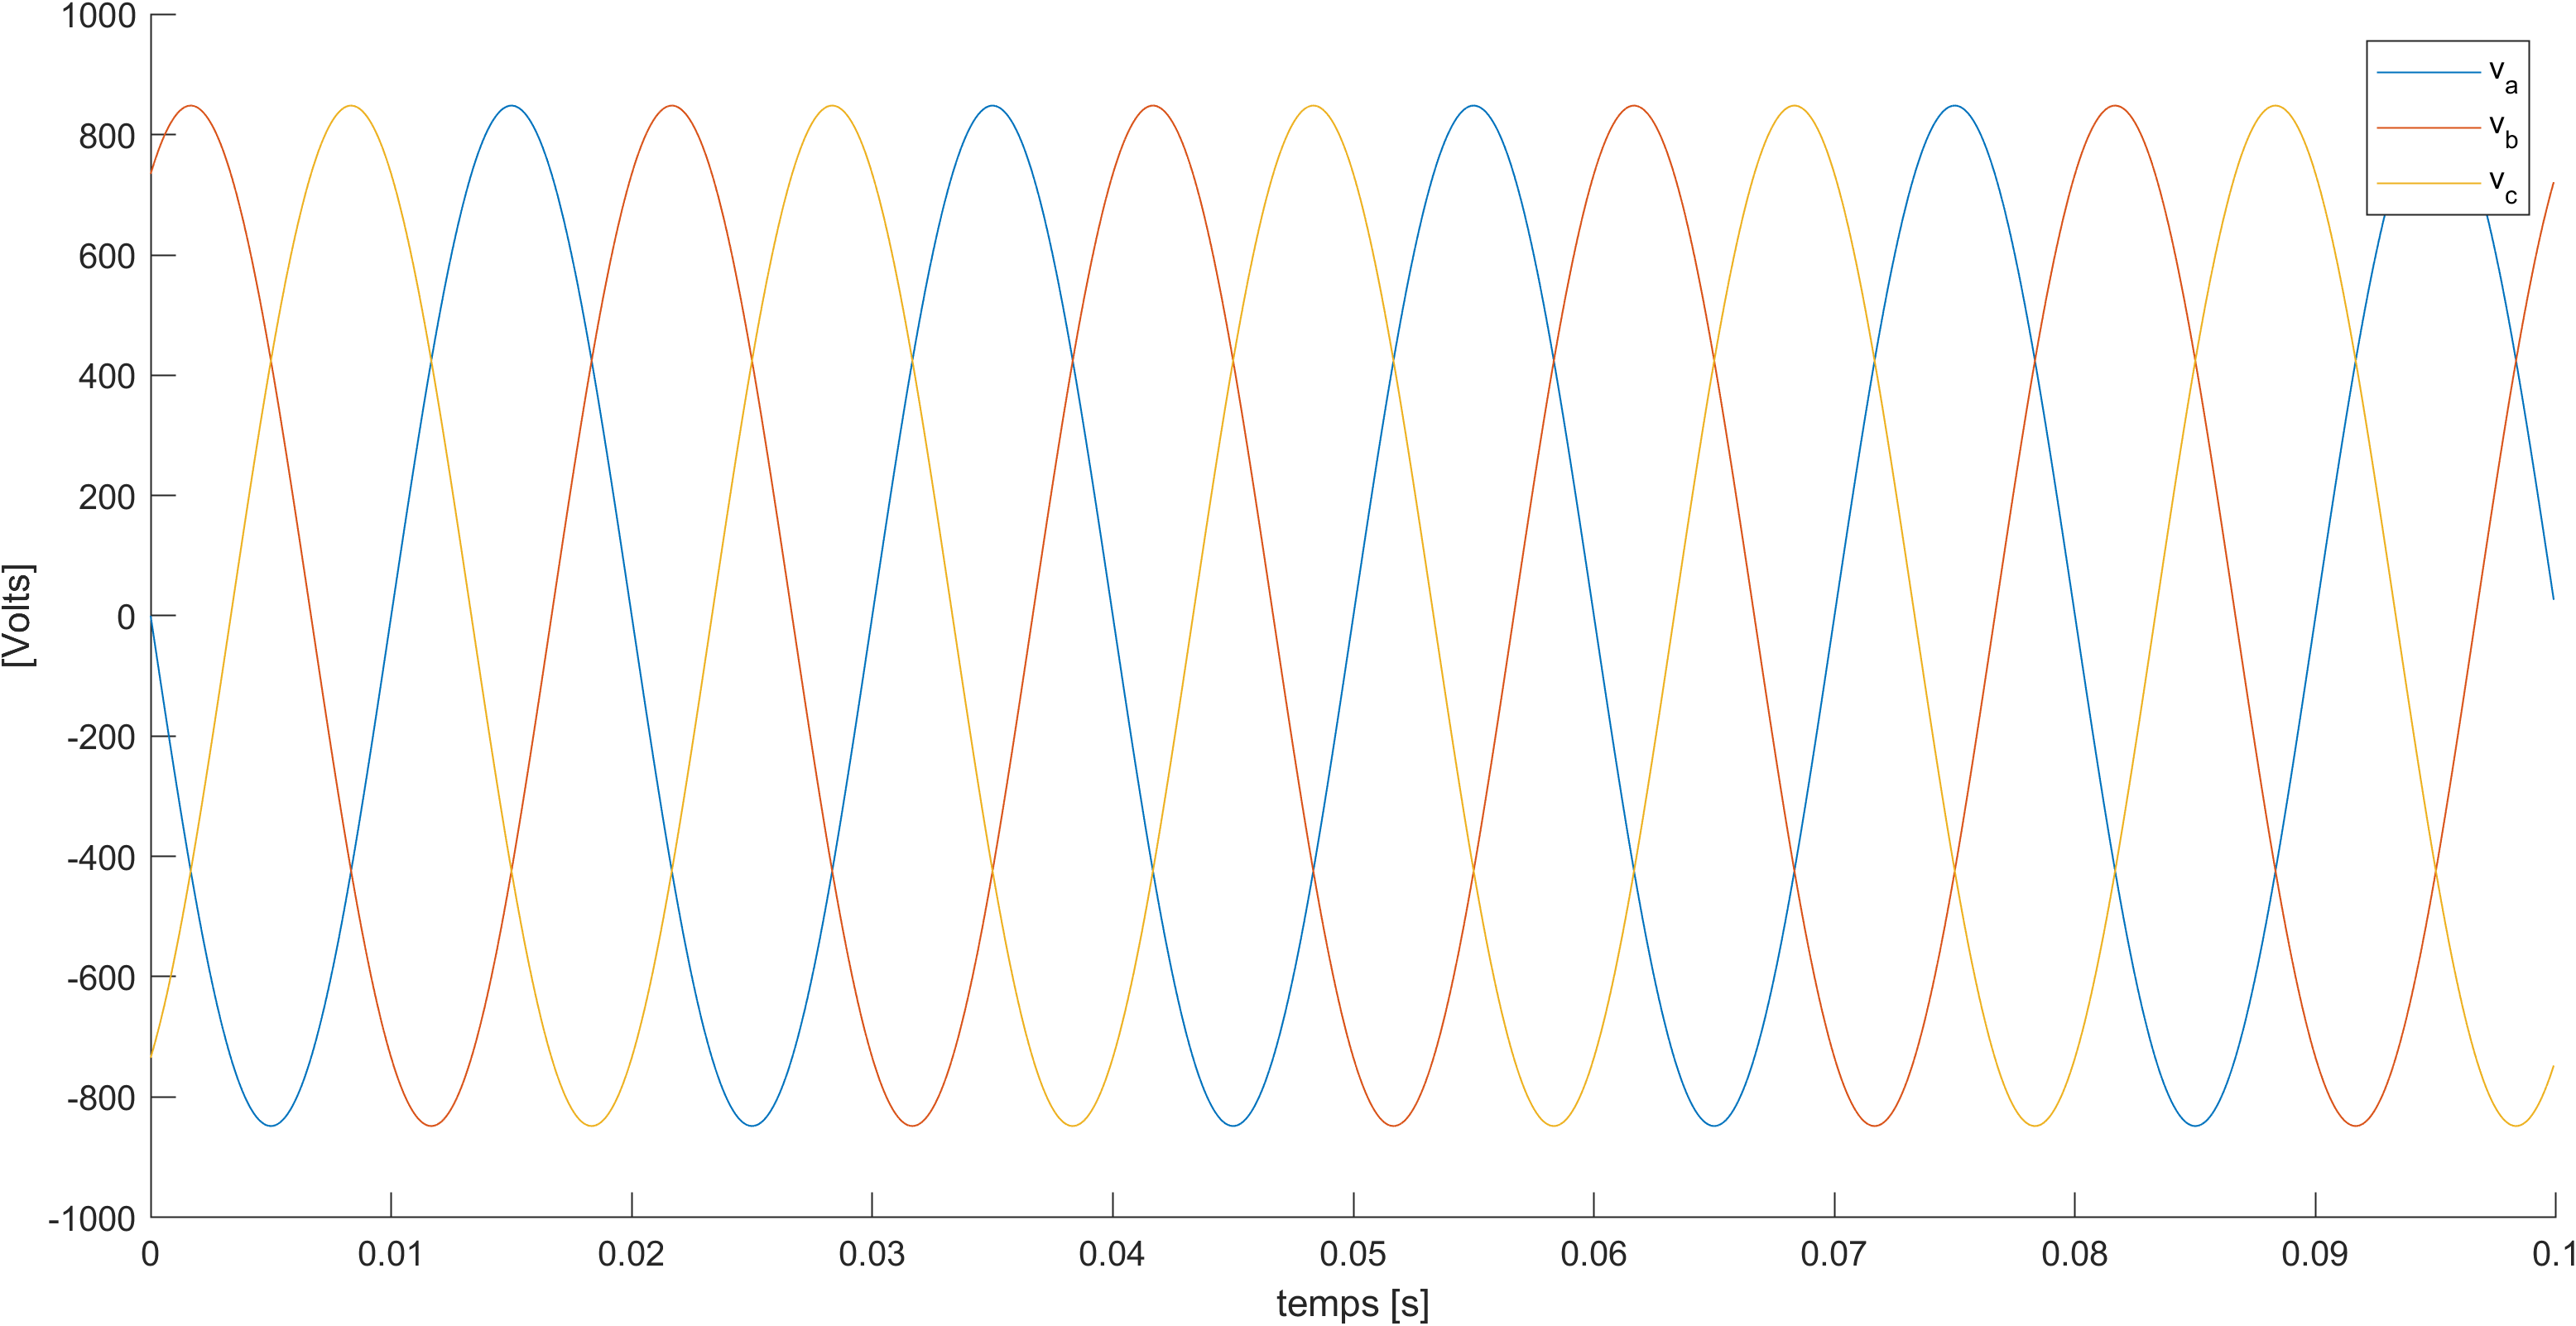
\includegraphics[width=0.8\textwidth]{simusMATLAB/MADA/vs_abc.png} 
    \caption{Tensions statoriques triphasées de la MADA mesurées au cours du temps.}
    \label{img-simuMADA-vs_abc}
\end{figure}


\begin{figure}[!h]
    \centering
    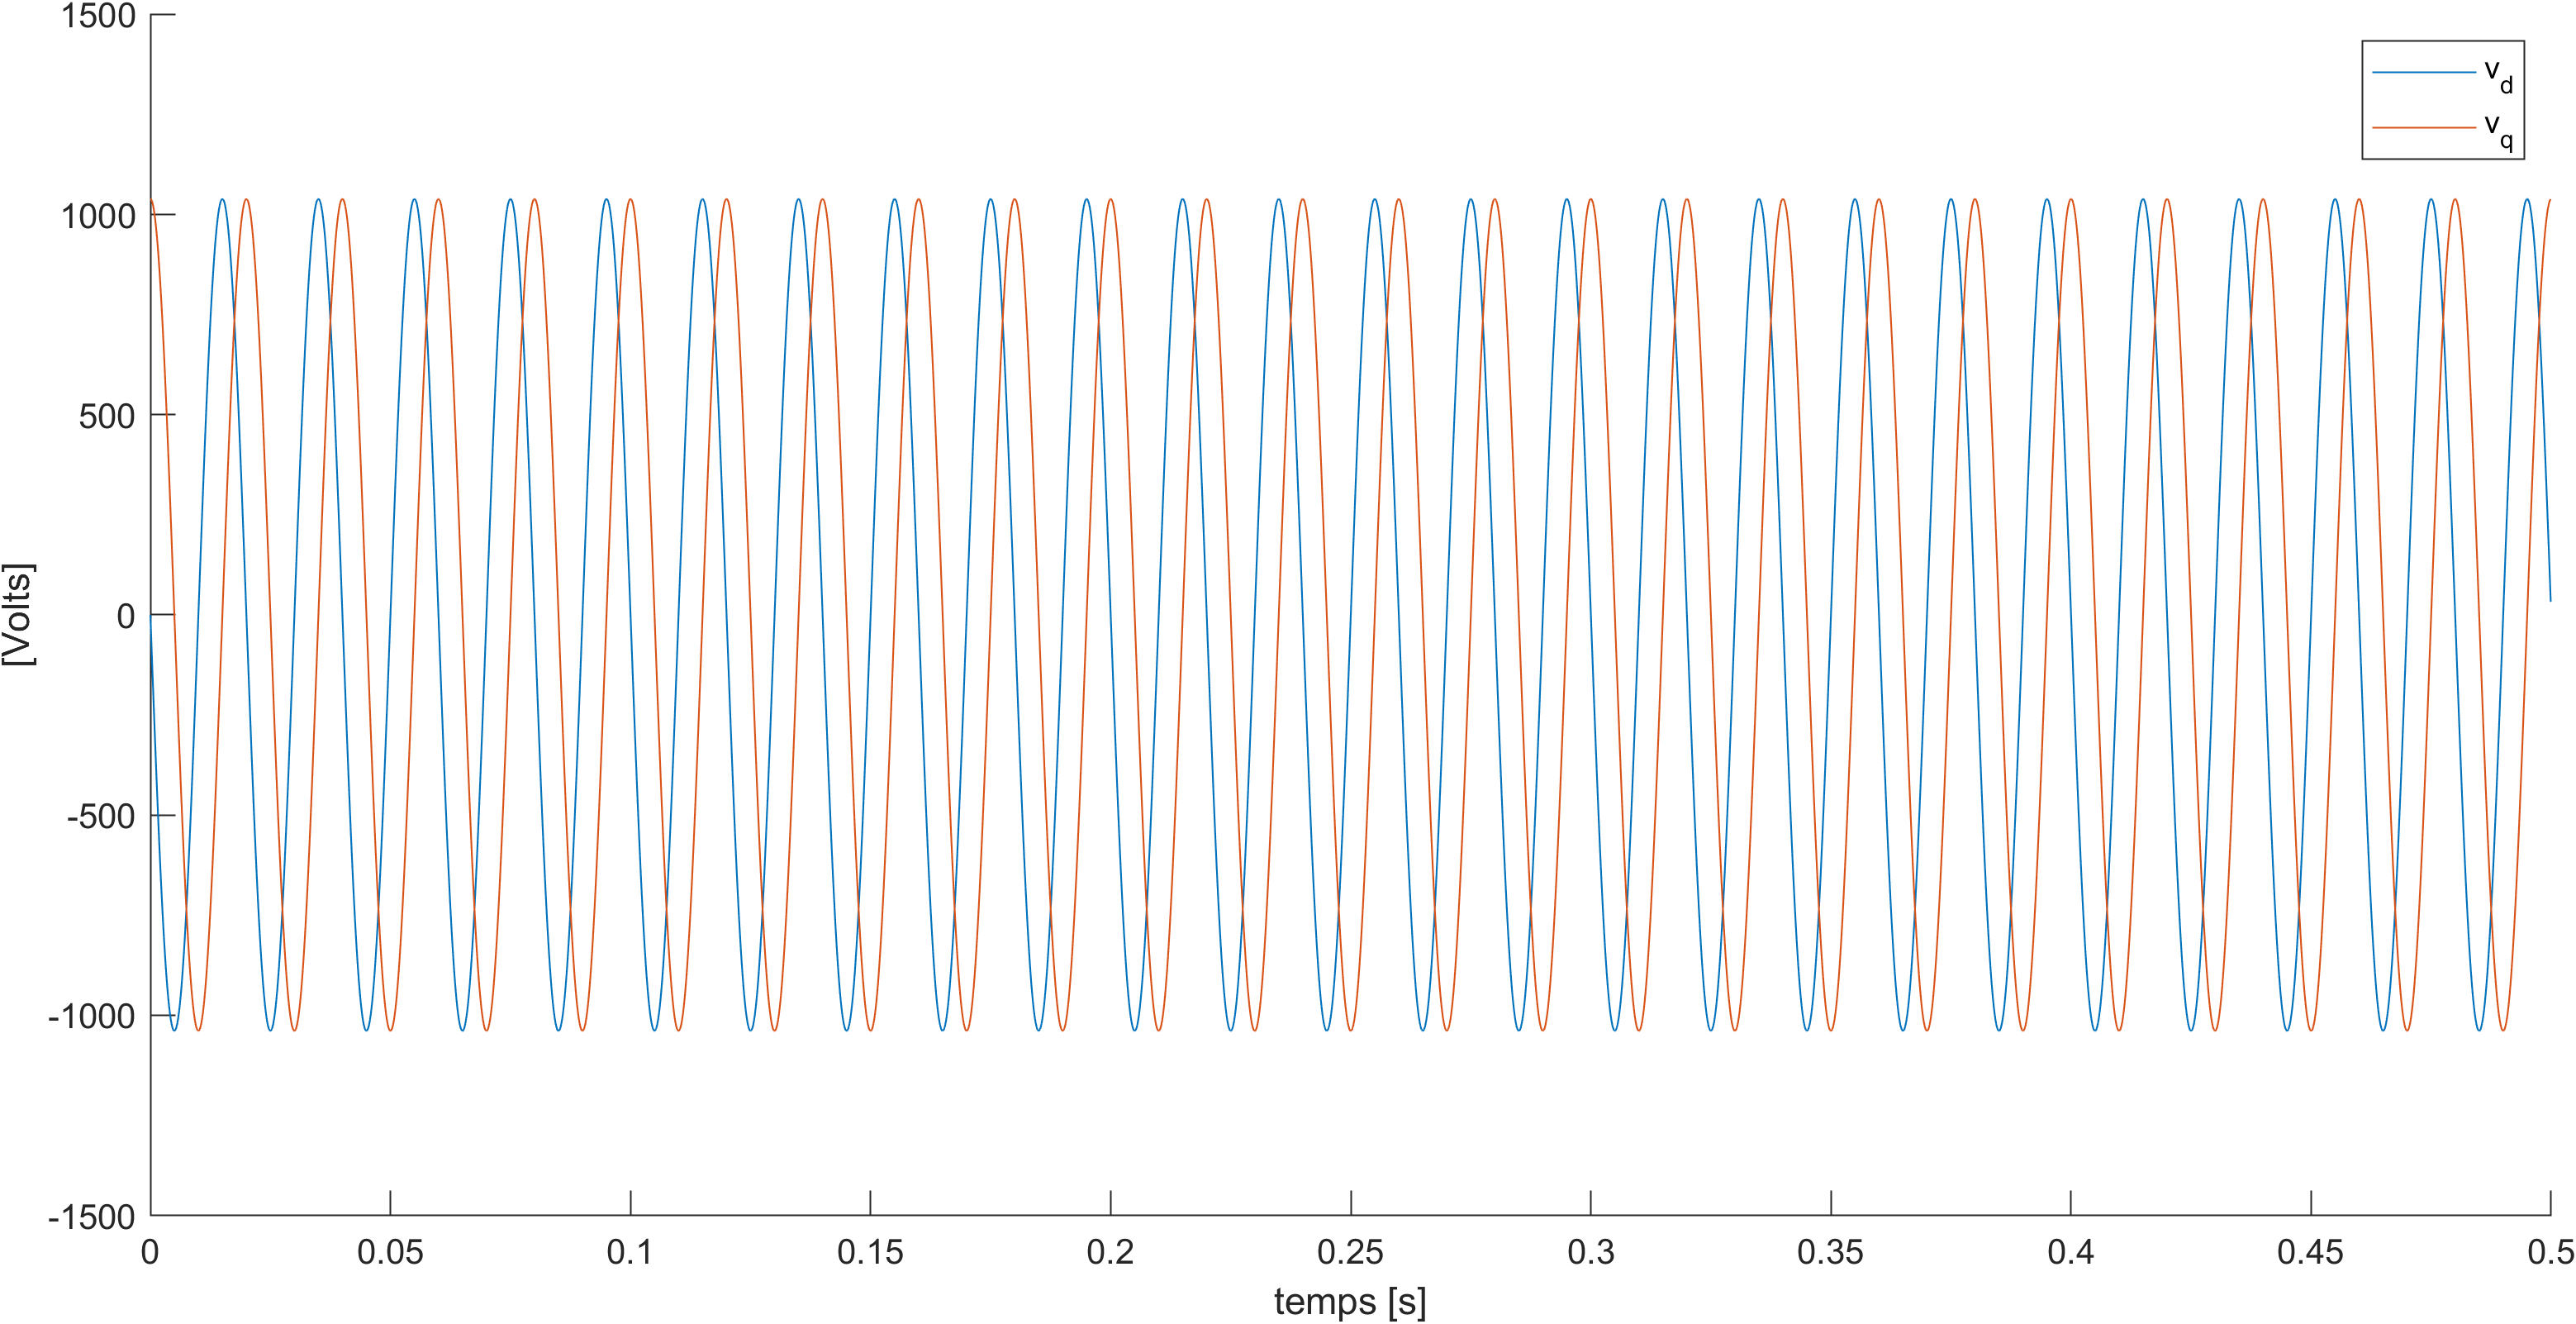
\includegraphics[width=0.8\textwidth]{simusMATLAB/MADA/vs_dq.png} 
    \caption{Tensions statoriques dq de la MADA mesurées au cours du temps.}
    \label{img-simuMADA-vs_dq}
\end{figure}


\begin{figure}[!h]
    \centering
    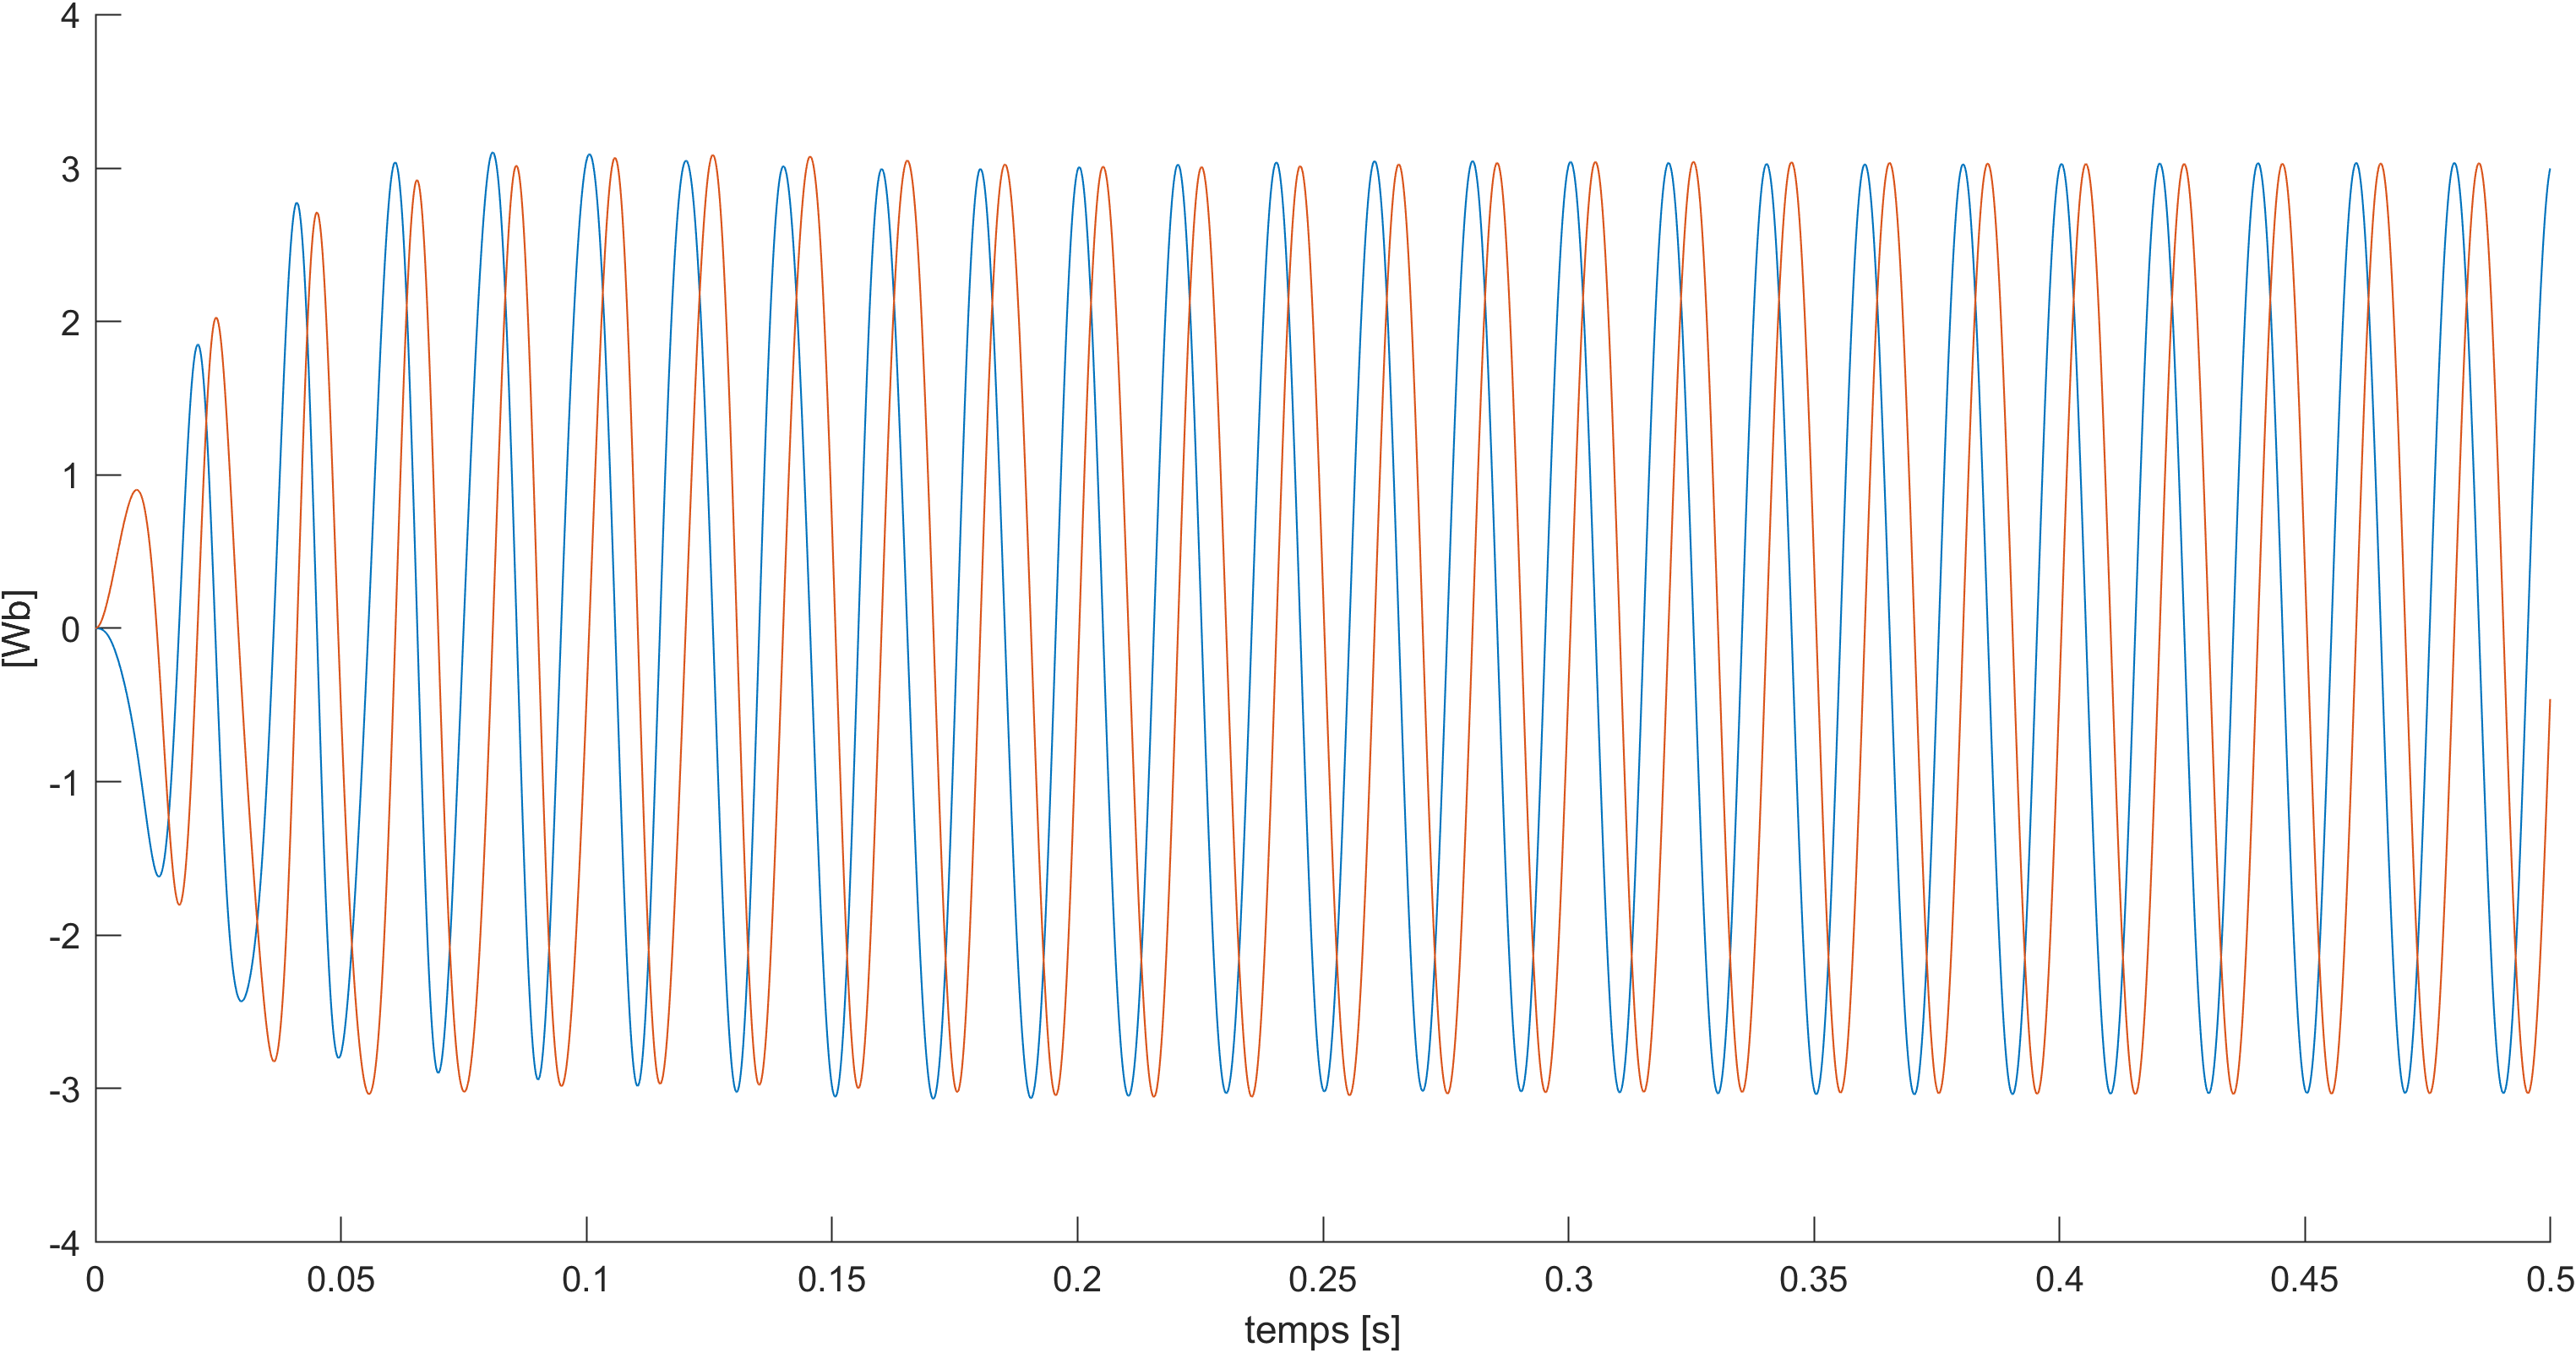
\includegraphics[width=0.8\textwidth]{simusMATLAB/MADA/fluxes.png} 
    \caption{Fluxes dq de la MADA mesurées au cours du temps.}
    \label{img-simuMADA-fluxes}
\end{figure}


En ce qui concerne le couple de la machine, sa puissance et couple, d'après les figures \ref{img-simuMADA-Ce}, \ref{img-simuMADA-P} et \ref{img-simuMADA-torque} respectivement, de fortes oscillations ont été constatées dans son régime transitoire jusqu'à ce qu'il se stabilise aux valeurs respectives de plateau.


\begin{figure}[!h]
    \centering
    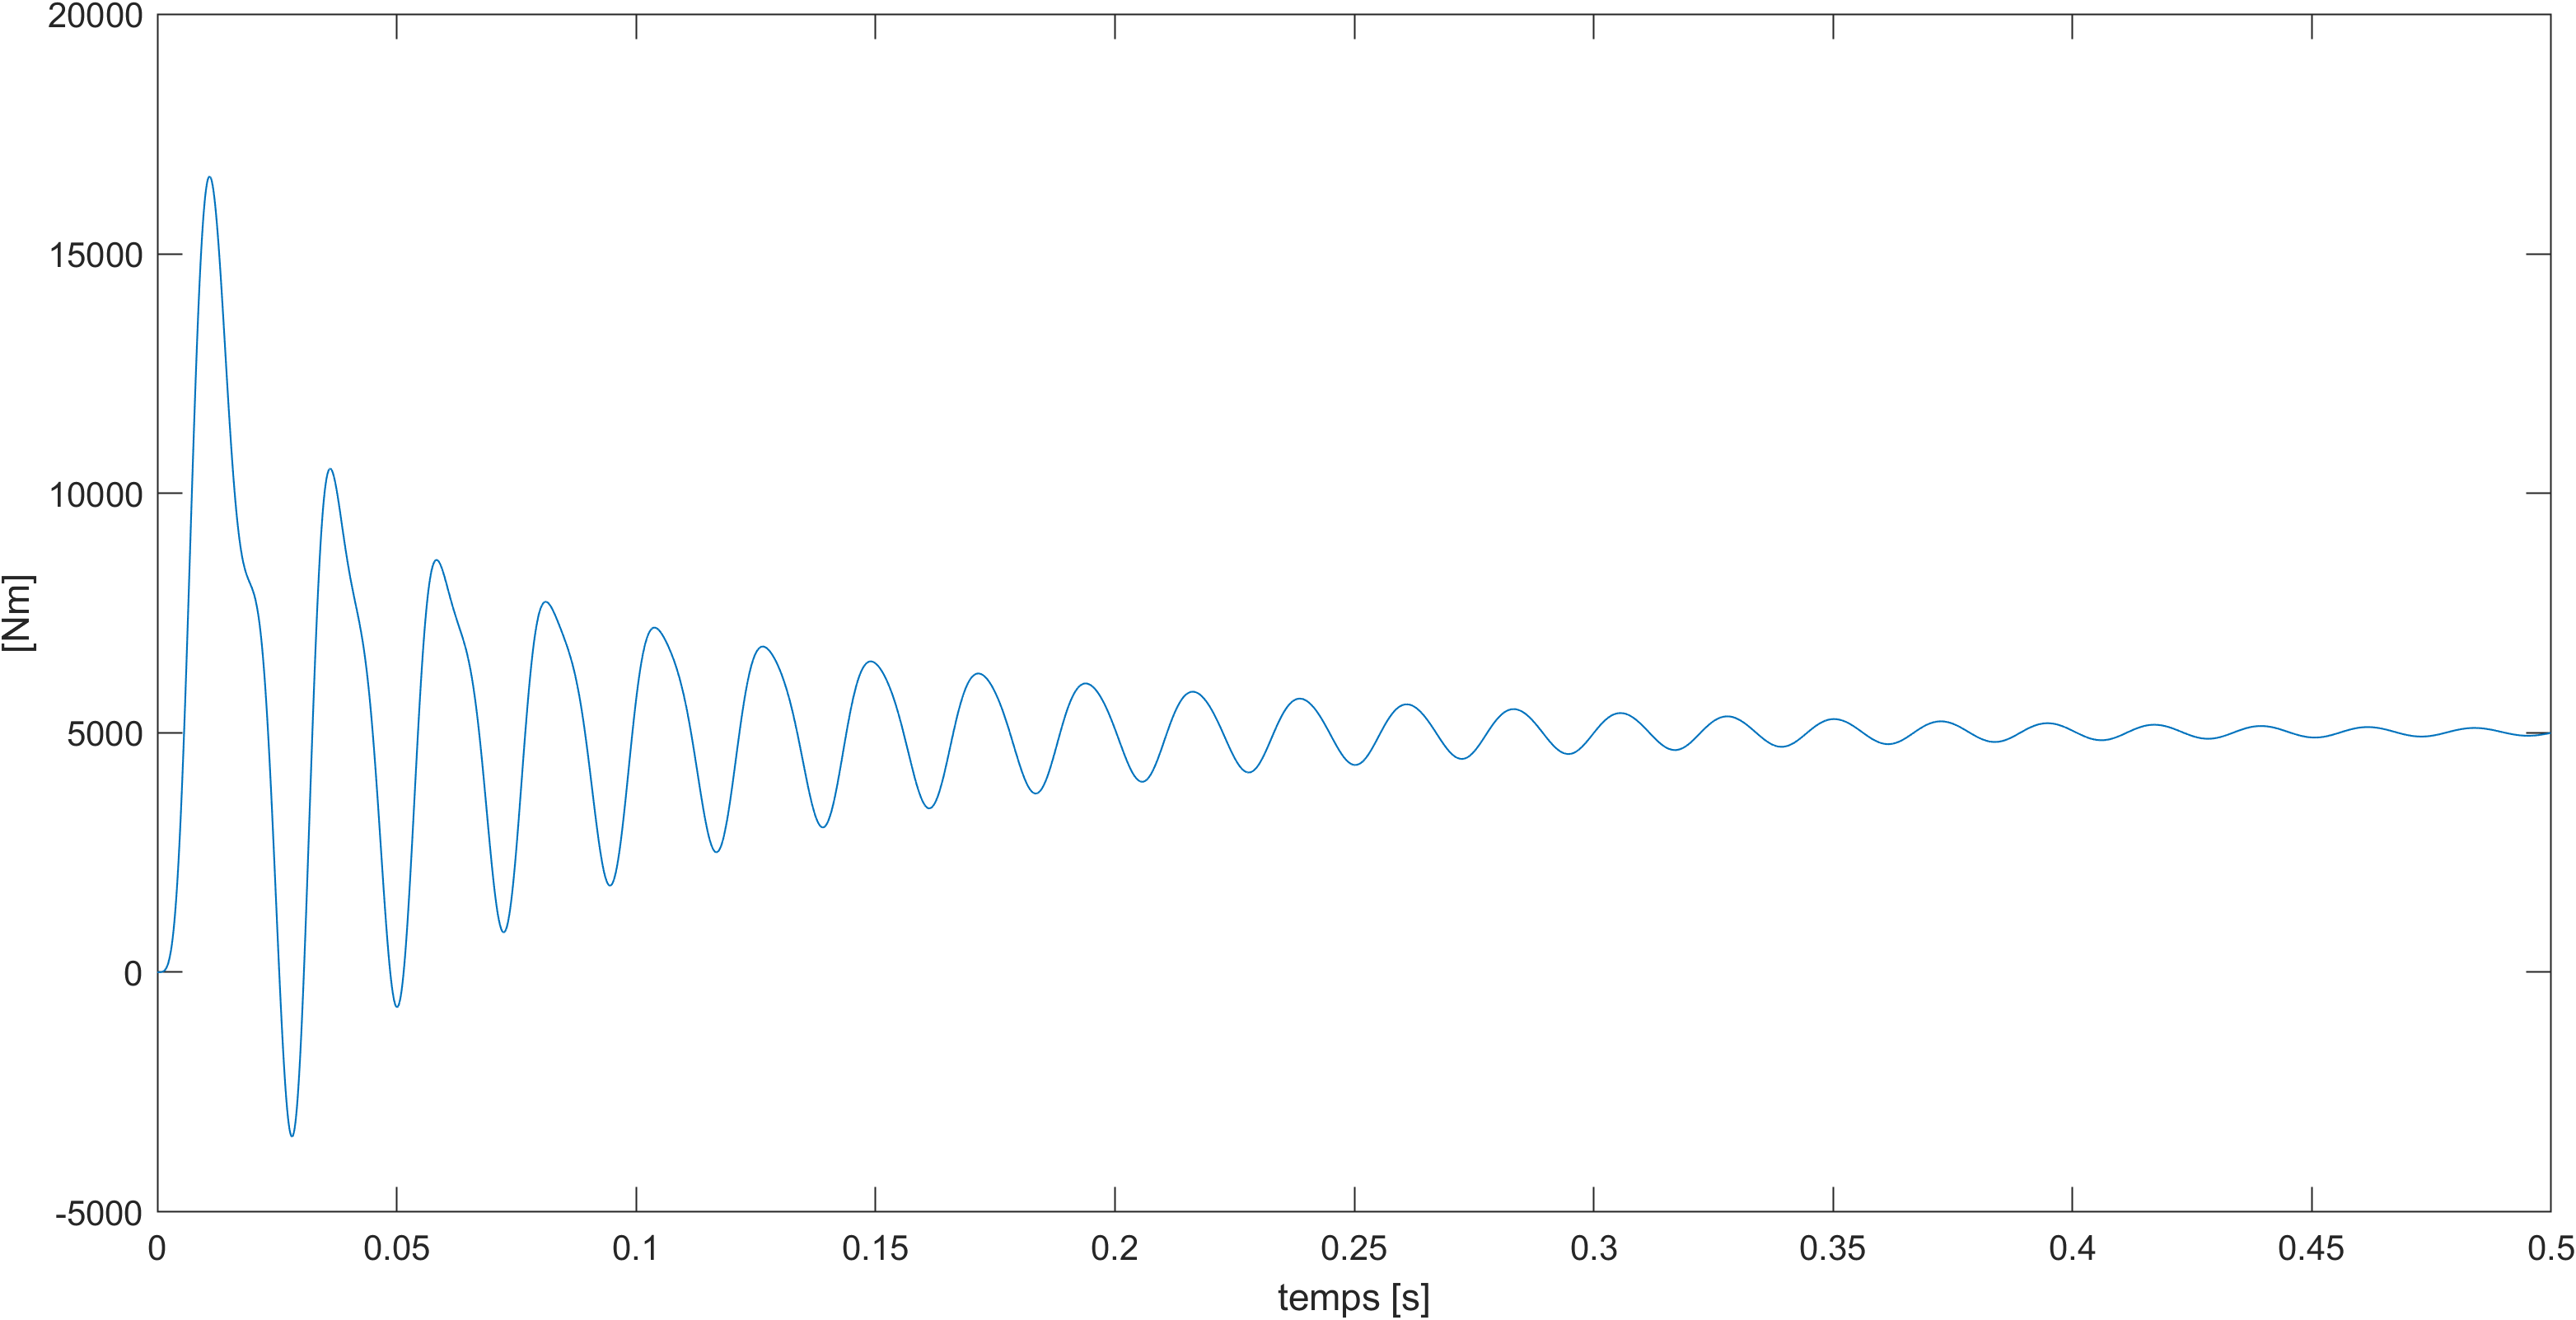
\includegraphics[width=0.8\textwidth]{simusMATLAB/MADA/Ce.png} 
    \caption{Couple de la MADA mesurée au cours du temps}
    \label{img-simuMADA-Ce}
\end{figure}


\begin{figure}[!h]
    \centering
    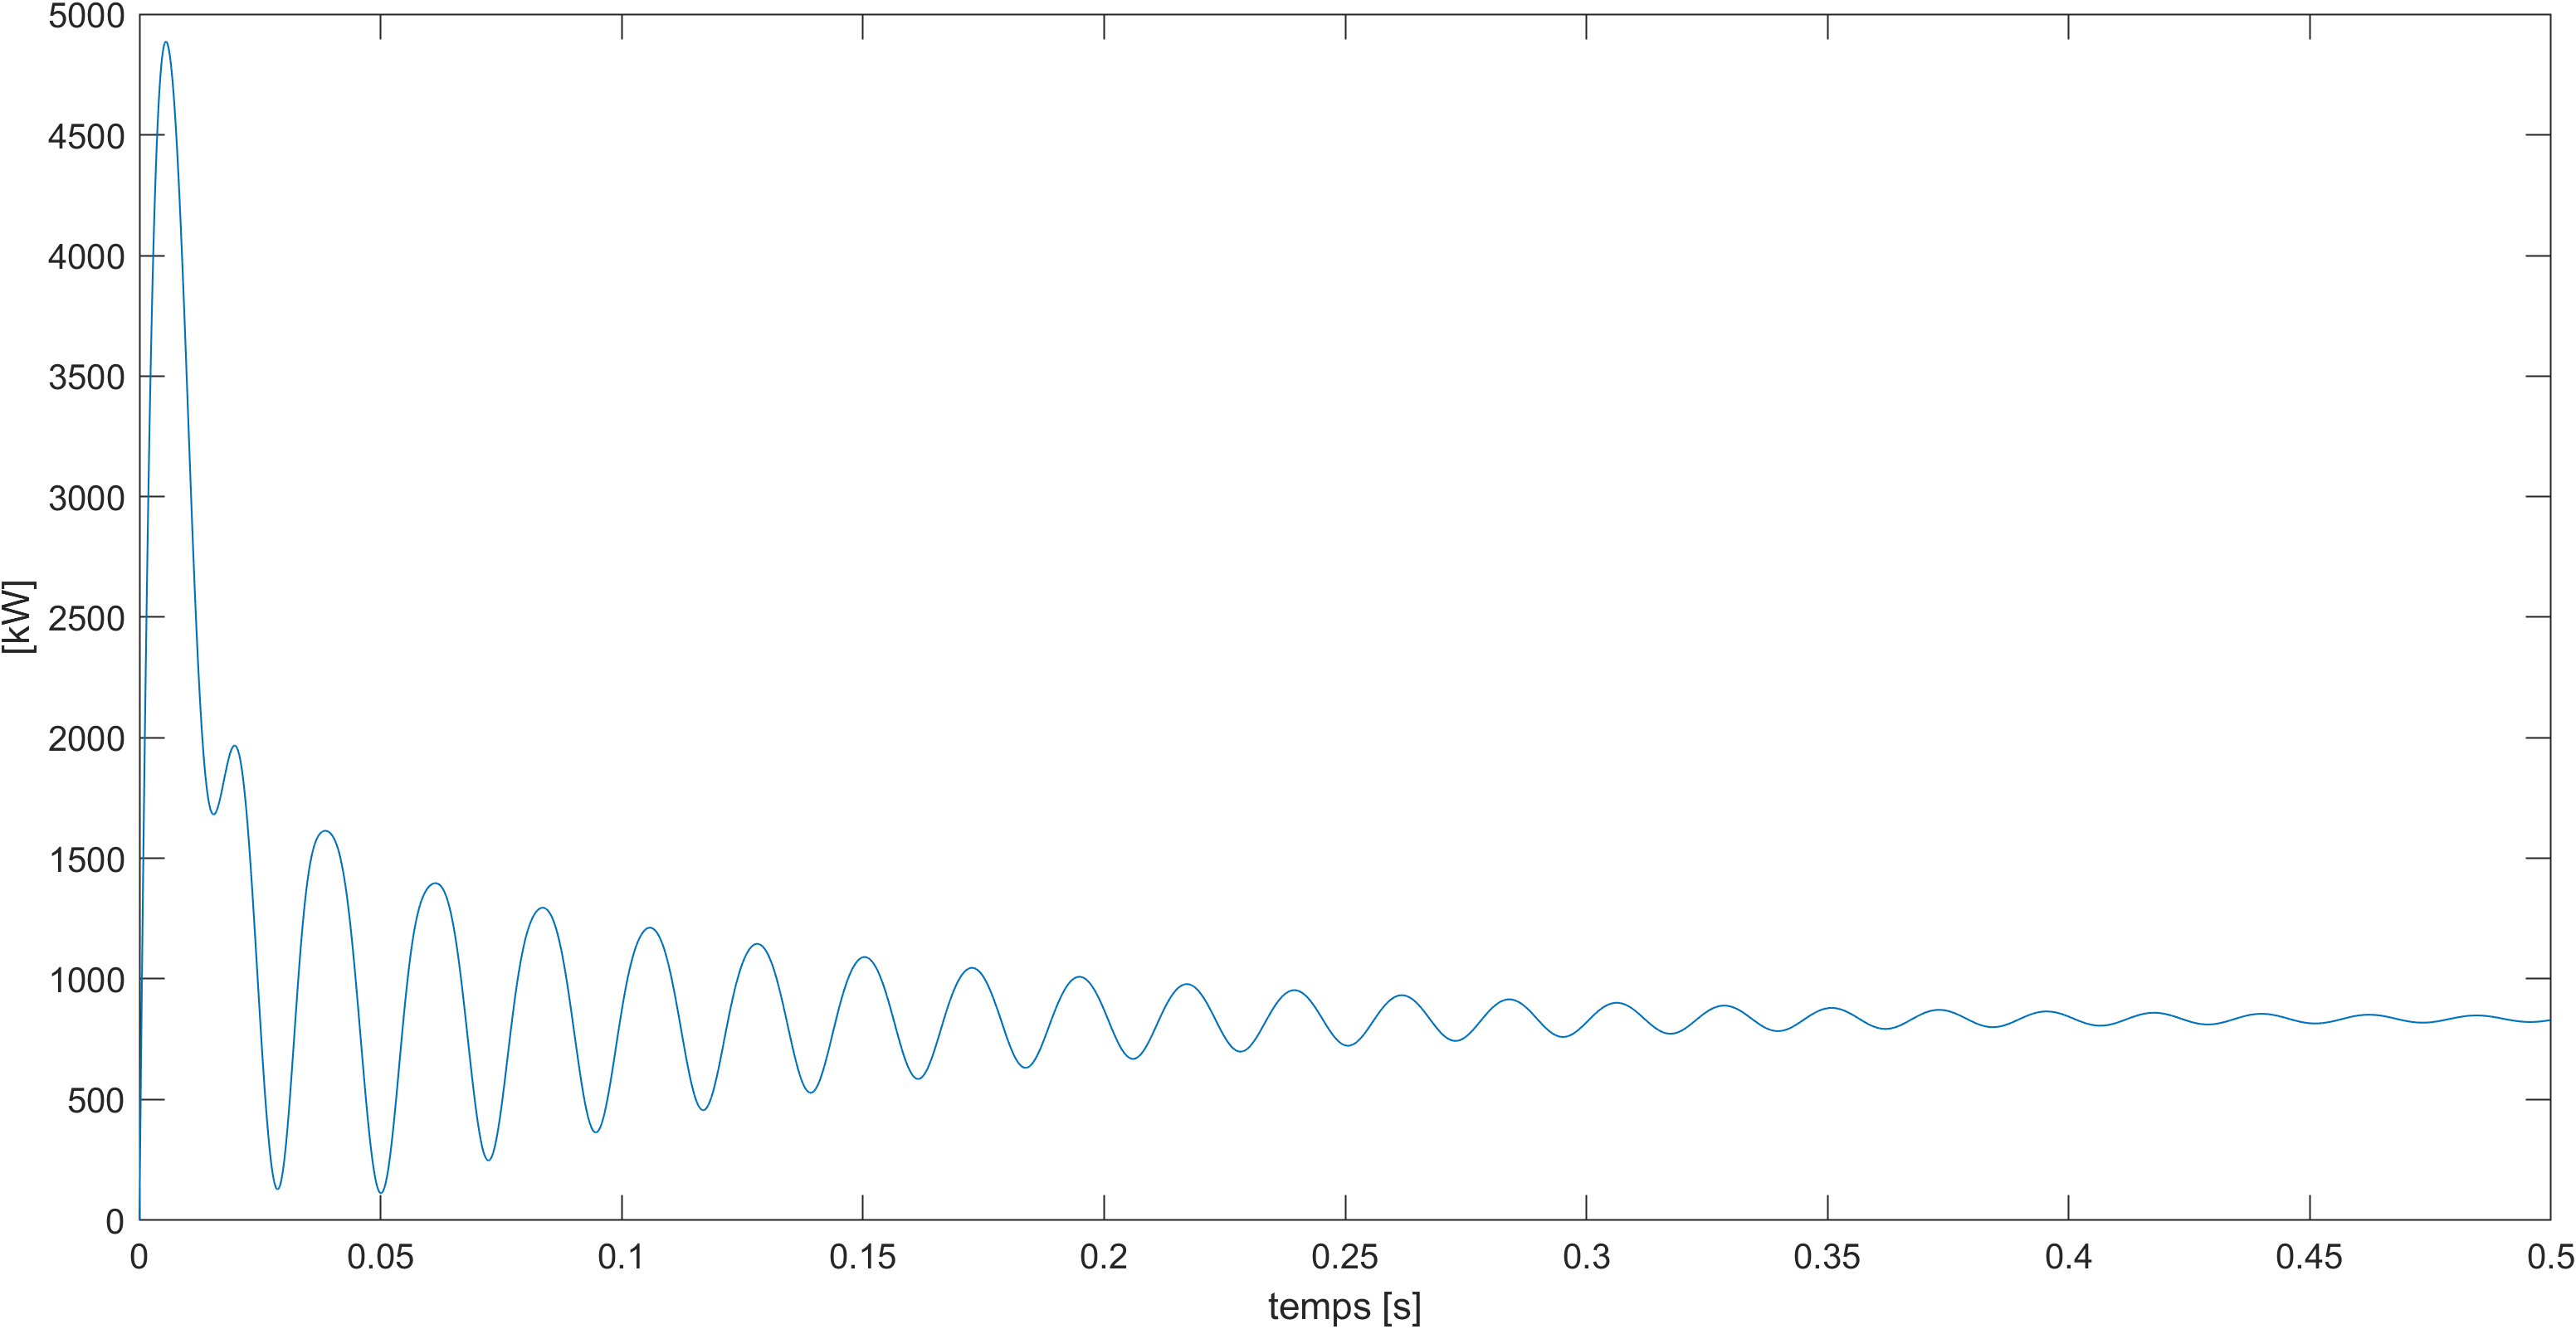
\includegraphics[width=0.8\textwidth]{simusMATLAB/MADA/P.png} 
    \caption{Courbe de la puissance de démarrage de la MADA.}
    \label{img-simuMADA-P}
\end{figure}


\begin{figure}[!h]
    \centering
    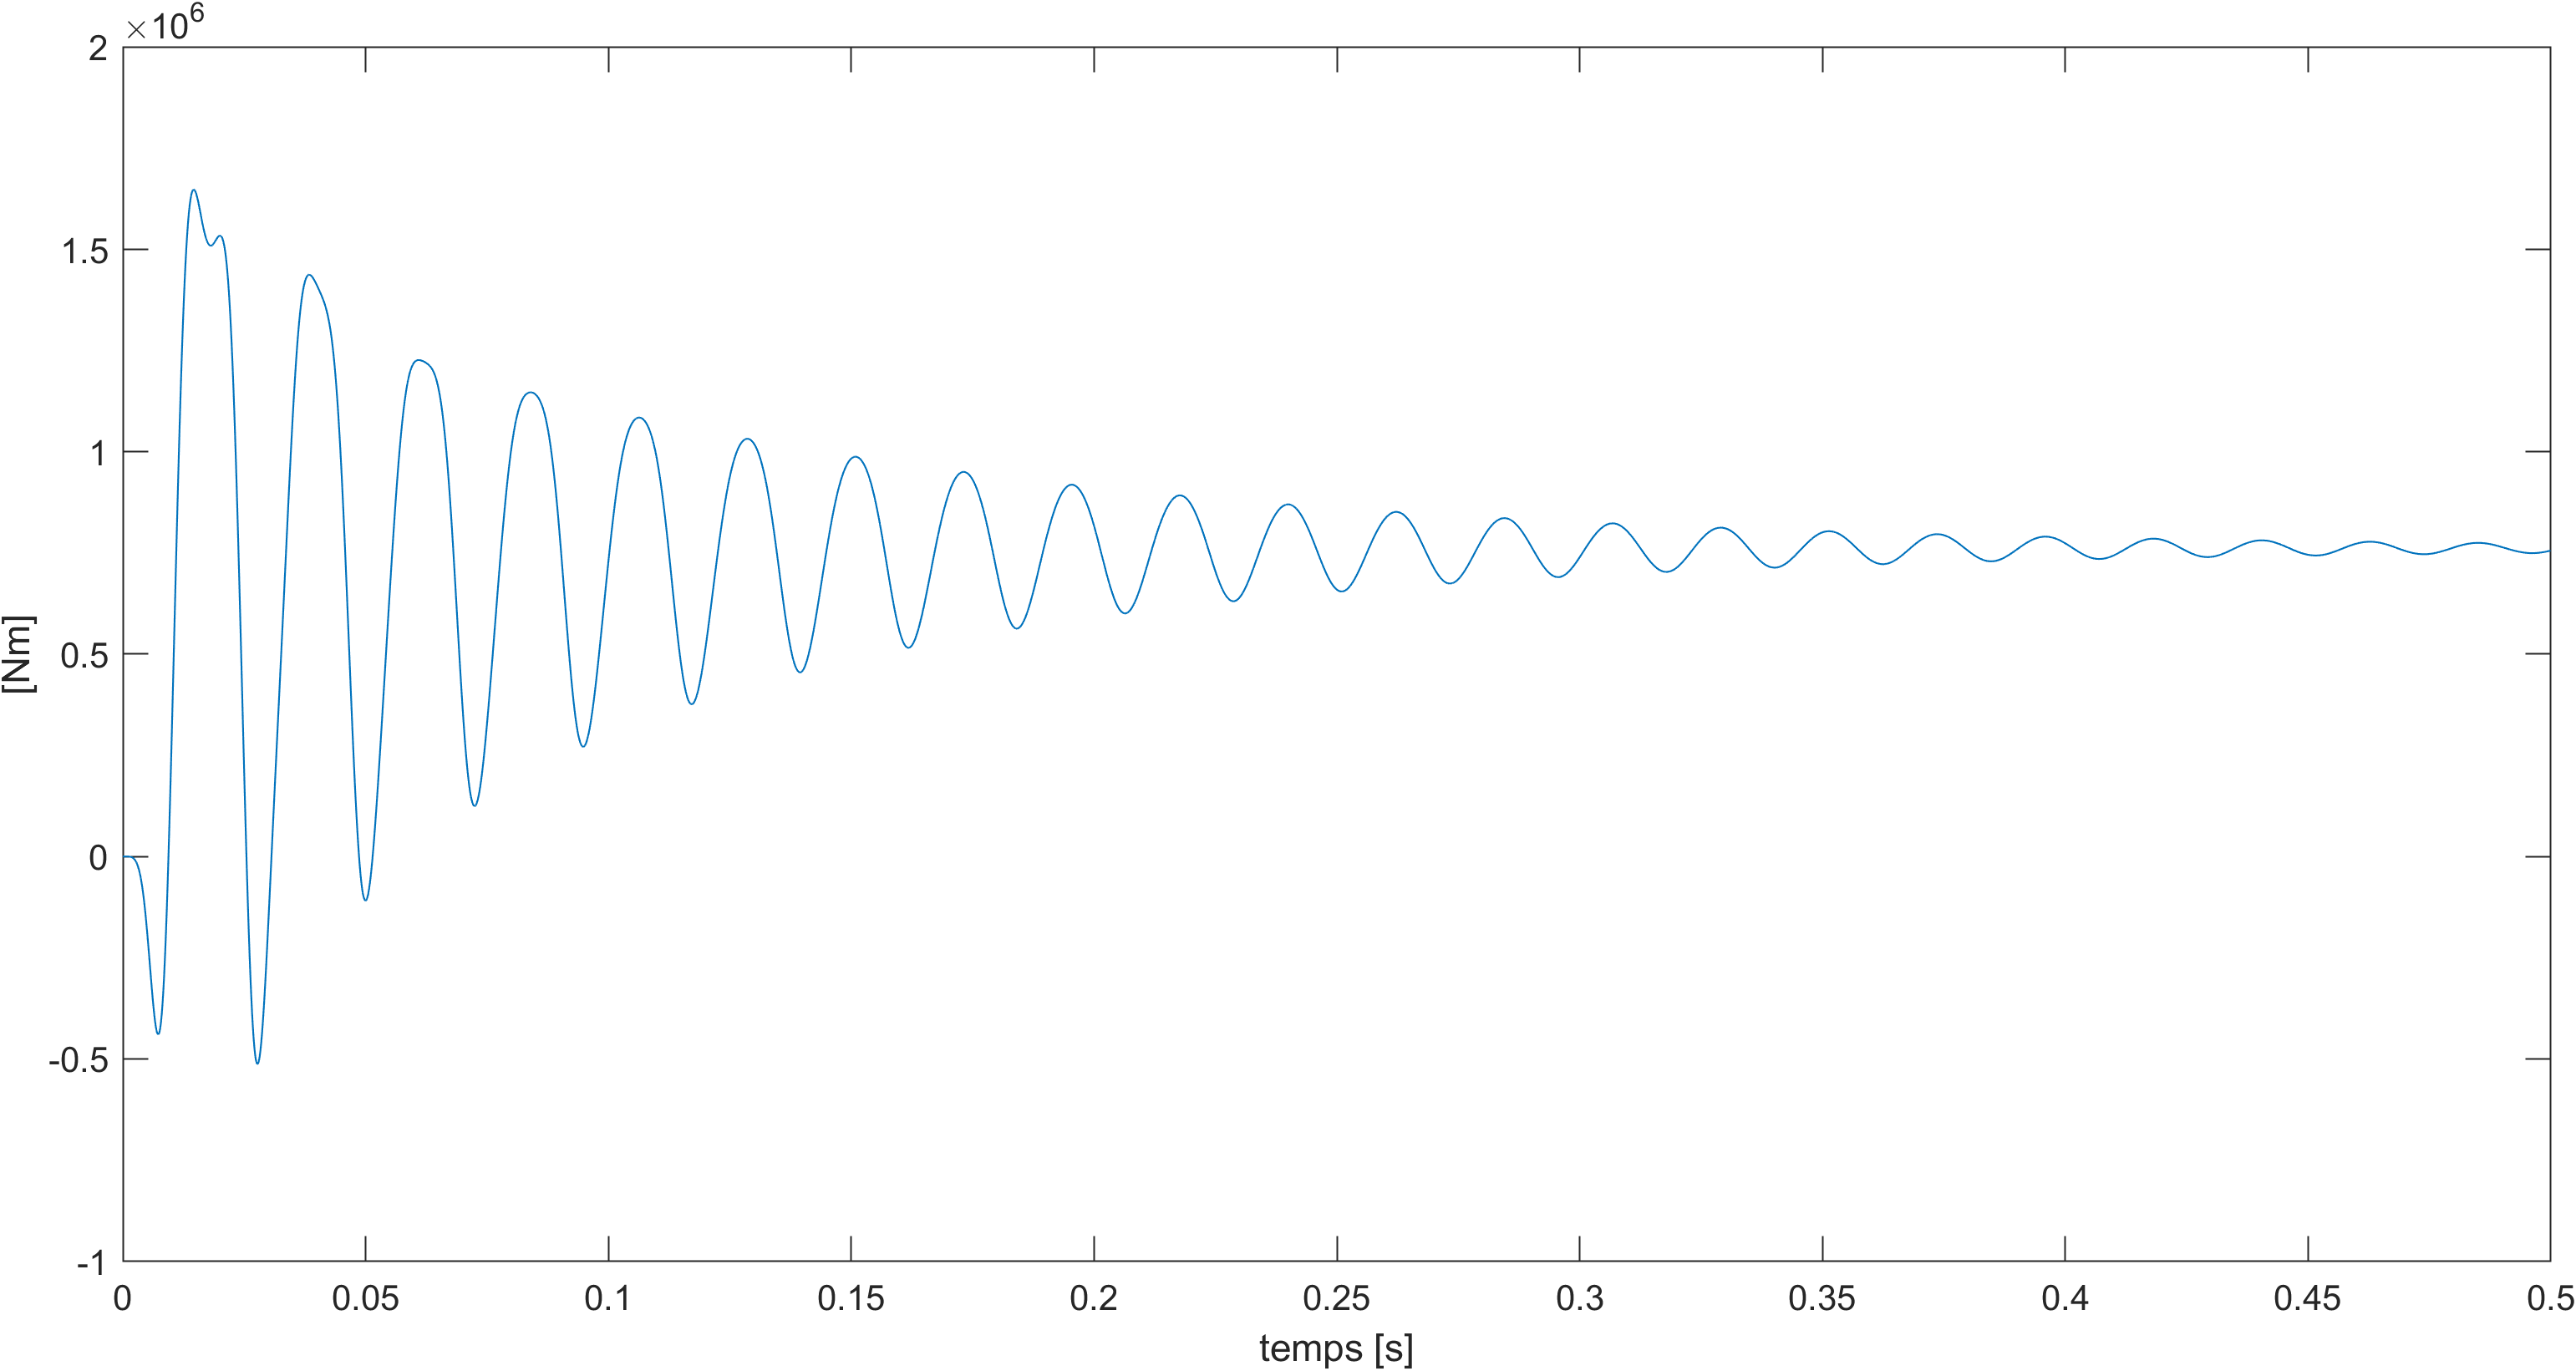
\includegraphics[width=0.8\textwidth]{simusMATLAB/MADA/torque.png} 
    \caption{Courbe du torque de démarrage de la MADA.}
    \label{img-simuMADA-torque}
\end{figure}


Après avoir simulé la MADA comme une machine à induction, plusieurs essais ont été effectués avec les contrôleurs de l'architecture présentée dans les figures \ref{img-diagMADA} et \ref{img-MADA}, mais sans résultats positifs. Pour le contrôleur, les coefficients $K_p$ et $\tau_i$ ont été calculés en utilisant la relation \ref{eq:MADA7} présentée. Ainsi, $K_p = 26,3158$ et $\tau_i = 0,0139$ ont été initialement calculés à l'aide de \ref{eq:MADA7} comme suit :


\begin{equation*}
    \left\{
    \begin{aligned}
        K_p =& \frac{1}{\alpha \cdot R_eq} \\
        \tau_i =& \beta \cdot \frac{L_eq}{R_eq}
    \end{aligned}
    \right. \;; \;\;
    \left\{
    \begin{aligned}
        L_{eq} =& L_r - \frac{M^2}{L_s} \\
        R_{eq} =& R_r
    \end{aligned}
    \right.
\end{equation*}

Simulink a présenté des erreurs de boucle algébrique dans plusieurs tentatives de simulation. Afin d'essayer de corriger l'erreur, le pas fixe du solveur Range-Kutta d'ordre 4 a été réduit, puis d'autres modèles de solveur disponibles dans Simulink ont été testés, ainsi que des modifications des paramètres de la machine et même des modifications de l'architecture du contrôleur, qui se sont toutes révélées infructueuses. En outre, pour tenter de corriger les erreurs de simulation, les contrôleurs autorégulateurs PI de Simulink ont été testés, mais ils n'ont pas non plus réussi à calculer les coefficients, affichant un message indiquant que le calcul divergeait et demandant de réduire le pas de simulation ou de changer de modèle. 

Parmi les architectures de contrôleurs autres que celles présentées ci-dessus qui ont été testées figurent les architectures présentées par BOYETTE \cite{Boyette2006}, illustrées dans les figures \ref{img-arc1}, \ref{img-arc2} et \ref{img-arc3}. Malheureusement, les erreurs du logiciel Simulink ont persisté et il n'a pas été possible d'extraire des données des simulations avec les contrôleurs de puissance MADA en fonctionnement.


\begin{figure}[!h]
    \centering
    \includegraphics[width=0.8\textwidth]{diagrammes/arc1.png} 
    \caption{Schéma bloc de la commande indirecte \cite{Boyette2006}}
    \label{img-arc1}
\end{figure}

\begin{figure}[!h]
    \centering
    \includegraphics[width=0.8\textwidth]{diagrammes/arc2.png} 
    \caption{Schéma bloc de la commande indirecte avec boucles de puissance \cite{Boyette2006}.}
    \label{img-arc2}
\end{figure}

\begin{figure}[!h]
    \centering
    \includegraphics[width=0.8\textwidth]{diagrammes/arc3.png} 
    \caption{Schéma bloc de la commande directe \cite{Boyette2006}.}
    \label{img-arc3}
\end{figure}


\text{ }

\FloatBarrier
\newpage
\section{Conclusions}

Cette étude s'est concentrée sur la simulation et l'analyse des machines asynchrones à cage et à double alimentation (MADA), explorant les méthodes de contrôle et leur application dans des systèmes de conversion d'énergie. L'usage de MATLAB/Simulink a permis d'examiner les performances des techniques de contrôle vectoriel pour réguler efficacement la vitesse des machines asynchrones à cage et la gestion de la puissance pour les MADA.

L'application des transformations de coordonnées, telles que Park, Clarke, et Concordia, a facilité la modélisation des dynamiques électriques et mécaniques des machines, permettant une analyse plus claire des stratégies de contrôle. Ces outils de modélisation ont été essentiels pour ajuster les paramètres de contrôle et pour identifier des voies d'amélioration des performances des machines étudiées.

Les simulations ont mis en évidence l'utilité des environnements logiciels pour tester divers paramètres et configurations, offrant un moyen économique et flexible d'évaluer les performances sans les contraintes des tests physiques. Cette approche a été bénéfique pour l'optimisation des systèmes de contrôle et la validation des concepts théoriques.

Néanmoins, les simulations ont également révélé certaines limitations, comme les difficultés liées à la résolution de boucles algébriques et les défis de convergence des solveurs. Ces problématiques ont souligné l'importance d'une modélisation et d'une sélection de paramètres attentives pour garantir des résultats fiables et représentatifs.

En somme, l'étude a apporté des contributions significatives à la compréhension des machines asynchrones à cage et à double alimentation, tout en reconnaissant la nécessité de poursuivre la recherche pour affiner les techniques de contrôle et exploiter pleinement les avantages des simulations numériques dans le développement de systèmes énergétiques avancés.

\newpage
\section{Bibliographie}
\label{sec:ref}
% Temporarily disable section titles right before the bibliography
\titleformat{\section}[block]{\Large\bfseries}{}{0pt}{\vspace{-\baselineskip}\phantom}
\bibliographystyle{unsrt}
\bibliography{references}
% Re-enable section titles after the bibliography
\titleformat{\section}[block]{\Large\bfseries}{\thesection}{1em}{}

%\newpage
%\section{Appendices}
%\input{tex_files/9_appendices.tex}

\end{document}
